% ----------------------------------------------------------------------
%                   LATEX TEMPLATE FOR PhD THESIS
% ----------------------------------------------------------------------

% based on Harish Bhanderi's PhD/MPhil template, then Uni Cambridge
% http://www-h.eng.cam.ac.uk/help/tpl/textprocessing/ThesisStyle/
% corrected and extended in 2007 by Jakob Suckale, then MPI-CBG PhD programme
% and made available through OpenWetWare.org - the free biology wiki


%: Style file for Latex
% Most style definitions are in the external file PhDthesisPSnPDF.
% In this template package, it can be found in ./Latex/Classes/
\documentclass[twoside,11pt]{PhDthesisPSnPDF}

\usepackage[utf8]{inputenc}
\usepackage[T1]{fontenc}
\usepackage{lmodern}
%\usepackage[english,french]{babel} % already in PhDthesisPSnPDF
%switching can be done with \selectlanguage{english} \selectlanguage{french}

%: Macro file for Latex
% Macros help you summarise frequently repeated Latex commands.
% Here, they are placed in an external file /Latex/Macros/MacroFile1.tex
% An macro that you may use frequently is the figuremacro (see introduction.tex)
%\include{Latex/Macros/MacroFile1}

\usepackage[toc,page]{appendix}
\usepackage{listings}

\theoremstyle{plain}
\newtheorem{thm}{Theorem}[chapter] % reset theorem numbering for each chapter
\newtheorem{lemma}{Lemma}[chapter] % reset lemma numbering for each chapter

\theoremstyle{definition}
\newtheorem{defn}[thm]{Definition} % definition numbers are dependent on theorem numbers
\newtheorem{exmp}[thm]{Example} % same for example numbers

\usepackage{comment}

% Without resume in French
% \excludecomment{resume}
% With resume in French
\includecomment{resume}

%: ----------------------------------------------------------------------
%:                  TITLE PAGE: name, degree,..
% ----------------------------------------------------------------------
% below is to generate the title page with crest and author name

%if output to PDF then put the following in PDF header
\ifpdf
    \pdfinfo { /Title  (PhD and MPhil Thesis Classes)
               /Creator (TeX)
               /Producer (pdfTeX)
               /Author (Xiaomu SHI xiaomu_shi@hotmail.com)
               /CreationDate (D:20120401000000)  %format D:YYYYMMDDhhmmss
               /ModDate (D:YYYYMMDDhhmm)
               /Subject (xyz)
               /Keywords (add, your, keywords, here) }
    \pdfcatalog { /PageMode (/UseOutlines)
                  /OpenAction (fitbh)  }
\fi


%\title{Formalisation and Proofs for an Instruction Set Simulator}



% ----------------------------------------------------------------------
% The section below defines www links/email for author and institutions
% They will appear on the title page of the PDF and can be clicked
\ifpdf
  \author{\href{mailto:xiaomu_shi@hotmail.com}{Xiaomu SHI}}
%  \cityofbirth{born in XYZ} % uncomment this if your university requires this
%  % If city of birth is required, also uncomment 2 sections in PhDthesisPSnPDF
%  % Just search for the "city" and you'll find them.
  \collegeordept{\href{http://http://edmstii.ujf-grenoble.fr}{Mathématiques, Sciences et Technologies de l'Information, Informatique}}
  \university{\href{http://www.doctoralschool.ofGrenoble}{Universit\'e de Grenoble}} %\marginpar{update href}

  % The crest is a graphics file of the logo of your research institution.
  % Place it in ./0_frontmatter/figures and specify the width
  %\crest{\includegraphics[width=4cm]{logo}}

% If you are not creating a PDF then use the following. The default is PDF.
\else
  \author{Shi Xiaomu}
%  \cityofbirth{born in XYZ}
  \collegeordept{CollegeOrDept}
  \university{Universit\'e de Grenoble}
  %\crest{\includegraphics[width=4cm]{logo}}
\fi

%\renewcommand{\submittedtext}{change the default text here if needed}
\degree{Philosophi\ae Doctor (PhD)}
\degreedate{2013 July}


% ----------------------------------------------------------------------

% turn of those nasty overfull and underfull hboxes
\hbadness=10000
\hfuzz=50pt


%: --------------------------------------------------------------
% User-defined macros

\usepackage{extarrows}
\usepackage{soul}
\usepackage{multirow}
\usepackage{listings}
\setstcolor{red}

\setlength{\marginparwidth}{20mm}
\let\oldmarginpar\marginpar
\renewcommand\marginpar[1]%
  {\-\oldmarginpar[\raggedleft\footnotesize\itshape #1]%
                  {\raggedright\footnotesize\itshape #1}}
\newcommand{\byjf}{\textbf{[JF]}}
\newcommand{\jf}[1]{\textcolor{red}{#1}}
\newcommand{\cjf}[1]{\jf{\byjf{} #1}}
\newcommand{\herejf}{\jf{\itshape [Read until here by JF]}}
\newcommand{\margjf}[2]{\textcolor{blue}{$^{[#1]}$}%
                        \marginpar{\textcolor{blue}{%
                           {\vspace*{-0\baselineskip} $^{#1}$\byjf{} #2
      }}}}
\newcommand{\byxm}{\textbf{[XM]}}
\newcommand{\xm}[1]{\textcolor{cyan}{#1}}
\newcommand{\cxm}[1]{\xm{\byxm{} #1}}
\newcommand{\margxm}[2]{\textcolor{cyan}{$^{[#1]}$}%
                        \marginpar{\textcolor{cyan}{%
                           {\vspace*{-0\baselineskip} $^{#1}$\byxm{} #2
      }}}}

\newcommand{\stt}{\small\tt}


\newcommand{\hide}[1]{}



%:-------------------------- Naming macro -----------------------

\newcommand{\hcinv}{\texttt{hc\_inversion}\xspace}
\newcommand{\inversion}{\coqdockw{inversion}\xspace}
\newcommand{\inv}{\coqdockw{inv}\xspace}
\newcommand{\simlight}{\texttt{Simlight}\xspace}
\newcommand{\why}{\texttt{Why}\xspace}
\newcommand{\whyML}{\texttt{WhyML}\xspace}
\newcommand{\whyCert}{\texttt{WhyCert}\xspace}
\newcommand{\framac}{\texttt{Frama-C}\xspace}
\newcommand{\jessie}{\texttt{Jessie}\xspace}
\newcommand{\compcert}{\texttt{CompCert}\xspace}
\newcommand{\clight}{\texttt{Clight}\xspace}
\newcommand{\simsoc}{\texttt{SimSoC}\xspace}
\newcommand{\simsoccert}{\texttt{SimSoC-Cert}\xspace}

% la ligne ci-dessous est à insérer obligatoirement dans le préambule du document avant \begin{document}

\usepackage[a4paper]{meta-donnees}

%: --------------------------------------------------------------
%:                  FRONT MATTER: dedications, abstract,..
% --------------------------------------------------------------

\begin{document}


%%%%%%%%%%%%%%%%%%%%%%%%%%%%%%%%%%%%%%%%%%%%%%%%%%%%%%
%%             Commandes Meta-données               %%
%%   à renseigner par les auteurs pour générer      %%
%%     la couverture modèle Univ. Grenoble          %%
%%%%%%%%%%%%%%%%%%%%%%%%%%%%%%%%%%%%%%%%%%%%%%%%%%%%%%
%%      Fichier encodé au format ISO-8859-16        %%

%\Sethpageshift{???mm}   %%optionnel : à décommenter si besoin pour ajout d'espace afin de center la couvérture horizontalement (valeur par défaut est -5.5mm)
%\Setvpageshift{???mm}   %%optionnel : à décommenter si besoin pour ajout d'espace afin de center la couvérture verticalement (valeur par défaut est -15.5mm)


%\Universite{}    %%optionnel : à décommenter et à renseigenr si vous voulez changer le non d'université
%\Grade{}         %%optionnel : à décommenter et à renseigenr si vous voulez changer le grade
\Specialite{Informatique}
\Arrete{7 août 2006}
\Auteur{Xiaomu SHI}
\Directeur{Jean-Fran\c{c}ois MONIN}
\CoDirecteur{Vania JOLOBOFF}    %%optionnel : à décommenter et à renseigenr si présence d'un Co-directeur de thèse
\Laboratoire{VERIMAG}
\EcoleDoctorale{Math\'{e}matiques, Sciences et Technologies de l'Information, \mbox{Informatique}}
\Titre{Certification of an \\ Instruction Set Simulator}
%\Soustitre{}      %%optionnel : à décommenter et à renseigenr si présence d'un sous-titre de thèse
\Depot{10 juillet 2013}


% Commande pour création de nouvelles catégories dans le jury:

%\UGTNewJuryCategory{...NomDeLaCategorie...}{...Definition...}

% Exemple \UGTNewJuryCategory{UGTFamille}{Membre de la famille} que nous ajoutons dans la commande \Jury ci-dessous sous la forme \UGTFamille{Jean Rousseau}{(...titre_et_affiliation...s'il_y_en_a...)}


\Jury{
%\UGTPresident{...Civilité, Prénom\_et\_Nom...}{...titre\_et\_affiliation...}
%\UGTPresidente{...Civilité, Prénom\_et\_Nom...}{...titre\_et\_affiliation...}

\UGTExaminateur{M. Yves Bertot}{Directeur de Recherche, INRIA Sophia-Antipolis}  
%% 1er examinateur
\UGTRapporteur{Mme Sandrine Blazy}{Professeur, IRISA}
%% 1er rapporteur
\UGTCoDirecteur{M. Vania Joloboff}{Directeur de Recherche, LIAMA}
%% Co-Directeur de thèse s'il y en a
\UGTExaminateur{M. Xavier Leroy}{Directeur de Recherche, INRIA Rocquencourt}     
%% second examinateur
\UGTExaminateur{M. Laurent Maillet-Contoz}{Ingénieur, STMicroelectronics}
%\UGTExaminatrice{...Civilité, Prénom\_et\_Nom...}{...titre\_et\_affiliation...}
\UGTRapporteur{M. Claude Marché}{Directeur de Recherche, INRIA Saclay %
- Île-de-France et LRI}      %% second rapporteur
\UGTDirecteur{M. Jean-François Monin}{Professeur, Université de Grenoble 1 UJF}
%% Directeur de thèse

%% 3ème examinateur
\UGTExaminateur{M. Frédéric Rousseau}{Professeur, Université de Grenoble 1 UJF}
%% 4ème examinateur


%\UGTInvite{...Civilité, Prénom\_et\_Nom...}{...titre\_et\_affiliation...}
%\UGTInvitee{...Civilité, Prénom\_et\_Nom...}{...titre\_et\_affiliation...}
}

\MakeUGthesePDG    %% très important pour générer la couvérture de thèse


%\language{english}

% sets line spacing
\renewcommand\baselinestretch{1.2}
\baselineskip=18pt plus1pt


%: ----------------------- generate cover page ------------------------

%\maketitle  % command to print the title page with above variables


%: ----------------------- cover page back side ------------------------
% Your research institution may require reviewer names, etc.
% This cover back side is required by Dresden Med Fac; uncomment if needed.

% \newpage
% \vspace{10mm}
% 1. Reviewer: Name

% \vspace{10mm}
% 2. Reviewer:

% \vspace{20mm}
% Day of the defense:

% \vspace{20mm}
% \hspace{70mm}Signature from head of PhD committee:



%: ----------------------- abstract ------------------------

% Your institution may have specific regulations if you need an abstract and where it is to be placed in the document. The default here is just after title.

%\documentclass[a4paper,11pt]{article}

\usepackage{fullpage}
\pagestyle{empty}

\usepackage{cite}
\usepackage[pdftex]{color}
\usepackage[pdftex]{graphicx}
\usepackage{url}
\usepackage{xspace}
\usepackage{here}

\usepackage{my}

\makeatletter
\def\APtitle#1{\def\@APtitle{#1}}
\def\APauthor#1{\def\@APauthor{#1}}
\def\APaffiliation#1{\def\@APaffiliation{#1}}
\def\APmaketitle{%
\clearpage\begin{center}%
{\bfseries \LARGE \@APtitle}\\\bigskip
{\large \@APauthor}\\\medskip
{\@APaffiliation}\\\medskip
\end{center}}
\makeatother

\begin{document}

\APtitle{Designing a CPU model: from a pseudo-formal documentation to formal code}
\APauthor{Fr\'ed\'eric Blanqui and Claude Helmstetter$^\dag$ and Vania Joloboff and Jean-Fran\c cois~Monin$^\ddag$ and Xiaomu Shi} % alphabetical order
\APaffiliation{%
FORMES project, LIAMA (CNRS, INRIA, Tsinghua University), Beijing, China\\
$^\dag$\texttt{Claude.helmstetter@inria.fr} \\
$^\ddag$\texttt{jean-francois.monin@imag.fr}}

\APmaketitle

Developing a new System-on-Chip (SoC) for some embedded systems requires the
design of {\em abstract models}~\cite{tlm-book}. These models ease the design
and the validation by providing a global view of the future system, allowing to
certify protocols, simulate the embedded software, and decide the correctness of
hardware executions.

Like the real hardware, a model of a full system is organized as a set of
components. When a system is simulated, most of the computation time is spent in
the component modeling the processor. This component is called an {\em ISS}
(Instruction Set Simulator). Fast simulations require to implement many
optimizations techniques in the ISS, such as {\em dynamic
  translation}~\cite{dyntrans}.  Even without optimizations, writing an ISS is a
long task because functional specifications of processors are generally over
500~pages.

\hspace{1ex}

In this work, we consider the ARMv6 architecture. The reference
manual~\cite{arm6refman} of the CPU part (i.e., excluding the memory management
part) counts 617~pages. This manual is mainly written in natural language, but
each instruction is described by two elements that can be automatically parsed:
\begin{itemize}
\item a table describing the instruction binary encoding
\item a piece of {\em pseudo-code} describing its behavior.
\end{itemize}

Starting from this reference manual, we provide a tool chain that: 1. extracts
and parses the pseudo-formal parts, 2a. generates a formal specification of the
ARMv6 CPU in Coq~\cite{coq}, which can be used to conduct proofs, 2b. generates
a C/C++ ISS suitable for fast simulations. Fig.~\ref{fig:archi} describes the overall
architecture. The Coq specification is similar to the HOL specification of the
ARMv7 architecture presented in~\cite{FoxM10}, excepted that our Coq
specification is mainly automatically generated.

\hspace{1ex}

The Coq specification provides a {\tt step} function that simulates one step a
CPU execution, including the three phases: fetch, decode, and execute. Both the
decoder and the execute function of each instruction is generated.  The
instruction operation is defined in Coq with monadic
specifications~\cite{wadjfp09}, in order to express changes of internal states
in a readable way and to facilitate the reasoning on the intermediate
computations.
The Coq-code generator is 9000~words-of-code long (OCaml), and it
generates 31000~words of Coq (as measured with \verb|wc -w|, which is less
dependent on the coding-style than \verb|wc -l|). Additionally, there are
9000~words of hand-written code corresponding to the functions and types that
are described only in natural language.

\hspace{1ex}

A simulator can be extracted from the Coq specification using existing tools,
but it does not provide a sufficient simulation speed (less than 1000
instructions per second).  That is why we also generate a fast C/C++ ISS, which
implements dynamic translation. Dynamic translation means that the result of the
decoder is stored, to avoid the decoding time if the same instruction is
executed again. An instruction can be stored as a C struct, or compiled to
native code.  The compilation to native code is done using the LLVM runtime
compiler~\cite{llvm}, and only for blocks which are executed very often.

Before code generation, several transformations
and analysis are applied to the OCaml internal representation.
\begin{itemize}
\item Some instructions are described in two parts: the instruction body and the
  addressing mode. Generating efficient code requires to {\em flatten} the
  description by inlining the pseudo-code of the addressing mode and merging the
  encoding tables.
\item Most ARM instructions have a condition field, which is evaluated before
  executing the instruction itself. However, the condition is often {\em
    ``Always''}, thus the condition check is useless. For each conditional
  instruction, we derive an unconditional variant by {\em specialization}.
\item As an instruction is generally decoded once and executed a lot of times,
  sub-expressions that depend only upon the instruction parameters are moved from
  the execute function to the decoder. Thus, the sub-expression
  \verb|NumberOfSetBitsIn(register_list)*4| is replaced by a new parameter
  \verb|nb_reg_x4|, which is computed at decode-time.
\item Compiling to native code requires to recognize the {\em basic blocks}
  (i.e., a sequence of instructions always executed in a row). An instruction is
  a basic-clock terminator if it {\em may branch} for some states of the
  processor. Some particular instructions are managed manually, but the
  may-branch condition (such as $Rd = PC$) is computed automatically for most
  instructions.
\end{itemize}

After these transformations, the generator generates three different modules:
the binary decoder, the execute functions that simulate each instructions
and an additional runtime helper module used in the LLVM translation.

% Figure placed by hand, using the "here" package
\begin{figure}[H]
\centering
\scalebox{.5}{\insertfig{archi}}
\caption{Overall Architecture}
\label{fig:archi}
\end{figure}

% \hspace{1ex}
\clearpage

The generated ISS can be executed with a minimal C wrapper, at the cost of
limited features. This stand-alone simulator can be a target for certification
work, using tool such as Frama-C and Why~\cite{filliatre07cav,frama-c}.

To allow full system simulation, we integrated our ISS in a SystemC/TLM module,
and added this module to the open-source SimSoC project~\cite{ossc09}. The new
ISS passes all the tests written to validate the previous ARMv5 ISS of SimSoC
(thanks to backward compatibility). In particular, the new ARMv6 ISS can
simulate Linux running on two boards based on the ARMv5 architecture (the
SPEArPlus600 from STMicroelectronics and the TI AM1707 from Texas
Instrument). Without the compilation to native code, which is still
experimental, the automatically generated ARMv6 ISS is as fast as the previous
hand-written ARMv5 ISS, and it will be included in the next release of SimSoC.

% TODO: ?
% Note on patches: *pseudo* (CarryFrom) + ARM ARM bugs (CLZ, LDRBT) + important
% English comments. Looks like they are fixed in ARMv7 documentation.

% TODO: ?
% Ongoing and further work: certification, test generation. % (if enough space)

%%%%%%%%%%%%%%%%%%%%%%%%%%%%%%%%%%%%%%%%%%%%%%%%%%%%%%%%%%%%%%%%%%
\bibliographystyle{alpha}
\bibliography{abstract}

%%%%%%%%%%%%%%%%%%%%%%%%%%%%%%%%%%%%%%%%%%%%%%%%%%%%%%%%%%%%%%%%%%
%% Sample 1
% \APtitle{\LaTeX Template for Poster Submission\\ to APLAS 2010}
% \APauthor{Kiminori Matsuzaki}
% \APaffiliation{%
% Graduate School of Information Science and Technology, \\
% University of Tokyo, Japan\\
% \texttt{kmatsu@ipl.t.u-tokyo.ac.jp}}

% \APmaketitle

% This is a \LaTeX template for the poster submission to APLAS 2010.
% Each presenter should e-mail a  1-2 page abstract  in PDF or
% PostScript (including the title, authors, affiliations, and a
% summary of the work).

%% End of Sample 1

%% Sample 2
% \APtitle{\LaTeX Template for Poster Submission\\ to APLAS 2010:
% Sample 2} \APauthor{Kiminori Matsuzaki$^\dag$ and Zhenjiang
% Hu$^\ddag$}
% \APaffiliation{%
% $^\dag$Graduate School of Information Science and Technology, \\
% University of Tokyo, Japan\\
% \texttt{kmatsu@ipl.t.u-tokyo.ac.jp}\\
% \medskip
% $^\ddag$National Institute of Informatics, Japan\\
% \texttt{xxx@yyy.zzz}}

% \APmaketitle

% This is a sample for two authors with difference affiliations.
%% End of Sample 2

\end{document}


% The original template provides and abstractseparate environment, if your institution requires them to be separate. I think it's easier to print the abstract from the complete thesis by restricting printing to the relevant page.
% \begin{abstractseparate}
%   \documentclass[a4paper,11pt]{article}

\usepackage{fullpage}
\pagestyle{empty}

\usepackage{cite}
\usepackage[pdftex]{color}
\usepackage[pdftex]{graphicx}
\usepackage{url}
\usepackage{xspace}
\usepackage{here}

\usepackage{my}

\makeatletter
\def\APtitle#1{\def\@APtitle{#1}}
\def\APauthor#1{\def\@APauthor{#1}}
\def\APaffiliation#1{\def\@APaffiliation{#1}}
\def\APmaketitle{%
\clearpage\begin{center}%
{\bfseries \LARGE \@APtitle}\\\bigskip
{\large \@APauthor}\\\medskip
{\@APaffiliation}\\\medskip
\end{center}}
\makeatother

\begin{document}

\APtitle{Designing a CPU model: from a pseudo-formal documentation to formal code}
\APauthor{Fr\'ed\'eric Blanqui and Claude Helmstetter$^\dag$ and Vania Joloboff and Jean-Fran\c cois~Monin$^\ddag$ and Xiaomu Shi} % alphabetical order
\APaffiliation{%
FORMES project, LIAMA (CNRS, INRIA, Tsinghua University), Beijing, China\\
$^\dag$\texttt{Claude.helmstetter@inria.fr} \\
$^\ddag$\texttt{jean-francois.monin@imag.fr}}

\APmaketitle

Developing a new System-on-Chip (SoC) for some embedded systems requires the
design of {\em abstract models}~\cite{tlm-book}. These models ease the design
and the validation by providing a global view of the future system, allowing to
certify protocols, simulate the embedded software, and decide the correctness of
hardware executions.

Like the real hardware, a model of a full system is organized as a set of
components. When a system is simulated, most of the computation time is spent in
the component modeling the processor. This component is called an {\em ISS}
(Instruction Set Simulator). Fast simulations require to implement many
optimizations techniques in the ISS, such as {\em dynamic
  translation}~\cite{dyntrans}.  Even without optimizations, writing an ISS is a
long task because functional specifications of processors are generally over
500~pages.

\hspace{1ex}

In this work, we consider the ARMv6 architecture. The reference
manual~\cite{arm6refman} of the CPU part (i.e., excluding the memory management
part) counts 617~pages. This manual is mainly written in natural language, but
each instruction is described by two elements that can be automatically parsed:
\begin{itemize}
\item a table describing the instruction binary encoding
\item a piece of {\em pseudo-code} describing its behavior.
\end{itemize}

Starting from this reference manual, we provide a tool chain that: 1. extracts
and parses the pseudo-formal parts, 2a. generates a formal specification of the
ARMv6 CPU in Coq~\cite{coq}, which can be used to conduct proofs, 2b. generates
a C/C++ ISS suitable for fast simulations. Fig.~\ref{fig:archi} describes the overall
architecture. The Coq specification is similar to the HOL specification of the
ARMv7 architecture presented in~\cite{FoxM10}, excepted that our Coq
specification is mainly automatically generated.

\hspace{1ex}

The Coq specification provides a {\tt step} function that simulates one step a
CPU execution, including the three phases: fetch, decode, and execute. Both the
decoder and the execute function of each instruction is generated.  The
instruction operation is defined in Coq with monadic
specifications~\cite{wadjfp09}, in order to express changes of internal states
in a readable way and to facilitate the reasoning on the intermediate
computations.
The Coq-code generator is 9000~words-of-code long (OCaml), and it
generates 31000~words of Coq (as measured with \verb|wc -w|, which is less
dependent on the coding-style than \verb|wc -l|). Additionally, there are
9000~words of hand-written code corresponding to the functions and types that
are described only in natural language.

\hspace{1ex}

A simulator can be extracted from the Coq specification using existing tools,
but it does not provide a sufficient simulation speed (less than 1000
instructions per second).  That is why we also generate a fast C/C++ ISS, which
implements dynamic translation. Dynamic translation means that the result of the
decoder is stored, to avoid the decoding time if the same instruction is
executed again. An instruction can be stored as a C struct, or compiled to
native code.  The compilation to native code is done using the LLVM runtime
compiler~\cite{llvm}, and only for blocks which are executed very often.

Before code generation, several transformations
and analysis are applied to the OCaml internal representation.
\begin{itemize}
\item Some instructions are described in two parts: the instruction body and the
  addressing mode. Generating efficient code requires to {\em flatten} the
  description by inlining the pseudo-code of the addressing mode and merging the
  encoding tables.
\item Most ARM instructions have a condition field, which is evaluated before
  executing the instruction itself. However, the condition is often {\em
    ``Always''}, thus the condition check is useless. For each conditional
  instruction, we derive an unconditional variant by {\em specialization}.
\item As an instruction is generally decoded once and executed a lot of times,
  sub-expressions that depend only upon the instruction parameters are moved from
  the execute function to the decoder. Thus, the sub-expression
  \verb|NumberOfSetBitsIn(register_list)*4| is replaced by a new parameter
  \verb|nb_reg_x4|, which is computed at decode-time.
\item Compiling to native code requires to recognize the {\em basic blocks}
  (i.e., a sequence of instructions always executed in a row). An instruction is
  a basic-clock terminator if it {\em may branch} for some states of the
  processor. Some particular instructions are managed manually, but the
  may-branch condition (such as $Rd = PC$) is computed automatically for most
  instructions.
\end{itemize}

After these transformations, the generator generates three different modules:
the binary decoder, the execute functions that simulate each instructions
and an additional runtime helper module used in the LLVM translation.

% Figure placed by hand, using the "here" package
\begin{figure}[H]
\centering
\scalebox{.5}{\insertfig{archi}}
\caption{Overall Architecture}
\label{fig:archi}
\end{figure}

% \hspace{1ex}
\clearpage

The generated ISS can be executed with a minimal C wrapper, at the cost of
limited features. This stand-alone simulator can be a target for certification
work, using tool such as Frama-C and Why~\cite{filliatre07cav,frama-c}.

To allow full system simulation, we integrated our ISS in a SystemC/TLM module,
and added this module to the open-source SimSoC project~\cite{ossc09}. The new
ISS passes all the tests written to validate the previous ARMv5 ISS of SimSoC
(thanks to backward compatibility). In particular, the new ARMv6 ISS can
simulate Linux running on two boards based on the ARMv5 architecture (the
SPEArPlus600 from STMicroelectronics and the TI AM1707 from Texas
Instrument). Without the compilation to native code, which is still
experimental, the automatically generated ARMv6 ISS is as fast as the previous
hand-written ARMv5 ISS, and it will be included in the next release of SimSoC.

% TODO: ?
% Note on patches: *pseudo* (CarryFrom) + ARM ARM bugs (CLZ, LDRBT) + important
% English comments. Looks like they are fixed in ARMv7 documentation.

% TODO: ?
% Ongoing and further work: certification, test generation. % (if enough space)

%%%%%%%%%%%%%%%%%%%%%%%%%%%%%%%%%%%%%%%%%%%%%%%%%%%%%%%%%%%%%%%%%%
\bibliographystyle{alpha}
\bibliography{abstract}

%%%%%%%%%%%%%%%%%%%%%%%%%%%%%%%%%%%%%%%%%%%%%%%%%%%%%%%%%%%%%%%%%%
%% Sample 1
% \APtitle{\LaTeX Template for Poster Submission\\ to APLAS 2010}
% \APauthor{Kiminori Matsuzaki}
% \APaffiliation{%
% Graduate School of Information Science and Technology, \\
% University of Tokyo, Japan\\
% \texttt{kmatsu@ipl.t.u-tokyo.ac.jp}}

% \APmaketitle

% This is a \LaTeX template for the poster submission to APLAS 2010.
% Each presenter should e-mail a  1-2 page abstract  in PDF or
% PostScript (including the title, authors, affiliations, and a
% summary of the work).

%% End of Sample 1

%% Sample 2
% \APtitle{\LaTeX Template for Poster Submission\\ to APLAS 2010:
% Sample 2} \APauthor{Kiminori Matsuzaki$^\dag$ and Zhenjiang
% Hu$^\ddag$}
% \APaffiliation{%
% $^\dag$Graduate School of Information Science and Technology, \\
% University of Tokyo, Japan\\
% \texttt{kmatsu@ipl.t.u-tokyo.ac.jp}\\
% \medskip
% $^\ddag$National Institute of Informatics, Japan\\
% \texttt{xxx@yyy.zzz}}

% \APmaketitle

% This is a sample for two authors with difference affiliations.
%% End of Sample 2

\end{document}

% \end{abstractseparate}


%: ----------------------- tie in front matter ------------------------

\frontmatter
%\include{dedication}
%\include{acknowledgement}


%: ----------------------- contents ------------------------

\setcounter{secnumdepth}{3} % organisational level that receives a numbers
\setcounter{tocdepth}{3}    % print table of contents for level 3
\tableofcontents            % print the table of contents
% levels are: 0 - chapter, 1 - section, 2 - subsection, 3 - subsection


%: ----------------------- list of figures/tables ------------------------


\listoffigures	% print list of figures

\listoftables  % print list of tables


%: ----------------------- glossary ------------------------

% Tie in external source file for definitions: /0_frontmatter/glossary.tex
% Glossary entries can also be defined in the main text. See glossary.tex
%\include{glossary}

%\begin{multicols}{2} % \begin{multicols}{#columns}[header text][space]
%\begin{footnotesize} % scriptsize(7) < footnotesize(8) < small (9) < normal (10)

%\printnomenclature[1.5cm] % [] = distance between entry and description
%\label{nom} % target name for links to glossary

%\end{footnotesize}
%\end{multicols}



%: --------------------------------------------------------------
%:                  MAIN DOCUMENT SECTION
% --------------------------------------------------------------

% the main text starts here with the introduction, 1st chapter,...
\mainmatter

%\renewcommand{\chaptername}{} % uncomment to print only "1" not "Chapter 1"


%: ----------------------- subdocuments ------------------------

% Parts of the thesis are included below. Rename the files as required.
% But take care that the paths match. You can also change the order of appearance by moving the include commands.
\chapter*{Acknowledgements\markboth{}{}}

First and foremost, 
I would like to express my sincere gratitude toward 
Prof. Jean-Fran\c{c}ois Monin,
my supervisor, for his guidance and kind support.
He inspired me greatly during writing my thesis.
I sincerely thank Mr. Vania Joloboff
and the whole SimSoC-Cert team
for rendering their help during the period of the project work.
I also wish to give many thanks to my thesis reviewers
Prof. Sandrine Blazy and Mr. Claude March\'{e} for their
patient reading and constructive suggestions,
and to all the other jury members Mr. Yves Bertot, Mr. Xavier Leroy, 
Mr. Laurent Maillet-Contoz, and Prof. Fr\'{e}d\'{e}ric Rousseau,
who kindly accepted to take part in the jury.
It has been a wonderful time and valuable opportunity 
to work in the FORMES group with
people from all over the world sharing their knowledge and ideas.
Special thanks to the Dr. Jianqi LI and the others from Tsinghua University
for giving me helps in daily life and a good working environment.
Last but not least I am grateful to my parents for their supports during
my studies.


\section{Introduction}
\label{sec:intro}

Type-theoretic settings such as Coq \cite{CoqManualV83,BC04,cpdt}
offer two elementary ways of constructing new objects:
functions and inductive types\footnote{%
Co-inductive types are available as well. 
However, this paper does not depend on issues related to finiteness
of computations:
what is said about inductive types holds as well for co-inductive types.
}. 
%\todo{Inductive are used for datatypes and relations, fixpoints for functions.}
%
For instance, even on Peano natural numbers can be inductively characterized 
by the following two rules:

\[
\begin{prooftree}
\using {\coqdocvar{E0}}
\justifies\coqdocvar{even\_i}~ 0
\end{prooftree}
\qquad
\begin{prooftree}
\coqdocvar{even\_i}~ n
\using {\coqdocvar{E2}}
\justifies\coqdocvar{even\_i (S (S n))}
\end{prooftree}
\]


%\coqdocinput{chunk1}

\noindent
%%Rule names such as \coqdocvar{E1} and \coqdocvar{E2}
Rules E1 and E2
serve as canonical justifications for \coqdocvar{even\_i}, 
they are called the \emph{constructors} of the inductive definition.

Now, assume a hypothesis $H$ claiming
that \coqdocvar{even\_i (S (S (S x)))} for some natural number $x$.
Then, by looking at the definition of \coqdocvar{even\_i}, 
we see that only \coqdocvar{E2} could justify $H$,
and we can conclude that \coqdocvar{even\_i (S x)}.
Similarly,  \coqdocvar{even\_i} 1 can be considered as an
absurd hypothesis, since \coqdocvar{(S 0)} matches neither
0 nor \coqdocvar{(S (S n))}, 
none of the two possible canonical ways of proving \coqdocvar{even\_i},
namely \coqdocvar{E0} and \coqdocvar{E2} can be used.
Such proof steps are called \emph{inversions},
because they use justifications such as \coqdocvar{E0} and \coqdocvar{E2}
in the opposite way, i.e.,
from their conclusion to their premises. 
Note that \coqdocvar{even\_i} 3, \coqdocvar{even\_i} 5, etc. 
%do not immediately yield the absurd by inversion.
do not immediately yield the contradiction by inversion.
However, by iterating the first inversion step, we eventually get
\coqdocvar{even\_i} 1 and then the desired result using a last inversion.
This illustrates that inversion is closer to case analysis than to induction.

Indeed, as we will see below, 
inversion can be decomposed into elementary proof steps,
where the key step is a primitive case analysis on the considered
inductive object (the hypothesis $H$, in our previous example). 
However, this decomposition is very often far from trivial because,
in the general case, rules may include several premises,
premises and conclusions may have several arguments and
some of these arguments can be shared.
Still, inversion turns out to be extremely useful in practice.
Well-known instances are related to programming languages,
because whose semantics is described using complex inductively defined
relations. 

Note that it may be worth considering a (recursive) \emph{function}
for defining a predicate, rather than an inductive relation.
For instance, in Coq syntax, an alternative way to specify even
numbers is as follows:

% Now, assume a goal containing a hypothesis $H$ claiming
% that \coqdocvar{even\_i (S x)} for some natural number $x$.
% Then, by looking at the definition of \coqdocvar{even\_i}, 
% we can conclude that $x$ is \coqdocvar{(S y)}
% for some $y$ satisfying \coqdocvar{even\_i y}.

\medskip
\coqdocinput{chunk11}
\medskip

\noindent
Here \coqdocvar{True} denotes the trivially provable proposition,
and \coqdocvar{False} denotes the absurd proposition.
%
Using \coqdocvar{even\_f} is much simpler in the previous situations:
for instance, \coqdocvar{even\_f (S (S (S x)))} just \emph{reduces} to
\coqdocvar{even\_f (S x)} using computation.
In other words, computation provides inversion for free.
Therefore, one may wonder why we should bother with inductively defined
relations.
Two kinds of answers can be given.

One of them is that an inductive definition allows us 
to focus exactly on the relevant values
whereas, with functional definitions,
we have to deal with the full domain,
which can be much bigger in general.
In our example above,
suppose that we want to prove a statement such as
$\forall n, \mathit{even}\:n \impl P\: n$.
We can always attempt an induction on $n$,
but this strategy enforces to reason on all numbers, 
including odd numbers.
%If even is encoded with even_f,
If $\mathit{even}$ is the recursive function above \coqdocvar{even\_f},
%this is no other option.
there is no other option.
However, using \coqdocvar{even\_i}, 
we have the additional opportunity to make an induction on 
(the shape of) $\coqdocvar{even\_i}\;n$,
without needing to bother about odd numbers.

Another issue is that it is not always convenient or even possible to
provide a functional definition of a predicate.
Whenever possible,
an $n$-ary relation $R$ on $A_1 \times \ldots A_n$, % with $n \ge 2$,
is advantageously modeled by a function from $A_1, \ldots A_{n-1}$ to $A_n$.
But it requires $R$ to be functional (deterministic) and moreover,
in type-theoretical settings such as CIC, to be total.
If the relation is non-deterministic,
we still can try to 
define it by a function returning either \coqdocvar{True}
or \coqdocvar{False}, as is the case for \coqdocvar{even\_f};
this essentially amounts to provide a decision procedure for 
the intended predicate\footnote{
Note that a 1-ary relation $P$ on $A_1$ is isomorphic to a 
binary relation on $\mathbf{1}\times A_1$,
where $\mathbf{1}$ is a type with exactly one inhabitant.
If $P$ holds for at least two values on $A_1$, 
it can be clearly considered as a non-deterministic 
function from $\mathbf{1}$ to $A_1$.
}.
This is not always possible and, even if we can find such an
algorithm, it may be hindered by undesired encoding tricks,
which will induce additional complications in proofs. 
Moreover, a requirement of formal methods expresses that
high-level definitions and statements should be as clear 
as possible in order to be convincing. 
The inductive style is not always better than the functional
style, but it is often enough the case so that we cannot
ignore it. 
For technical reasons, it is sometimes worth to consider
a functional version and an inductive version of the same notion.
Even if the functional version is much better at inversion-like
proof steps, 
the two versions have to be proved equivalent and there,
the need for inverting the inductive version almost inevitably shows up.


All these considerations are especially relevant in the case
of the operational semantics of programming languages,
either in small-step or in big-step style \cite{nielson}. 
Such semantics define transitions between states,
language constructs and,
very often, additional arguments such as input/output events. 
They may be inductively defined, 
with at least one rule for each language construct. 
A tutorial example of a toy (but Turing-complete) language 
formally defined in Coq along these lines
is given in \cite{Pierce:SF}
and routinely used as a teaching support in many universities.
A much more involved example
is the semantics of a fairly large subset of C, as defined in 
the Compcert project \cite{Leroy-Compcert-CACM}.

In the SimSoC-cert project \cite{cpp11}, 
we use this semantics to perform proofs of 
an instruction set simulator for ARM,
which is at the heart of SimSoC~\cite{rapido11}, 
a simulator of embedded systems written in C and C++.
Many inversions are needed in our proofs.

\medskip
The practical need for automating inversion has been identified
many years ago.
The first implementations for Coq and LEGO
are analyzed and explained in
\cite{cornes95automating} for Coq
and \cite{McBride96} for LEGO.
Since then, the main tool available to the Coq user is
a tactic called \inversion which,
basically performs a case analysis over a given hypothesis
according to its specific specific arguments,
removes absurd cases,
introduces relevant premises in the environment
and performs suitable substitutions in the whole goal.
%
This tactic works remarkably well,
%though it fails in seldom intricate cases,
though it fails in rare intricate cases,
as reported in mailing lists. 
%
However, the price to pay for its generality
is a high complexity of the formal proof-term underlying
an inversion. 
Does it reflect an unnecessarily complex formalization of a 
(at first sight) rather simple idea?
Anyway, 
beyond slowing down the evaluation of scripts which make
an intensive use of this tactic, 
a practical consequence is that
unpleasantly heavy proof terms can unexpectedly occur in
functions defined in interactive mode.

More importantly, in our opinion, using this tactic
introduces many new hypotheses in the environment.
Their names are automatically generated
and a sequel of the script depends on them.
Moreover such introduced hypotheses could be inverted again,
and so on.
This poses a problem of robustness which is very serious
in large developments:
updating the inductive relation or
even minor modifications in another part of the development
may result in a complete renaming 
inside a proof script,
which has then to be debugged line by line.
%The situation is better in recent version of Coq, 
%since \inversion can optionally be given the names of all hypotheses
%to be introduced.
The situation is better when using \inversion with variant in order to
give names to all introduced hypotheses.
Still, their number and contents is hard to predict,
%which makes \inversion hardly usable in high-level tactics.
which makes \inversion hardly usable in high-level tactics who intent to
invoke \inversion results.

In \cite{small_inv}, 
the first author introduced a technique 
for performing
so-called \emph{small inversions}. 
This technique is rather flexible and is available in several variants.
Our goal was to demystify the magics behind \inversion
and to propose a practical hand-crafted alternative
to this tactic, 
providing much smaller proof terms as well as
a full control of the user on the behavior of inversion.
The idea was illustrated only on very simple examples
and had to be validated on realistic applications. 

We report here such an experiment, 
in the framework of the SimSoC-cert project introduced above.
It turned out that significant changes had to
be made in order to make the initial idea able
to scale up.
%
The contributions presented here are then:
\begin{itemize}
\item an improvement of the main variant from \cite{small_inv},
  which makes 
  it both simpler to use and more powerful;
\item its illustration on a significant application,
  which involves an intensive use of inversions on 
  big inductive relations coming from the Compcert project.
\end{itemize}

The concrete setting considered here is the Coq proof assistant,
but the technique can be adapted to any proof assistant based
on the Calculus of Inductive constructions or a similar type theory, 
such as LEGO, Matita. %or Agda.
The rest of the paper is organized as follows.
Section~\ref{sec:absurd}
recalls the principle of small inversions as introduced in \cite{small_inv}.
Section~\ref{sec:improvement} then explains its limitations
and how to overcome them,
while Section~\ref{sec:simsoccert} contains a summary
of the application to SimSoC-cert.
We conclude in Section~\ref{sec:conclusion} with a comment
on our achievements and some perspectives.




%%% Local Variables: 
%%% mode: latex
%%% TeX-master: "cpp12"
%%% End: 

% \include{related}
% \include{simsoc}
\chapter{Background}
\label{cpt:bg}

\newcommand{\toyl}{\textit{ese}\xspace}

%\jf{Short introduction in 2 or 3 sentences}
This chapter provides a short introduction to the scientific background
of our work:
operational semantics,
to define the meaning of programs;
the Coq proof assistant,
which is used to define the formal model of ARMv6 architecture and to perform
correctness proofs;
finally \compcert, which contains an operational semantics of C formalized in Coq,
and is then the basis of
the formal model that we use for the instruction set simulator \simlight.
We pay a particular attention on underspecified behaviours:
this happens when different compilation strategies may
provide different behaviours for the same program, as is the case for C.
Such issues are illustrated on a very simple toy language, \toyl.
% which \compcert C semantics follows.
% Then a introduction on Coq, which is the language
% used to define the formal model of ARMv6 architecture and to perform
% the correctness proof.
% The last section gives a brief idea on \compcert project and
% which parts we have used to support our correctness proof.

\selectlanguage{french}
\section*{Résumé}

\begin{resume}
Ce chapitre contient une courte introduction au cadre scientifique
dans lequel notre travail a été developpé.
On commence par quelques notions de sémantique opérationnelle,
permettant de définir la signification des programmes.
On présente ensuite l'assistant à la preuve Coq,
que nous avons utilisé pour définir notre modèle formel de l'architecture
ARMv6 et d'effectuer des preuves de correction.
Nous terminons par \compcert,
qui fournit notamment une sémantique opérationnelle de C
formalisée en Coq --
c'est l'ingrédient essentiel que nous utilisons pour produire un modèle formel
du simulateur d'instructions \simlight.

Une attention particulière est portée aux comportement sous-spécifiés :
cela se produit lorsque différentes stratégies de compilation peuvent
aboutir à des comportements différents pour un même programme,
ce qui est le cas avec le langage C.
Pour illustrer ce genre de problèmes,
nous introduisons un langage jouet, \toyl,
contenant des expressions avec effet de bord.
  
\end{resume}

\selectlanguage{english}

\section{Operational Semantics}
\label{sec:opsem}
In computer science, there are three traditional ways to express how programs
perform computations:
% evaluate: % JF: "evaluate" seems correct but I feel more secure with "perform computations"
axiomatic semantics, denotational semantics, and
operational semantics.  Formal semantics are important because it can
give an abstract, mathematical,
and standard interpretation of a programming language.
It helps to understand what a program written in this language does
and to verify what we expect from the program.
In a few words:
\begin{itemize}
\item Denotational semantics constructs mathematical objects which
  describe the meaning of expressions of the language using stateless
  partial \emph{functions}.
  All observably distinct programs have distinct denotations.
\item Operational semantics is more concrete because it is based
  on states. However, in contrast with a low-level implementation,
  operational semantics considers abstract states.
  The behavior of a piece of program corresponds to a transition
  between abstract states.
  This transition relation allows us to define the execution of programs
  by a mathematical computation \emph{relation}.
  This approach is quite convenient for proving the correctness
  of compilers, using operational semantics for the source and target
  languages (and, possibly intermediate languages).
  Operational semantics is used in \compcert to define the execution
  of C programs,
  or more precisely programs in the subset of C considered by the
  \compcert project.
  The work presented in this thesis is based on this approach.
\item Axiomatic semantics describes the effect of programs by
  assertions. A well-known example is Hoare logic.
  It is one of the most popular approaches for proving the
  correctness of programs.
\end{itemize}

% The distinctions between the three broad classes of approaches can
% sometimes be vague, but
% all known approaches to formal semantics use
% the above techniques, or some combination of them.
A good tutorial on programming language semantics is
Benjamin C. Pierce's \emph{Software Foundation}%
\footnote[1]{http://www.cis.upenn.edu/~bcpierce/sf/}.
It is mainly dedicated to operational semantics
and it contains an introduction to Hoare Logic.
The material presented in this tutorial is formalized
in the Coq proof assistant.
Another interesting introduction can be found in \cite{nielson1992semantics}.
It is more detailed than \emph{Software Foundation},
but it is not supported by a proof assistant.


Operational semantics can be used to reliably prove results
on a programming language.
Operational semantics can be presented in two styles.
Small-step semantics,
often known as structural operational semantics,
is used to describe how the single steps of computations evaluate.
The other is big-step semantics, or natural semantics,
which returns the final results of an execution in one big step.
The corresponding transition relation is defined by rules,
according to the syntactic constructs of the language,
in a style which is inspired by natural deduction.

The book \cite{nielson1992semantics} explains
that the choice between small-step semantics
and big-step semantics depends on the objective.
They sometimes can be equivalent.
But in general, they provide different views of the same language % evaluations
and we have to choose an appropriate one for a particular usage.
Moreover, some language constructs can be hard or even impossible to define
with one of these semantics
whereas it is easy with the other style.
In general, when big-step semantics can be used,
it is simpler to manage than small-step semantics.

% \newcommand{\ANum}{\ensuremath{\mathit{A\!Num}\xspace}}
% \newcommand{\APlus}{\ensuremath{\mathit{A\!Plus}\xspace}}
% \newcommand{\AMinus}{\ensuremath{\mathit{A\!Minus}\xspace}}
% \newcommand{\AMult}{\ensuremath{\mathit{A\!Mult}\xspace}}

In order to illustrate some issues on operational semantics
and its different flavors
which are important for us,
let us consider a simple language called \toyl,
for expressions with side-effects.
This language allows us to present some typical issues of C language,
related to the the evaluation order of expressions and statements.
The ISO-C standard that mentions the evaluation order of
expressions with side-effect on the same object is undefined, for example:

\begin{alltt}
  i = ++i + 1;
  a[i++] = i;
\end{alltt}

Several orders are allowed for each of the previous assignments,
because they include two side effects on variable \texttt{i} --
according to ISO-C standard, there are two ``sequence points'' in them.
% before and after the statement.

Other examples are given by Brian Campbell in the
CerCo project~\cite{campbell2012executable},
in order to show that the evaluation order constraints in C
are very lax and not uniform.

\begin{alltt}
  x = i++ && i++;
  x = i++ & i++;
\end{alltt}

Our toy language \toyl is designed to illustrate similar issues.
The constructs of \toyl are:
constants $C~n$, where $n$ is a natural number,
a unique variable $V$,
the addition $P\:\toyl~\toyl$ of two arguments of type \toyl,
and the assignment of the variable with a value expressed by an \toyl.
Its abstract syntax is as follows.

\begin{figure}[h]
% $$a,~b~::=~\ANum~n~|~\APlus~a~b~|~\AMinus~a~b~|~\AMult~a~b$$
$$\toyl~::=~C~n~|~V~|P~\toyl~\toyl~|~A~\toyl~$$
\caption{Syntax of toy language \toyl}
\label{fig:syn}
\end{figure}

% \newcommand{\bsarr}{\ensuremath{\overset{bs}{\rightarrow}}}
% \newcommand{\ssarr}{\ensuremath{\overset{ss}{\rightarrow}}}
\newcommand{\bsarr}{\ensuremath{\xrightarrow{\;bs\;}}}
\newcommand{\ssarr}{\ensuremath{\xrightarrow{\;ss\;}}}

The semantics in big-step style is inductively defined using the following
rules. The parameter $state$ of type natural number
is introduced here to store the current value of $V$.
After an evaluation, a new $state$ is returned. The evaluation takes an initial
state and an expression to compute, and returns a new state and
a natural number which is the evaluation result.
The notation $\bsarr$ means ``evaluates to''.

\medskip
\begin{figure}[h]
\begin{equation}
\frac{}{st,~C~n~\bsarr~st',~n}
\end{equation}
\begin{equation}
\frac{}{st,~V~\bsarr~st,~st}
\end{equation}
\begin{equation}
\frac{st,~e_1~\bsarr~st',~n_1~\qquad st',~e_2\bsarr~st'',n_2}{st,~P~e_1~e_2~\bsarr~st'',~(n_1~+~n_2)}
\end{equation}
\begin{equation}
\frac{st,~e~\bsarr~st',~n_1~\qquad n_1,~V~\bsarr~st'',n_2}{st,~A~e~\bsarr~st'',~n_2}
\label{eq:bsassign}
\end{equation}
%$$\frac{st,~e~\bsarr~st',~n}{st,~A~e~\bsarr~n,~n}$$
\caption{Big-step operational semantics of the toy language \toyl}
\label{fig:bssem}
\end{figure}

%%Add simplified assignment rule
Rule~\ref{eq:bsassign} is for assignment.
A simpler and equivalent version is:
\begin{equation}
\frac{st,~e~\bsarr~st',~n}{st,~A~e~\bsarr~n,~n}
\label{eq:bsassign_simpl}
\end{equation}
The version given in rule~\ref{eq:bsassign}
is closer to
the small-step semantics to be presented later,
which exposes an explicit evaluation order.
To this effect, 
the assignment is split into two parts:
evaluating the right-hand side
then putting the result into the left-hand side.

% Note that an assignment is split into two parts:
% evaluation of the right-hand side
% then putting the result into the left-hand side.

\newcommand{\progtwo}{\ensuremath{P\;V\;(P\;(A\;(C\;1))\;(A\;(C\;2)))}\xspace}
%
For instance, from the state where \texttt{V} contains 0,
the expression in C syntax\\
\mbox{}\hfil\texttt{V + ((V = 1) + (V = 2))}\\
evaluates to 3, with a final state where \texttt{V} contains 2.
This expression is formalized by the term
$\progtwo$,
and the previous statement is formalized by:
$$0, \progtwo \bsarr 2, 3.$$
This statement is proved by systematic applications
of the rules given in Figure~\ref{fig:bssem}.
The proof is driven by the shape of the expression.
Each constructor ($C$, $V$, $P$, $A$) is handled by a specific rule
and leads to premises with smaller expressions (in this language),
which means that
the execution will terminate for any expression.
Moreover, the semantics defined here is deterministic;
the evaluation order is leftmost and
innermost. This is expressed by the following lemma:
%
\begin{lemma}
If $st,~t~\bsarr~st'~v$, and $st,~t~\bsarr~st''~v'$, then $v~=~v'~$ and $st~=~st''$.
\label{lem:dettoyl}
\end{lemma}

Using big-step semantics, we can also describe a non-deterministic
system by
adding one rule for right to left evaluation to offer another evaluation order:
\begin{equation}
\frac{st,~e_2~\bsarr~st',~n_2~\qquad st',~e_1\bsarr~st'',n_1}{st,~P~e_1~e_2~\bsarr~st'',~(n_1~+~n_2)}
\end{equation}

Then the output of the evaluation cannot be predicted:
the same expression can return different states and results.
For instance, we have
\begin{center}
$0, \progtwo \bsarr 2, 3$\\
$0, \progtwo \bsarr 1, 3$\\
$0, \progtwo \bsarr 2, 5$\\
$0, \progtwo \bsarr 1, 4$\\
\end{center}

Next, the following description gives
the small-step operational semantics rules of the same toy language.
This time, the small-step rules take an expression of type \toyl
and the initial state which stores the
current value of variable $V$, and return the reduced expression
and the new state.
The symbol $\ssarr$ means ``reduces to in one small step''.

\medskip
\begin{figure}[h]
\begin{equation}
\frac{}{V,~st~\ssarr~(C~st),~st}
\label{eq:ssV}
\end{equation}
\begin{equation}
\frac{}{(P~(C~n_1)~(C~n_2)),~st~\ssarr~(C~(n_1~+~n_2)),~st}
\label{eq:ssCC}
\end{equation}
\begin{equation}
\frac{e_1,~st~\ssarr~e_1',~st'}{(P~e_1~e_2),~st~\ssarr~(P~e_1'~e_2),~st'}
\label{eq:ssP}
\end{equation}
\begin{equation}
\frac{e_2,~st~\ssarr~e_2',~st'}{(P~(C~n_1)~e_2),~st~\ssarr~(P~(C~n_1)~e_2'),~st'}
\label{eq:ssPC}
\end{equation}
\begin{equation}
\frac{}{(A~(C~n)),~st~\ssarr~V,~n}
\label{eq:ssAC}
\end{equation}
\begin{equation}
\frac{e,~st~\ssarr~e',~st'}{(A~e),~st~\ssarr~(A~e'),~st'}
\label{eq:ssA}
\end{equation}
\caption{Small-step operational semantics of the toy language \toyl}
\label{fig:sssem}
\end{figure}

In small-step semantics,
two rules (\eqref{eq:ssP} and \eqref{eq:ssPC}) are needed
to define the leftmost and innermost evaluation order.
And there is no rule for reducing a single constant.
From the number of rules, we see that the definition of
deterministic computations with a given evaluation order
is more complex
with small-step operational semantics
than with big-step semantics.
%The rules above give a deterministic semantics.

We can also have a non-deterministic small-step semantics
by modifying one of the rules of the plus operation
to remove the leftmost and innermost order:
changing rule \eqref{eq:ssPC} in Figure~\ref{fig:sssem} into:
\begin{equation}
\frac{e_2,~st~\ssarr~e_2',~st'}{(P~e_1~e_2),~st~\ssarr~(P~e_1'~e_2),~st'}
\end{equation}

Considering the set of possible executions allowed by the
non-deterministic semantics, we have more
results by using small-step semantics than using big-step semantics.
Taking the same example \progtwo as above,
the possible executions in small-step semantics are:

\begin{center}
$0, \progtwo \ssarr 3, 1$\\
$0, \progtwo \ssarr 3, 2$\\
$0, \progtwo \ssarr 4, 1$\\
$0, \progtwo \ssarr 5, 2$\\
$0, \progtwo \ssarr 6, 2$\\
\end{center}

%\jf{The last result is obtained by performing [COMPLETE]}
The last result is obtained by performing the assignment $A~(C~1)$,
then the assignment $A~(C~2)$; at this point, the value stored in the state
equals $2$. Next, performing plus in any order will compute the
result of 6 and the state still stores $2$.
On the other hand,
the big-step semantics fails to express that 6 can be returned.

In contrast with big-step semantics,
the sequence corresponding to an assignment
(evaluation the right-hand side,
then putting the result into the left-hand side)
can actually be interrupted
when we consider small-step semantics,
and the evaluation of another sub-expression can then occur.

In general,
big-step semantics is not the right approach for dealing with non-deterministic
executions or under-specified semantics,
because it is not able to cover all the possible execution cases.

Note that \compcert includes a big-step deterministic semantics
and a small-step non-deterministic semantics for \compcert C.

% \jf{add executions of the example above, showing we have more results than bs.
% conclude bs is not the right approach for non-deterministic executions,
% under-specified semantics. For instance, \compcert C includes bs determinist semantics,
% and ss non-deterministic semantics}

% \hide{
% The future of program verification is to connect machine-verified
% source programs to machine-verified compilers, and run the object
% code on machine-verified hardware. To connect the verifications end to
% end, the source language should be specified as a structural
% operational semantics represented in a log- ical framework; the target
% architecture can also be specified that way. Proofs of source code can
% be done in the logical framework, or by other tools whose soundness is
% proved w.r.t. the operational semantics specification; these may be in
% safety proofs via type-checking, correctness proofs via Hoare Logic,
% or (in source languages designed for the purpose) correctness proofs
% by a more expressive proof theory.  The compiler -- if it is an
% optimizing compiler -- will be a stack of phases, each with a well
% specified operational semantics of its own. There will be proofs of
% (partial) correctness of each compiler phase, or witness-driven
% recognizers for correct compilations, w.r.t. the operational
% semantics’s that are inputs and outputs to the phases.
% }

\section{Coq}

\subsection{Short introduction}

%\jf{Some details can be given for a non-specialist.}
%
Coq\cite{coqart} is an interactive theorem prover,
implemented in OCaml.
It allows the expression of mathematical assertions,
mechanically checks proofs of these assertions, helps to find formal proofs,
and extracts a certified program from the constructive proof
of its formal specification.
% Coq works within the theory of the calculus of inductive constructions,
% a derivative of the calculus of constructions.
% Coq implements a dependently typed functional programming language.
Coq can also be presented as a dependently typed $\lambda$-calculus
(or functional language).
Here we just illustrate the syntax on simple examples.
For a detailed presentation,
the reader can consult \cite{coqmanual} or \cite{coqart}.
%\jf{Use appropriate fonts.}
\begin{itemize}
\item $fun~(n:nat)~\Rightarrow ~n$ is the identity function on natural numbers;
  its type is written as $nat~\rightarrow ~nat$. Function application is not written
  as $f(x)$ but $f\; x$, or $(f\; x)$ if grouping is needed.
  With several arguments, the syntax is $f~x~y$ or $(f~x~y)$ instead of $f(x,~y)$.
\item We can write definitions as follows:

  $${\tt Definition~idn~:=~fun~(n:~nat)~\Rightarrow ~n.}$$

  An equivalent and more common syntax for this definition is:

  $${\tt Definition~idn~(n:~nat)~:=~n.}$$

  For instance, the application of $idn$ to 3 is written $(idn 3)$ and
  this term reduces to 3.
\item $fun~(X:~Type)~(n:~X)~\Rightarrow ~n$ is the \emph{polymorphic}
  identity function on an arbitrary type $X$;
  its type is written $\forall ~X:~Type,~X~\rightarrow ~X$.

  $${\tt Definition~id~(X:~Type)~(n:~X)~:=~n.}$$

  Note that it expects 2 arguments, for instance, we can write $(id~nat~3)$.
  Like most of functional programming languages, Coq can also perform type inference.
  If we define $id$ as following:

  $${\tt Definition~id~\{X:~Type\}~(n:~X)~:=~n.}$$

  The application can be just written as $id~3$. Coq can get the explicit $X$ from
  the type of $3$.
\item
 % \jf{Give an example of a function with 1st order dependent types.
 %  Could be $\forall n:nat, n> 0 \rightarrow nat$; do NOT put all the code
 %  o the fct, just a squeletton }
   A dependent type is a type that depends on a value.
   It is very flexible to use, as to refine the type of a function without
   including the whole specification.
   A very simple example is to define a predecessor with only the rule for
   case 0:

   $${\tt \forall ~n:~nat,~n~>~0~\rightarrow ~nat}$$

\item Coq also includes inductive types, as explained in the next subsection.
\end{itemize}

A proof term of type
$\forall~n:~nat,~P\, n~\rightarrow Q\, n$ is $fun~(n:nat),~P~n~\rightarrow ~Q~n$
is a function which takes a natural number $n$ and a proof of $P~n$ as arguments
and returns $Q~n$.
In general, proofs are functions and checking the correctness of a proof
boils down to type-checking.
% \jf{Explain that proofs are functions. E.g., a proof of
%  $\forall n:nat, P\, n \rightarrow Q\, n $ is a function
% which takes as arguments a natural number $n$,
% a proof of $P \,n$ and returns a proof of $Q\,n$.}

Coq is not an automated theorem prover:
the logic supported by Coq (CiC\footnote{%
Calculus of Inductive Constructions.}%
) includes arithmetic;
therefore it is too rich to be decidable.
However, type-checking (in particular, checking the correctness of a proof) is decidable.
As full automation is not possible for finding proofs, human interaction is essential.
The latter is realized by \emph{scripts},
which are sequences of commands for building a proof step by step.
Coq also provides
built-in tactics implementing various decision procedures
for suitable fragments of CiC
and a language called \texttt{Ltac} which can be used for
automating the search of proofs and shortening scripts.

%\jf{Which can be used for subgoals which are in a decidable fragment of CiC.}
% \jf{Give examples} % Well, no need because you don't use this feature

\subsection{Inductive definitions}

\newcommand{\toylvar}[1]{\texttt{#1}}

To make a better illustration, we use the same toy language \toyl~\ref{fig:syn}
as in the previous section.
Here we show how to inductively define its syntax and its big-step
operational semantics:

\begin{alltt}
Inductive tm : Type :=
  | C : nat -> tm      (* constant *)
  | V : tm             (* the unique variable *)
  | P : tm -> tm -> tm (* plus *)
  | A : tm -> tm       (* assignment *)
\end{alltt}

%\renewcommand{\coqdocvar}[1]{\texttt{#1}}
%
An inductive definition can handle recursive specifications of types;
it defines how it is constructed.
The type \toylvar{tm} is the type of
the toy language \toyl which can be
a constant (constructor \toylvar{C} associated with a natural number of type
\toylvar{nat}), a (unique) variable (constructor \toylvar{V}),
or one of the following two operations: plus
(two expressions of type \toylvar{tm} connected by the constructor \toylvar{P})
or assignment
(constructor \toylvar{A} with an expression of type \toylvar{tm} as input)

Then the inductive definition below gives the annotated inductive type
to describe the deterministic evaluation relation of the corresponding \toyl in
big-step style.
The type of the evaluation \toylvar{eval} is a relation, describing the
transition from
an input expression \toylvar{tm} and a state
to a new state and an evaluation result of type \toylvar{nat},
a natural number.
Each clause is defined according to a rule in Figure~\ref{fig:bssem}.

\begin{alltt}
Inductive eval : state -> tm -> state -> nat -> Prop :=
  | E_Const : forall s n,
      eval s (C n) s n
  | E_Var : forall s,
      eval s V s s
  | E_Plus : forall s t1 n1 s' t2 n2 s'',
      eval s t1 s' n1 ->
      eval s' t2 s'' n2 ->
      eval s (P t1 t2) s'' (n1 + n2)
  | E_Assign : forall s s' s'' t n1 n2,
      eval s t s' n1 ->
      eval n1 V s'' n2 ->
      eval s (A t) s'' n2.
\end{alltt}

%\begin{alltt}
%Inductive eval : state -> tm -> state -> nat -> Prop :=
%  | E_Const : forall s n,
%      eval s (C n) s n
%  | E_Var : forall s,
%      eval s V s s
%  | E_Plus : forall s t1 n1 s' t2 n2 s'',
%      eval s t1 s' n1 ->
%      eval s' t2 s'' n2 ->
%      eval s (P t1 t2) s'' (n1 + n2)
%  | E_Assign : forall s s' t n,
%      eval s t s' n ->
%      eval s (A t) n n
%\end{alltt}

\subsection{Proofs and tactics}

In order to show a concrete
proof using Coq proof assistant, we recall Lemma~\ref{lem:dettoyl}
which claims the big-step operational semantics of \toyl is deterministic.
we first formalize the corresponding statement as follows:
%assertion named \coqdocvar{aevalR\_deterministic}:

\begin{alltt}
Lemma eval_deterministic:
  forall st t st' st'' v v',
  eval st t st' v ->
  eval st t st'' v' ->
  (v = v') \(\wedge\) (st' = st'').
\end{alltt}

It states that,
with the same initial state \toylvar{st} and expression \toylvar{t},
evaluating the big-step semantics defined in Figure~\ref{fig:bssem}
will return the same results and the same new states.
Then we use Coq in an interactive way to verify this statement.
The general idea is to make an induction on \toylvar{eval st t st' v},
name as hypothesis \toylvar{ev1}.
According to the rules in the inductive definition of \toylvar{eval},
there are four cases to consider. Under each case of \toylvar{ev1},
we also have to consider the corresponding derivation of hypothesis \toylvar{ev2}
of type \toylvar{eval st t st'' v'}.
The proof script contains a sequence of tactics to lead Coq to
perform all these steps,
checking the correctness of the claims we made.
Here is a short explanation on some basic and frequently used tactics:
\begin{itemize}
\item
  \coqdockw{intros} moves the quantifiers
  and hypotheses from the goal to the context of assumptions.
\item
  \coqdockw{induction} does case analysis for inductively defined types.
  Induction hypotheses are automatically put into context.
\item
  \coqdockw{inversion} derives the constraints on variables according to the inductive
  definition corresponding to the hypothesis that is inverted.
\item
  \coqdockw{reflexivity} checks that the left-hand side and the right-hand side of
  an equational goal are convertible.
\item
  \coqdockw{rewrite} performs replacement according to an equational hypothesis.
\end{itemize}

The following code from \coqdockw{Proof} to \coqdockw{Qed}
provides a formal proof of the determinism of big-step semantics of \toyl stated above.
\begin{alltt}
Proof.
  intros until v'; intros ev1 ev2.
  generalize dependent v'.
  generalize dependent st''.
  induction ev1.
    (*Case "C"*)
    intros;
    inversion ev2; subst; split; try reflexivity.
    (*Case "V"*)
    intros;
    inversion ev2; subst; split; try reflexivity.
    (*Case "P"*)
    intros;
    inversion ev2; subst; split;
    apply IHev1_1 in H2; destruct H2 as [Heqn1 Heqst1];
    rewrite Heqst1 in IHev1_2;
    apply IHev1_2 in H5; destruct H5 as [Heqn2 Heqst2];
    [rewrite Heqn1; rewrite Heqn2; reflexivity | exact Heqst2].
    (*Case "A"*)
    intros;
    inversion ev2; subst;
    apply IHev1 in H1;
    destruct H1; rewrite H; split; reflexivity.
Qed.
\end{alltt}

\subsection{Interactive proof assistant vs automated theorem prover}

An interactive proof assistant, such as Coq, requires man-machine
collaboration to develop a formal proof.
Human input is needed to create appropriate auxiliary defintions,
choose the right inductive property and, more generally,
to define the architecture of the proof.
Automation is used for non-creative proof steps
and checking the correcntess of the resulting formal proof.
A rich logic can be handled in an interactive proof assistant
for a variety of problems.

On the other hand, fully automated theorem provers were developed.
They can perform the proof tasks automatically, that is,
without additional human input.
%then less human work is required to write interactive proving tactics.
%It is sure that the
Automated theorem prover can be efficient in some cases.
But problems appear to be inevitable:
% JF: the real argument is below, this one looks strange.
% except first-order logic other logic such as
% higher-order logic, theorem proving for them is not well implemented.
%There also exists  the decidability problem in automate theorem prover.
if we are able to automatically prove a formula,
it means that it belongs to a decidable (or at least semi-decidable) class of problems.
%The underlying logics need to be decidable.
It is well-known that decidable logics are much less powerful, expressive
and convenient than higher-order logic.
Then the range of problems we can model with an automated theorem prover is smaller
than with an interactive proof assistant.
In practice, both approaches are important
in the fields of computer science and mathematical logic.
Here in our project, a rich logical system is needed,
in order to manage the complexity of the specification and of the proofs.
% JF: not relevant here.
% We choose to use the interactive proof assistant Coq.
% More comparisons of different technologies are in Section~\ref{sec:cersimsoc}.

\subsection{Applications}

Georges Gonthier (of Microsoft Research, in Cambridge, England) and
Benjamin Werner (of INRIA) used Coq to create a surveyable proof of
the four color theorem, which was completed in September, 2004~\cite{gonthier2008formal}
Based on this work, a significant extension to Coq was developed,
which is called Ssreflect (which stands for ``small scale reflection''). Despite
the name, most of the new features added to Coq by Ssreflect are
general purpose features, which is useful not merely for the computational
reflection style of proof.

The same technology was then used for the formal verification
of an important result from finite group theory, the ``odd theorem''.
A simplified proof has been published in two books: (Bender \&
Glauberman 1995), which covers everything except the character theory,
and (Peterfalvi 2000, part I) which covers the character theory. This
revised proof is still very hard, and is longer than the original
proof, but is written in a more leisurely style.  A fully formal
proof, checked with the Coq proof assistant, was announced in
September, 2012 by Georges Gonthier and fellow researchers at Microsoft
Research and INRIA.\cite{gonthier2013engineering}

\compcert\cite{ccc} is a formally verified optimizing compiler for a subset of
the C programming language which currently targets PowerPC, ARM and
32-bit x86 architectures.
% This project, led by Xavier Leroy,
% started officially in 2005, funded by the French institutes ANR and
% INRIA.
The compiler is specified, programmed, and proved in Coq. It
aims to be used for programming embedded systems requiring
reliability. The performance of its generated code is often close to
that of gcc (version 3) at optimization level O1, and is always better
than that of gcc without optimizations.

\section{CompCert}
\label{sec:compcert}

In a previous section (Sec~\ref{sec:gi}),
we mentioned that we use results of the \compcert project in order
to link the formal representation of ARMv6 architecture with the C representation
of this architecture in \simlight.
Now we introduce \compcert in more detail.
\compcert is a verified compiler for the C programming language provided by INRIA
\cite{ccc}.
It has a long translation chain of eleven steps, from C source code into assembly
code. Every internal representation has its own syntax and semantics defined in
Coq. % done by \compcert group.
It is formally verified in the following sense:
the produced assembly code is proved to behave exactly the same as the input C program,
according to a formally defined operational semantics of these languages.

The 2 first languages considered in the \compcert translation chain,
\compcert C and \clight, are actually subsets of the C language.
Like C, \compcert C is non-deterministic: for some expressions cause side-effect
and have more than one evaluation order.
On the other hand, all expressions of \clight are pure.
Assignments and function calls in \clight are treated not as statements but as expressions.
The reason why we choose \compcert C rather than \clight to represent \simlight
is that
% it is the closest representation to C language comparing to the next languages,
% such as \clight, which is also a subset of C and a simplified version of \Compcert C.
it is much more user-friendly and convenient.
% \margjf{1}{Don't agree, see next comment}%
% In order to take every possible execution state into account and the
% compatibility with \simlight (the c code will be implemented in the \simlight
% simulator), \compcert C is used instead of \clight.
% If we take \clight to be the language representing \simlight, the code to be
% considered is much less readable and less convenient to generate (refer to
% the translation of our own, not to use \compcert compiler).
Indeed, as \clight expressions are pure and deterministic,
a number of auxiliary variables have to be introduced in order
to manage intermediate states.

Here we present a small example of a C program to illustrate the last point.
The original C code is as:
% \begin{alltt}
% void main(int a, int b, int c)
% {
%   a = f(a + b, b + 1, c);
%   b = f(a, b, c);
%   c = b;
% }
% \end{alltt}
\begin{alltt}
void main(int x, int y)
\{
  int a;
  int b;
  int v;
  a = f(f1(v, f2(x, y)), f3(a, 1), f4(b, 3));
\}
\end{alltt}
All the function calls (\texttt{fx}) are side-effect free operations.
Then using \compcert compiler, we are able to generate the \compcert C
and \clight representations.
The \compcert representation is exactly the same as the original C
code in this case. But the \clight representation is quite different,
with the introduction of additional temporary variables
(which are different from local variables, they do not reside in memory).
% \begin{alltt}
% void main(int a, int b, int c)
% \{
%   register int $2;
%   register int $1;
%   $1 = f(a + b, b + 1, c);
%   a = $1;
%   $2 = f(a, b, c);
%   b = $2;
%   c = b;
% \}
% \end{alltt}
\begin{alltt}
void main(int x, int y)
\{
  int a;
  int b;
  int v;
  register int $5;
  register int $4;
  register int $3;
  register int $2;
  register int $1;
  $1 = f2(x, y);
  $2 = f1(v, $1);
  $3 = f3(a, 1);
  $4 = f4(b, 3);
  $5 = f($2, $3, $4);
  a = $5;
\}
\end{alltt}
%$
The proof based on these two representations can be expected to
have the same complexity, because the complexity of the proof
work is caused by the C memory model. Using either of them will face
the same memory model (this will be detailed in
Chapter~\ref{cpt:correct}).
The transition corresponding to the evaluation of a given high-level
expression (as the one given above) will anyway be decomposed in smaller
transitions,
either if we use the more complicated semantics of \compcert C
on the original shorter expression,
or if we use the simpler semantics of \clight
on the corresponding longer \clight expression.
Therefore, we don't expect a real gain in using \clight rather than \compcert C
at the proof stage,
while we would lose readability and convenience in the C code.

% \jf{Disagree because we consider only one execution anyway.
% The point is more that if \clight is the target, the code to be
% considered is much less readable un less convenient to generate.
% Indeed, as \clight expressions are pure and deterministic,
% a number of auxiliary variables have to be introduced in order
% to manage intermediate states.
% [Here you should add a simple example.]
% About the work required in proofs, we can expect a similar complexity.
% The transition corresponding to the evaluation of a given high-level
% expression (as the one given above) will anyway be decomposed in smaller
% transitions,
% either if we use the more complicated semantics of \compcert-C
% on the original shorter expression,
% or if we use the simpler semantics of \clight
% on the corresponding longer \clight expression.
% Therefore, we don't expect a real gain in using \clight rather than \compcert-C
% at the proof stage,
% while we would lose readability and convenience in the C code.
% }

In \simsoccert, we use two parts of \compcert C.
The first is the \compcert basic library. It defines data types for words, half-words,
bytes etc., and bitwise operations and lemmas to describe their properties.
In our Coq model, we also use these low level representations
and operations to describe the ISS (Instruction Set Simulator) model.
The second is the \compcert C language (its syntax and semantics),
from which we get a formal model of \simlight.
In our correctness proofs, wa can then analyze its behaviour step by step
and compare it with our Coq model of ARM.

% Because these independency from \compcert project, we have to update our project
% due to the version changes in \compcert. Reporting the changes from \compcert
% version 1.9 to the latest 1.11, there are three big parts we have to mention:
% \begin{itemize}
% \item
% The library for float number has been changed entirely. Althought we don't use
% float number in \simsoccert, the basic inductively defined type \coqdocvar{type}
% has one constructor \coqdocvar{Tfloat} which has parameter of type
% \coqdocvar{float}. Then the compilation option has to include this library path,
% and it has also to be added in the Coq \coqdockw{loadpath}.
% \item
% The type of memory model is
% \end{itemize}

\subsection{CompCert library}
\label{ssec:cclib}
%\newcommand{\int}{}

In \compcert, a reusable basic library
on machine integers (type \texttt{int}) and bitwise operations
is formally defined in Coq.
The type \texttt{int} is based on type \texttt{Z} from the Coq standard library, with
a proof to guarantee that the range of the value is between 0 and the modulus.
Parameterized by \texttt{wordsize} of type \texttt{nat} (natural number),
the integer module can be instantiated to \texttt{byte}, \texttt{int64}, and so on.
This module also supports the conversion between the types \texttt{int}, \texttt{Z},
and \texttt{nat}.

Applicative finite maps are the main data structure used in
the memory state and the global/local environment descriptions.
There are two basic types, a \texttt{Tree} and a \texttt{Map},
from which a number of maps and trees can be derived.
The difference between the two is:
for \texttt{Tree} the result of the $\langle get\rangle$ operation is an option type:
if there is no data associated with the key, \texttt{None} is returned.
For type \texttt{Map}, $\langle get\rangle$ always returns a data.
If there is no data associated, a default value will be returned, which is
given at initialization time.
These two data structures are based on the abstract signature radix-2 search tree.
And the derived trees and maps are named by their keys which can be integer or positive.
The \texttt{Tree} is used to define the global and the local environments,
which gather memory information,
and map the reference identifier to data information.
Since the environment corresponds to a memory contents,
no information can be obtained if a nonexistent address is given.
On the contrary, the memory contents is represented
by a \texttt{Map} indexed by an integer.
If a block in memory has not been allocated,
it should return a default value \texttt{Undefined} by any visit.

%Applicative finite maps are the main data structure used in this
%  project.  A finite map associates data to keys.  The two main operations
%  are [set k d m], which returns a map identical to [m] except that [d]
%  is associated to [k], and [get k m] which returns the data associated
%  to key [k] in map [m].  In this library, we distinguish two kinds of maps:
%- Trees: the [get] operation returns an option type, either [None]
%  if no data is associated to the key, or [Some d] otherwise.
%- Maps: the [get] operation always returns a data.  If no data was explicitly
%  associated with the key, a default data provided at map initialisation time
%  is returned.
%
%  In this library, we provide efficient implementations of trees and
%  maps whose keys range over the type [positive] of binary positive
%  integers or any type that can be injected into [positive].  The
%  implementation is based on radix-2 search trees (uncompressed
%  Patricia trees) and guarantees logarithmic-time operations.  An
%  inefficient implementation of maps as functions is also provided.



\subsection{CompCert C semantics}

\label{ssec:ccc}

% \jf{Explain later in this subsection (at the end?)
% what is the impact of these restrictions on \simlight:
% unavailable features can be (and are) completely avoided?
% If some of them are used: which ones?
% how is it managed in proofs?
% If some answers are too much detailed here, or need
% maaterial to be introduced later,
% just mention the point and refer to the place
% where it will be dealt with}.

\compcert C is a large subset of C language.
Here are some limitations in this subset.
\begin{itemize}
\item Types: most of the types in C90 \cite{C90} are supported,
  except the following points.
  \begin{enumerate}
  \item Unprototyped function type $(int f())$
    and function type with variable number of arguments $(int f(...))$.
    But it is possible to declare (not define) an external function of
    the latter.
  \item A structure can not have an unknown sized array type as the last
    element. The size information must be known.
  \end{enumerate}
\item Wide char and wide string.
\item Type cast does not support pointer to float.
%\item The in-memory representation of pointer is opaque, can only be examined by
%  a 32bits word.
\item Specify bit fields in unions are not supported.
%\item In-line assembly code is not supported.
\item For the switch statement, \texttt{case} and \texttt{default} must appear.
  And the \texttt{default} must occur at last.
\item The only available external functions are \texttt{printf}, \texttt{malloc}, \texttt{free},
  \texttt{\_\_builtin\_annot} and \texttt{\_\_bultin\_annot\_val}. The other external functions can be
declared but not implemented. One external function will generate an event trace.
It says the result of the external function is computed by operating system,
not the \compcert C code.
\item Every program must have a \texttt{main} function declared.
\end{itemize}


%%% BEGIN moved to Chapter 6
% % XM
% % When we want to obtain the \compcert C representation of ARMv6 model,
% % there are two ways. First, use the \compcert C provided converter to generate \compcert
% % C code from \simlight C file, which is not a verified translation step in \compcert.
% % JF -> XM : warning, what you wrote was misunderstood
% % JF
% The \compcert C representation of ARMv6 can be presented in two ways:
% in textual form or using an AST (Abstract Syntax Tree).

% Two options can then be considered.
% The first is to use the converter provided by \compcert C to generate \compcert
% C code from \simlight C file, which is not a verified translation step in \compcert.
% Or, we translate from the ARM internal representation
% AST to \compcert C AST.
% If we use the first method, the unsupported things above
% will not be controlled. The generated code may lose information without warning.
% So the second transformation is in use.
% The second transformation also has weakness. The ARM internal AST only contains the
% ISS model. The function body of library functions is not included,
% which means the generated code has no definition of these library functions.
% We have to add them manually, or improve the feature of the transformation by
% invoking the former.
% Whichever transformation we choose, we have to give a fake main function.
% This is because our correctness proof takes each instruction operation as one program.
% To build a \compcert C program, we must have the main entry point in the global
% environment.
%%% END moved to Chapter 6

%JF: I'm HERE

% XM
% The semantics definition has two aspects.
% JF
\compcert provides two operational semantics for \compcert C:
% XM
% one is in small-step strategy; the other is in big-step.
% JF
one is non-deterministic, in small-step style;
the other is detailed, in big-step style.
In our case, the big-step semantics is enough for correctness proofs
% JF -> XM : the previous sentence is not enough. We already duscussed on that point.
% Have no time to write smtg here, anyway you should think about it again
% and maybe add a small paragraph later (before or after submmission).
% Remove the margf after reading this.
% Well, look at "important remark" at the end of this file...

% JF: next sentence repeated below
% The semantics is described as a transition system on the memory model.
% JF: said earlier -> removed
% The evaluation Statement and expression is deterministic.
% Said in 2.1
% The evaluation is represented using relations for a better proof induction.
%%Coq had better support for proof induction over relations than over function definitions
The formal operational semantics is described as a transition system
on memory states written as follows:
$$G,E~\vdash ~\langle\textrm{expression}\rangle,~M~\xLongrightarrow{t}~v,~M'.$$
Here $G$ represents the global environment of the whole program;
$E$ is the local environment;
$M$ and $M'$ are memory states and $t$ is a trace of I/O events;
$v$ is a returned value.

In \compcert C, expressions can be categorized into 15 cases,
% XM
% and we have 13 of them that are used in our correctness proofs.
% JF
13 of them are used in our correctness proofs.
Some of them are similar to the ones for \clight and are already listed
in \compcert papers \cite{lerbla08}.
Inference rules that are different from \clight are presented
in Fig.~\ref{fig:evalexpr}.
\begin{figure}
\begin{minipage}[b]{1\linewidth}
\centering
%\small

%  eval_call: forall e m rf rargs ty t1 m1 rf' t2 m2 rargs' vf vargs
%                       targs tres fd t3 m3 vres,
%       eval_expr e m RV rf t1 m1 rf' -> eval_exprlist e m1 rargs t2 m2 rargs' ->
%       eval_simple_rvalue ge e m2 rf' vf ->
%       eval_simple_list ge e m2 rargs' targs vargs ->
%       classify_fun (typeof rf) = fun_case_f targs tres ->
%       Genv.find_funct ge vf = Some fd ->
%       type_of_fundef fd = Tfunction targs tres ->
%       eval_funcall m2 fd vargs t3 m3 vres ->
%       eval_expr e m RV (Ecall rf rargs ty) (t1**t2**t3) m3 (Eval vres ty)
\begin{equation}
\label{eq:funcall}
\frac
{\begin{array}{c}
G,E\vdash rf~M~\xLongrightarrow{t1}~rf',M1\qquad
G,E\vdash rarg^*~M1~\xLongrightarrow{t2}~rarg'^*,M2\\
G,E\vdash M2~rf' \Rightarrow vf\qquad
\texttt{find\_funct}~(G,vf)~=~\lfloor fd\rfloor\\
\vdash M2~fd~varg^* \xLongrightarrow{t3}vres,M3
\end{array}
}
{G,E\vdash M~\langle\textrm{\texttt{Call}}\rangle\xLongrightarrow{t1**t2**t3}vres,M3}
\end{equation}
\end{minipage}

\begin{minipage}[b]{1\linewidth}
\centering
   % eval_assign: forall e m l r ty t1 m1 l' t2 m2 r' b ofs v v' t3 m3,
   %    eval_expr e m LV l t1 m1 l' -> eval_expr e m1 RV r t2 m2 r' ->
   %    eval_simple_lvalue ge e m2 l' b ofs ->
   %    eval_simple_rvalue ge e m2 r' v ->
   %    sem_cast v (typeof r) (typeof l) = Some v' ->
   %    assign_loc ge (typeof l) m2 b ofs v' t3 m3 ->
   %    ty = typeof l ->
   %    eval_expr e m RV (Eassign l r ty) (t1**t2**t3) m3 (Eval v' ty)
\begin{equation}
\frac
{\begin{array}{c}
G,E\vdash l~M\xLongrightarrow{t1}l',M1\qquad
G,E\vdash r~M1\xLongrightarrow{t2}r',M2\\
G,E\vdash l'~M2\Rightarrow (b, ofs)\qquad
G,E\vdash r'~M2\Rightarrow v\\
cast(v,typeof(l),typeof(r))=~\lfloor v'\rfloor\\
store (G,~typeof(l),~M2,~(b,ofs),~v)=~\lfloor M3\rfloor\\
\end{array}
}
{G,E\vdash (l=r)~M\xLongrightarrow{t1**t2**t3}v',M3}
\end{equation}
\end{minipage}
\caption{Some rules for \compcert C operational semantics}
\label{fig:evalexpr}
\end{figure}

The first rule in Fig~\ref{fig:evalexpr} is for evaluating a function call.
The evaluation is quite different from the rule for \clight.
Not only that \clight expressions are side-effect free,
but \compcert C separates memory state
transformation from evaluating simple expressions in order to preserve memory
state.
A function call can be evaluated in three steps:
evaluating the function referenced by identifier \texttt{rf} to get where it
is stored;
evaluating the function arguments \texttt{rargs} to get their values;
finding the function definition \texttt{fd} in the environment;
then evaluating the function call using \texttt{eval\_funcall}.

The second rule in Fig~\ref{fig:evalexpr} is the evaluation of an assignment.
In \clight, an assignment is not an expression but a statement
because \clight expressions are pure.

In \simlight, the interpretation uses a subset of C features
which is as simple as possible.
% JF -> XM: important remark
This is not only to satisfy to \compcert C restrictions,
but also to avoid ambiguous situations where an expression could
have different behaviours.
This way, the bigstep semantics of \compcert C is sufficient.
% JF -> XM 2 vrbs in the next sentence, -> cannot understand
% in order to preserve most of the C representations
% would be used to perform proofs.
% XM
% As the \compcert C restrictions being introduced in the beginning of this section,
% there are still some of them can not be avoided in \simlight.
% JF
However, some features outside of \compcert C
occur in the current version of \simlight:
external functions, which are used in many places
to perform I/O subsystem communications.
Currently, those external functions are represented by axioms.
As a future improvement,
it will be better to use internal functions instead.

% JF: next parag a bit low-level, and not really related to background
% Each instruction is included in one file
% in order to perform correctness proofs individually.
% These files contains no \texttt{main} declaration.
% During translation, we add automatically a empty \texttt{main} in every file.

%%% Local Variables:
%%% mode: latex
%%% TeX-master: "thesis"
%%% End:

\chapter{Formal model of ARMv6}
\label{cpt:formal}

% \jf{Short introduction in 2 or 3 sentences}
In the beginning of this chapter,
we present a short introduction of the ARMv6 reference manual,
% XM
% It helps to understand which parts we have to specify in our model;
% [The line is right but can only be written by a reviewer!]
% the quantity and the complexity of the specification work.
% JF
with an emphasis on the parts we have to specify in our model.
Next we present our formal Coq model of ARMv6:
the main types, how instructions are formalized,
and the ARM instruction decoder.

\section*{Résumé}
\selectlanguage{french}
\begin{resume}
Ce chapitre commence par une introduction au manuel de référence de l'ARMv6,
qui sert de point de départ de notre travail.
Nous insistons plus particulièrement sur les parties que nous avons
formalisé en Coq.
Nous présentons ensuite notre modèle formel Coq de l'ARMv6:
les types principaux permettant de décrire l'état du processeur, 
la façon dont les instructions sont formalisées,
et enfin le décodeur.
Nous terminons par quelques remarques sur nos tentatives d'utilisation
de ce modèle comme spécification exécutable.
\end{resume}

\selectlanguage{english}

\section{The ARM reference manual}
\label{sec:ref}
% \jf{2-3 pages. The reader should understand the complexity of your work.
% \\%
% Ideal situation = they provide a formal model.
% Not the case.
% So make one from the ref man.
% \\%
% Similarly Compcert designed a formal model of C according
% to the informal ISO-C standard (check).
% \\%
% Explain the structure of ARM ref man.
% State = registers + memory + ...
% \\%
% Library of basic fct
% \\%
% 3 addressing modes, 11 operand modes, 15 condition modes, 2 post-operation modes
% \\%
% Instructions : encoding, pseudo-code, english
% \\%
% $\rightarrow$ Big number of possible instructions
% }

\newcommand{\state}{\textit{state}\xspace}
\newcommand{\armst}{\state}
\newcommand{\bit}[1]{\texttt{#1}\xspace}
\newcommand{\inst}[1]{\texttt{#1}\xspace}
\newcommand{\adc}{\inst{ADC}\xspace}
\newcommand{\armkw}[1]{\texttt{#1}\xspace}
\newcommand{\unpred}{\armkw{UNPREDICTABLE}\xspace}
\newcommand{\armvar}[1]{\emph{#1}}
\newcommand{\armrf}[1]{\texttt{#1}\xspace}
\newcommand{\coqcode}[1]{\texttt{#1}\xspace}
In order to certify the ARMv6 simulator, first we need to have a formal
model that can be referred to.
% XM
% We would expect the ARM provider provides a formal model,
% JF
In an ideal world, the ARM company would provide a formal model of their processors,
but it is not the case...
In fact, the only basis we can depend upon to obtain an ARMv6 formal model
is their reference manual~\cite{arm6refman}.
Similarly, \compcert project~\cite{ccc} designed their \compcert C language and Asm language
according to the informal ISO C 90 standard document~\cite{C90} and relevant parts of
the reference manuals for PowerPC, ARM, and IA32.

% JF: removed the next sentence which is obvious
% To understand how to design the formal model of ARMv6, we have to first understand its reference manual.
The ARMv6 reference manual
is structured in four main parts, {\bf CPU architecture}, {\bf Memory and system architecture},
{\bf Vector floating-point architecture} and {\bf Debug architecture}.
The useful contents for us to build our formal model is taken in the CPU architecture part.
There is another important section at the end of the document,
the {\bf Glossary},
which gives the detailed explanation of key words appearing in the
document using formulas and English.

The {\bf CPU architecture} part introduces the ARM programmers' model, the ARM instruction set,
the ARM addressing modes, and the Thumb instruction set.
The contents of the programmers' model helps to formalize a \armst representing the
structure of the ARMv6 processor.
Most of the contents are written in English.
% JF: removed the next sentence which is obvious
% Then we need to abstract this \armst by understanding the document.
The ARM processor state can be illustrated as in Figure~\ref{fig:armst}\,.

\begin{figure}[h]
\centering
%$state_{proc}\!=\textit{general-purpose}~registers\times status~registers\times exceptions\times processor~modes$
$\state_{proc} = \left\{
  \begin{array}{l}
    \textit{general-purpose~registers} ~\times\\
     \textit{status~registers} ~\times\\
     \textit{exceptions} ~\times\\
     \textit{processor~modes}
   \end{array}
 \right.$

\medskip

$\state_{scc}=\textit{registers}~\times~\textit{memory}$

$\state_{ARMv6}=\state_{proc}~\times~\state_{scc}$
\caption{ARM processor state}
\label{fig:armst}
\end{figure}

\sloppy
% JF "is contructed by" --> "contains";
% Rule of thumb: use simple words unless you are really sure of what you write,
% e.g. you found significant instances on google; is it the case here?
% Actually "is contructed by" may work but I'm not sure
% -- and I'm not confident in your English, sorry...
The ARM main processor contains thirty-one 32-bit general-purpose
registers including the program counter, and six 32-bit status
registers.  A particularity of ARM architecture is that the program
counter, register 15, can be used as any other general-purpose
registers (e.g one can XOR the program counter with another register...)
But it has many instruction-specific effects on instruction
execution.  If the program counter is used in a way that does not obey specified
restrictions, the instruction will yield to an \unpred state.  When \unpred
state is reached, the instruction results cannot be relied upon, but the system
will not halt or raise exception:  \unpred is part
of the system.

Access to the registers is decided by the current processor mode.  The
processor mode is encoded in 5 bits of the Current Program Status
Register (CPSR), which is accessible in all processor modes (user
mode, FIQ mode, IRQ mode, supervisor mode, abort mode, undefined mode,
system mode), see Figure~\ref{fig:armpm}.  Other than CPSR, the other
five status registers are the Saved Program Status Registers (SPSR)
corresponding to each mode.  When internal or external sources
generate exceptions, the processor will react as follows.  The
processor status in CPSR will first be preserved into an SPSR
according to the type of the exception.  The processor mode is switched
to the associated exception mode, the bits representing the processor
mode in CPSR then change to the corresponding exception mode.  Thus
each type of exception proceeds under the specific exception
mode. Eventually, the processor will return to the normal user mode
and the CPSR will be restored from the saved value.

\fussy

\begin{figure}[h]
\centering
$$exn\_mode=fiq~|~irq~|~svc~|~abt~|~und$$
$$proc\_mode=usr~|~exc\_mode~|~sys$$
\caption{ARM processor modes}
\label{fig:armpm}
\end{figure}

In our work, we only consider a simplified memory model without the
memory management unit (MMU) described in part {\bf Memory and system
  architecture}, in which only read and write functions are kept.  In
the ARM model, memory is controlled by the System Control Co-processor
(CP15). So we describe the memory model as a part of System Control
Co-processor (SCC), together with registers of SCC.  The state of SCC
and the state of the main processor are together to form the state of
ARMv6.

%3 addressing modes, 11 operand modes, 15 condition modes, 2 post-operation modes
The next part of {\bf CPU architecture} is for the ARM instructions
set.  This is where we spent most of our efforts.  For ARMv6
architecture, there are 147 kinds of instructions and five kinds of
addressing modes; with the different combinations of 15 condition
modes, 11 operands, and two post-operation modes; the combination of
which represents tens of thousands of instruction instances to
consider.

The reference manual describes the ARM instructions in a
well-structured way by providing their syntax and usage.  Each
instruction is specified by:
\begin{itemize}
\item The instruction encoding table
\item The instruction syntax
\item The validation under different versions of ARM architecture
\item The exceptions that may occur
\item The pseudo-code explaining the instruction operation
\item The usage or notes.
\end{itemize}

The description of instructions plays a very important role in our project.
%We have to understand each part precisely, in order to formalize them accurately.
As an example, let us take the instruction \adc from the
data-processing instruction set.  This instruction performs an add
with carry.  It adds (with carry) the value of a register with either
the value of another register or an immediate value.  Its encoding
table is shown in Figure~\ref{fig:adcet}\,.


\begin{figure}[h]
\centering
\begin{tabular}{|c|c|c|c|c|c|c|c|c|c|}
%\multicolumn{10}{c}{\small\em (a) binary encoding of the {\stt ADC} instruction}\\
\hline
31 $\ldots$ 28 & 27 26 & 25 & 24 \dotfill 21 & 20 & 19 $\ldots$ 16 & 15 $\ldots$ 12 & \multicolumn{3}{c|}{11 \dotfill 0} \\\hline
\stt cond & \stt 0~0 & \stt I & \stt 0~1~0~1 & \stt S & \stt Rn & \stt Rd & \multicolumn{3}{c|}{\stt shifter\_operand} \\
\hline
\end{tabular}
\caption{ADC instruction encoding table}
\label{fig:adcet}
\end{figure}

The bits $[31:28]$ encode the conditions (\armrf{cond}), under which the instruction is going to be executed.
$$\begin{array}{rl}
   \armrf{cond} = & \armrf{EQ~|~NE~|~CS~|~CC~|~MI~|~PL~|~VS~|~VC~|~HI~|~}\\
                  & \armrf{LS~|~GE~|~LT~|~GT~|~LE~|~AL}
 \end{array}
$$

When the condition is not satisfied, the instruction has no effect on
the processor state, acting like a \textit{No-Op} instruction, and the
program counter moves up to the next instruction.  Most ARM
instructions are conditional, only a small number can be executed
unconditionally, although in practice many instructions bear the
\textbf{always} code, which indicates that the instruction is always
executed.  The four bits of the condition code are related to the
condition flags in the Status Register, so that an instruction can be
executed only when the condition code matches.

The bits $[24:21]$ form what is called the \armkw{opcode}, which
specifies the operation. Here it contains the code for ``add with
carry''.  These bits are first checked by the decoder to recognize the
instruction kind.

The \bit{I} bit is an identifier which distinguishes the immediate
shifter operand from the register-based shifter operand, and the
\bit{S} bit indicates whether the instruction updates the flags in
CPSR.

\armkw{Rn} is the first source operand. According to the addressing
mode encoded by bits \bit{I},\bit{7} and \bit{4} (explained below in
this section), the second operand is one of the following basic cases:
\begin{itemize}
\item
An immediate operand, formed by rotating bits $[7:0]$
with a even value decided by the four bits $[11:8]$.
\item
A register operand, which refers to the bits $[3:0]$.
\item
A shifted register operand, which is a shifted or rotated value
  of a register.  The register is of bits $[3:0]$, and the five types
  of shift is indicated by the bits $[11:7]$.
\end{itemize}

However, because the ARM encoding is very dense, the same instruction
with a special combination of the three bits \bit{I}, \bit{7}, and \bit{4},
is no longer a data-processing instruction,
but it becomes an extension of the Load/Store instruction...

In the assembly language description for each instruction,
parameters wrapped by \armrf{<~>}
refer to corresponding bit fields in the encoding table.
For example in Figure~\ref{fig:adcas},
the value of the parameters in the assembler syntax of \adc,
\armkw{cond}, \armkw{S}, \armkw{Rd}, \armkw{Rn},
and \armkw{shifter\_operand} must be encoded precisely by the bit fields
from the \adc encoding table as Figure~\ref{fig:adcet}.
% JF: the next unfinished sentence seems to be here by mistake
% The symbol \armrf{<~>} wraps the value that is

\begin{figure}[h]
\centering
$\armrf{ADC\;\{<cond>\}\{S\}~<Rd>,~<Rn>,~<shifter\_operand>}$
\caption{ADC assembler syntax}
\label{fig:adcas}
\end{figure}

The binary decoder in the simulator must extract the bit fields from
the binary instruction and initialize C variables or data structures
with the appropriate value of the parameters, which sometimes requires
an additional operation like sign extension.

The C like code in Figure~\ref{fig:adcpc} is the piece of pseudo-code
given in the document to describe what the instruction ADC does.  It
first checks if it is conditionally executed. If not, the execution
will finish. If so, it assigns the result of adding the contents in
register \armrf{Rn}, the value of \armrf{shifter\_operand} and the
carry (\armrf{C} flag in CPSR).  Then, considering whether the
\armrf{S} bit is set or not, the CPSR is updated or not.  If the
\armrf{S} bit is set and register \armrf{Rd} is the program counter,
it means that the ARM processor is currently running under exception
mode and the status in SPSR needs to be restored in CPSR.  Before
writing to the CPSR, a check is performed to determine if the current
mode is an exception mode, because only such a mode possesses an
SPSR. Otherwise the instruction returns \unpred.  If the register
\coqdockw{Rn} is some other general-purpose register and the
\coqdockw{S} bit is set, CPSR has to be updated according to the
result of the addition and the presence of a carry.

\begin{figure}[h]
\begin{alltt}
if ConditionPassed(cond) then
   Rd = Rn + shifter_operand + C Flag
   if S == 1 and Rd == R15 then
      if CurrentModeHasSPSR() then
         CPSR = SPSR
      else UNPREDICTABLE
   else if S == 1 then
      N Flag = Rd[31]
      Z Flag = if Rd == 0 then 1 else 0
      C Flag = CarryFrom(Rn + shifter_operand + C Flag)
      V Flag = OverflowFrom(Rn + shifter_operand + C Flag)
\end{alltt}
\caption{ADC instruction operation Pseudo-code}
\label{fig:adcpc}
\end{figure}

\newcommand{\Rd}{\armrf{Rd}\xspace}
\newcommand{\Rn}{\armrf{Rn}\xspace}

% JF: again, meaningless sentence
% When reading the pseudo-code,
% we have to understand the different meaning of symbols.
% JF: new sentence instead
There are some pitfalls related to the different meaning of symbols in
the pseudo-code.  The same notation on different sides of '$=$' can be
different.  For example, let us consider the assignment 
``$\armrf{Rd = Rn + shifter\_operand + C Flag}$''.
On the left-hand side of '$=$',
the meaning of \Rd is the address of \Rd (the result will be assigned
to address of \Rd).  On the other hand, the same \Rd on the right-hand
side, e.g., in ``$\armrf{N Flag = Rd[31]}$'', means the content of
register \Rd.  More subtle, the meaning of \Rd is different from the
meaning of \Rn -- so such names are more like keywords than
identifiers: on the right-hand side of an equation, \Rn represents the
\emph{original} contents of \Rn, whereas \Rd represents the
\emph{current} contents of \Rd.  And when \Rd and \Rn happen to be the
same register, the value of \Rn on the right hand-side must stick to
the original contents, not to the updated result.
% JF: again, remove obvious sentence
% Accurately understand the meaning of pseudo-code, we are able to
% formalize the ARMv6 instructions correctly.

As we explained for instruction \adc, the second operand is encoded by
addressing mode 1 -- data-processing operand.
There are five groups of addressing mode:
\begin{itemize}
\item Addressing mode 1 -- Data-processing operand
\item Addressing mode 2 -- Load and store word or unsigned byte
\item Addressing mode 3 -- Miscellaneous loads and stores
\item Addressing mode 4 -- Load and store multiple
\item Addressing mode 5 -- Load and store coprocessor.
\end{itemize}

Each of them contains several formats used to calculate the value used
in the instruction operation.  For example, in addressing mode 1,
there are eleven formats to encode the \armrf{shift\_operand}, and in
addressing mode 2, there are nine.  The reference manual gives for
each format an encoding table and an assembler syntax, and its
operation in pseudo-code, which are similar to the description of ARM
instructions. With the usage and notes of each instruction, we are
able to match the instruction with its own addressing mode.

\section{Formalization in Coq}

\newcommand{\statedef}{\coqcode{state}}

We want the formal specification to be as close as possible to the
reference manual.  We also want it to be as simple as possible.  In
this way, our formal model can be reliable and simple enough to reason
about.

Our formal model contains the basic library for integer representation
and binary operations, a memory model, the main processor, the system
control co-processor, the instruction set, the simulation loop, and a
description of the initial configuration. % As explained above,
% except the instruction set, all the other descriptions are manually defined.
The bit vector definition and operations reuse the integer
module from \compcert,
instantiated to 32-bit words, 4-bit words for register numbers
and 30-bit integers for memory addresses.

The core part of the ARM processor is the ARM instruction set.  Its
formalization is a rather heavy piece of work.  In particular, the
pseudo-code of each instruction given by the ARM reference manual has
to be formalized.  As a result, we get a formal semantics for ARMv6
instructions.

According to the structure presented in Figure~\ref{fig:armst},
we formalize a \texttt{Record} type \statedef by composing
the \statedef of the main processor
and the \statedef of the system control coprocessor:

\begin{alltt}
Record state : Type := mk_state \{
  (* Current program status register *)
  cpsr : word;
  (* Saved program status registers *)
  spsr : exn_mode -> word;
  (* Registers *)
  reg : register -> word;
  (* Raised exceptions *)
  exns : list exception;
  (* Processor mode *)
  mode : proc_mode
\}.

Record state : Type := mk_state \{
  (* registers *)
  reg : regnum -> word;
  (* memory *)
  mem : address -> word
\}.

Record state : Type := mk_state \{
  (* Processor *)
  proc : Arm6_Proc.state;
  (* System control coprocessor *)
  scc : Arm6_SCC.state
\}.
\end{alltt}

Considering the whole simulation system, we need another state
representing not only the processor but also the execution status.
We introduce a new type named \coqcode{semstate} to distinguish it from
the \statedef for processors.
The specification follows the monadic style \cite{wadjfp09}
to represent calculations on the ARM processor states.

This style takes the sequentiality of transformations on the state
into account.  In the state monad, functions take a state as input and
return a value combined with a new state.  Beyond the \statedef, two
other pieces of information are handled: \coqcode{loc}, which
represents local variables of the operation, and \coqcode{bo}, a
Boolean indicating whether the program counter should be incremented
or not; they are registered in the following record which is used for
defining our monad.

\begin{alltt}
Record semstate := mk\_semstate \{ loc : local ;  bo : bool ; st : state \}.

Inductive result \{A\} : Type :=
    | Ok (\_ : A) (\_ : semstate) | Ko (m : message) | Todo (m : message).

Definition semfun A := semstate -> @result A.
\end{alltt}

Note that in most cases, % every operation in our formal model % \coqdocvar{O\_Coq}
functions will return an \coqdocvar{Ok} value.
The value \coqdocvar{Ko} is used for \unpred states
and is implicitly propagated with our monadic constructors for exceptions.
The value \coqdocvar{Todo} is used in a similar way for unimplemented operations
-- currently, it is still the case for coprocessor instructions.

The simulation fetches the binary code at a given address; decodes it to corresponding
assembly instruction; invokes the operation in library and executes it; and at last
includes the computation of the address of the next instruction.
The ARMv6 behavior semantics is described by functional
rather than relational definitions.
This means our specification is consistent and deterministic.
The two main components of a processor simulator are then:

\begin{itemize}
\item
  The decoder, which decodes a given binary word, retrieves the
  name of an operation and its potential arguments in assembly code.
  In Section \ref{ssc:dec} we will explain how it is generated from
  the reference manual.
\item
  The precise description of transitions is the operation of instruction.
  The definition contains operations on processor registers and memory;
  thereby, the processor state is changed.
  In the ARMv6 reference manual, these algorithms are written in
  a ``pseudo-code'' syntax which calls low-level primitives. For example,
  some code indicates setting a range of bits of a register by a given
  value. And some operations might lead to unspecified
  or forbidden results. In ARM processor, this is called \unpred. %``UNPREDICTABLE``
  When the simulator meets these result,
  it then returns a \coqcode{Ko} or \coqcode{Todo} state with
  a message specific to the situation.
 % \hide{The precise description of transformations performed by an operation
 % on registers and memory.  In the reference manual of ARM, this is
 % defined by an algorithm written in “pseudo-code” which calls
 % low-level primitives for, e.g., setting a range of bits of a register
 % to a given value.  Some situations are forbidden or left
 % unspecified. For ARM processors, this results in a so-called \unpred
 % state. The best choice, for a simulator, is then to
 % stop with a clear indication of what happens.}
\end{itemize}

\subsection{Running an instruction}
\label{ssec:fsmoa}

Each instruction operation (\textit{O}) from the reference manual,
for example in Figure~\ref{fig:adcpc}, gives a semi-formal
description on how a instruction evaluates.
Here we show how to specify it in by
a corresponding Coq function (\textit{O\_coq}).

Taking the instruction \adc as an example,
its formalization in Coq is showed in the following function
\coqcode{ADC\_step}, which operates on the parameter \coqcode{st}
of type \statedef. Other parameters are found by searching
for unspecified variables in the pseudo-code.
Not all variables are declared globally. Variables which are
assigned during the execution are local variables except the
output registers, for example, \Rd.
The body of the function is kept as close as possible to the pseudo-code
by using notations, like $\texttt{<st>}$, as explained below:

\begin{alltt}
\small
(* A4.1.2 ADC *)
Definition ADC_step (S : bool) (cond : opcode) (d : regnum) (n : regnum)
                    (shifter_operand : word) : semfun _ := <s0>
  if_then (ConditionPassed s0 cond)
    ([ <st> set_reg d (add (add (reg_content s0 n) shifter_operand)
                    ((cpsr s0)[Cbit]))
    ; If (andb (zeq S 1) (zeq d 15))
       then (<st> if_CurrentModeHasSPSR (fun em =>
                                          (<st> set_cpsr (spsr st em))))
       else         (if_then (zeq S 1)
          ([ <st> set_cpsr_bit Nbit ((reg_content st d)[n31])
          ; <st> set_cpsr_bit Zbit
                  (if zeq (reg_content st d) 0
                   then repr 1
                   else repr 0)
          ; <st> set_cpsr_bit Cbit
                  (CarryFrom_add3 (reg_content s0 n)
                                  shifter_operand ((cpsr s0)[Cbit]))
          ; <st> set_cpsr_bit Vbit
                  (OverflowFrom_add3 (reg_content s0 n)
                                     shifter_operand ((cpsr s0)[Cbit])) ])) ]).
\end{alltt}

\newcommand{\cpsrdef}{\coqcode{CPSR}}

% JF: redundant sentence
% The concrete example of \adc instruction helps to explain how
% the formal specification of a state transition functions.
For most of the ARMv6 instructions, executions are conditional.  These
conditionally executed instructions must first check if the current
condition (argument \coqcode{cond}) fits the required
condition. Otherwise, the following operations will be skipped, and
then go to the next instruction.  The \coqcode{S} bit argument
indicates the instruction must update the status register \cpsrdef. If
the argument \Rd refers to the program counter (R15), the updating of
\cpsrdef is going to preserve the value of \coqcode{SPSR} when the
current processor mode is one of the exception mode. If \Rd is one of
the other general-purpose register, updating of \cpsrdef is done by
updating the significant flags in \cpsrdef. The values are calculated
by operations on argument \Rn which contains the first operand, and
\coqcode{shift\_operand} which specifies the second operand.

% JF: HERE

\newcommand{\getst}{\texttt{\_get\_st}\xspace}

Here we explain the notation \texttt{<st>}. It is the notation
for function \getst, a monadic function that provides access to
the current state \coqcode{st} at any place of the operation sequences:

\begin{alltt}
  Definition bind \{A B\} (m : semfun A) (f : A -> semfun B) : semfun B :=
    fun lbs0 =>
    match m lbs0 with
      | Ok a lbs1 => f a lbs1
      | Ko m => Ko m
      | Todo m => Todo m
    end.

  Definition bind_s \{A\} fs B (m : semfun unit) (f : A -> semfun B) :
    semfun B :=
    bind m (fun _ lbs1 => f (fs lbs1) lbs1).

  Definition _get_st \{A\} := bind_s st A (Ok tt).

  Notation "’<’ st ’>’ A" := (\_get\_st (fun st => A))
    (at level 200, A at level 100, st ident).
\end{alltt}

In general, every operation function terminates with
\coqcode{Ok} state. However, errors are implicitly propagated with
our monadic constructors: \coqcode{Ko} and \coqcode{Todo}.

The other notations to keep the formalization well structured are the case
statements \coqcode{If}, \coqcode{then}, \coqcode{else}, and \coqcode{if\_then},
also the sequence statement denoted by brackets and semicolons:

\begin{alltt}
  Definition if_then_else \{A\} (c : bool) (f1 f2 : semfun A) : semfun A :=
    if c then f1 else f2.

  Notation "'If' A 'then' B 'else' C" := (if_then_else A B C)
                                                      (at level 200).

  Definition if_then (c : bool) (f : semfun unit) : semfun unit :=
    if_then_else c f (Ok tt).
\end{alltt}

\begin{alltt}
  Definition _set_bo b lbs := ok_semstate tt (loc lbs) b (st lbs).\

  Definition block (l : list (semfun unit)) : semfun unit :=
    let next_bo f1 f2 := next f1 (_get_bo f2) in
    List.fold_left (fun f1 f2 =>
      next_bo f1 (fun b1 =>
      next_bo f2 (fun b2 => _set_bo (andb b1 b2))) ) l (Ok tt).

  Notation "[ a ; .. ; b ]" := (block (a :: .. (b :: nil) ..)).
\end{alltt}

\subsection{Decoder}
% \xm{Need to rewrite. Also in chapter 4}
\label{ssc:dec}
Now we consider the formalization of decoding instructions.
An instruction encoding table, e.g. like in Figure~\ref{fig:adcet},
summarizes all possibilities for this instruction in 32-bits representation.
All the others will be decoded into \unpred or undefined.
Then we can build an ARM instruction decoder for the ARMv6 architecture
using all of the instruction encoding tables.

% The instruction part of ARM reference manual is well structured, in which the
% two elements can be used as the input of the automatic generation chain. The
% first is the operation description we have introduced. The second is the
% instruction encoding table.

The main body of the decoder is a big pattern matching program. Each constructor
is represented by 32 bits, either implicit or explicit.
The Coq code in Figure~\ref{fig:coqdec} shows a thumbnail of the formal decoder,
for the constructor corresponding to \adc.

\begin{figure}[h]
\begin{alltt}
  Definition decode_conditional (w : word) : decoder_result inst :=
    match w28_of_word w with
    ...
      (*4.1.2 - ADC*)
      | word28 0 0 I_ 0 1 0 1 S_ _ _ _ _ _ _ _ _ _ _ _ _ _ _ _ _ _ _ _ _
      =>
        decode_cond_mode decode_addr_mode1 w
          (fun add_mode condition =>
            ADC add_mode S_ condition (regnum_from_bit n12 w)
                                      (regnum_from_bit n16 w))
    ...
    end.
\end{alltt}
\caption{Formalized decoder of conditional executed instructions}
\label{fig:coqdec}
\end{figure}

% JF->XM: you missed the main point, now introduced in a new sentence.
The decoding of ARM instructions is difficult because some bit
configurations are ambiguous at first sight: they could be interpreted
as different kind of operations.  Such ambiguities are solved in the
reference manual, which specifies a precedence order between the
interpretations.  In our formalization, this precedence order is
implemented by the order used for the different bit patterns, in the
global pattern-matching construct.
% To define a functional ARM instruction decoder, the first thing to do is to
% decide the matching order.
% The matching order is important because
In Coq, the pattern matching is considered from
top to bottom: a value belongs to the $i$th constructor if and only if it
could not match any previous pattern;
a pattern covered by previous patterns is considered as redundant
by the Coq type checker.

The 147 instructions are first partitioned into two groups, conditional and
unconditional instructions.
For ARM instructions, the condition field \texttt{cond} $[31:28]$ indicates
the conditional execution of ARM instruction.
% These four bits describe different meaning when they are set or cleared.
% And instruction under such condition has to be executed with the corresponding
% CPSR (Current Program Status Register) in which N, Z, C, V flags statisfy
% the given condition. If not so, the instruction will have no effect on processor
% state and go to the next instruction without notification.
% A small mount of instruction can only be executed unconditionally.
These instructions will be checked first by matching the first four bits with
$0b1111$ representing an unconditional execution.
The others are grouped by ARM instruction categories.
Instructions belonging to the same category do not conflict with each other
by the wild-card mechanism.
We also define 5 levels for grouping conditional instructions.
\begin{itemize}
\item
All multiply instructions without accumulator. They can be covered by
similar multiply instruction with an accumulator. Instructions without
accumulator fill the bits $[15:12]$ with $0b1111$, whereas instructions with
an accumulator using them refer to the register for accumulator operand.
\item
Some instructions from ARMv5 architecture use the notion \texttt{SBO} or
\texttt{SBZ} to express that the instruction bit is read as one/zero whatever the
value of the bit is and it cannot be rewritten.
These instructions need to be checked then, otherwise they could be hidden by
some of the new ARMv6 instructions.
\item
A few load/store instructions work under the privileged mode.  % of processor
Two significant bits $P$ and $W$ are assigned to a special combination of values
to indicate this kind of instructions.
We have to put them in higher priority, before
the similar instructions working for the other processor modes.
\item
Instructions load/store from memory with a format other than \texttt{word}
have a shape similar to the load/store with \texttt{word},
but the four bits $[7:4]$ are used to refer to the load/store length --
indicating
whether it is a \texttt{half}, \texttt{double word}, or a \texttt{signed byte}.
\item
The last group contains all the operations with addressing modes.
For decoding this kind of instructions,
the decoder for addressing mode has to be called first.
The addressing mode decoders are introduced below.
\end{itemize}

In Section~\ref{sec:ref} we mentioned that
the ARM instruction set admits five kinds of addressing mode.
They are used to encode the specific values appearing
in the instruction pseudo-code.
% JF: next sentence redundant with last item of the previous itemize
% The decoding of instructions with addressing mode must call first the
% decoder of addressing mode in order to know value fits to which format.
The encoding tables for addressing mode are in the same form as the ones for
ARM instructions, the formalization of addressing mode decoders are
similar to the instruction decoder.
The following definition shows one clause of the decoder for the addressing
mode 1 -- Data-processing operands, to indicate that the \armrf{shift\_operand}
is calculated by an immediate logical shift left. % JF->XM: Check this line

\begin{alltt}
 Definition decode_addr_mode1 (w : word) : decoder_result mode1:=
  match w28_of_word w with
  ...
  (*5.1.5 - Data processing operands - Logical shift left by immediate*)
  | word28 0 0 0 _ _ _ _ S_ _ _ _ _ _ _ _ _ _ _ _ _ _ 0 0 0 _ _ _ _ =>
    DecInst _ (M1_Logical_shift_left_by_immediate
                                     (regnum_from_bit n0 w) w[n11#n7])
   ...
  end.
\end{alltt}

\section{Experimentations}
\label{ssc:vali}

Altogether, we get an executable formal model of ARMv6 architecture,
which can be translated to OCaml code by extraction of Coq code.
However, for the executable version of the formal simulator,
we could not integrate this extracted OCaml code
because the extraction mechanism translates a Coq pattern,
which matches more than one terms, into many OCaml patterns,
which mention all possibilities one by one.

More precisely,
from the Coq model of ARMv6,
it is possible to extract OCaml code and compile it to an executable simulator
and perform some tests.
% And it is also interesting to see tests running on a formal specified
% simulator.
% We provide the tests for the C specified Simlight.
% In the mean time, we use these tests for our formal specification.
The {\stt arm-elf-gcc} compiler is already used in our group to
compile C tests into ELF files to be used in \simlight.
These tests could be translated
to a Coq representation, then extracted to OCaml.
% % JF -> XM I think that you speak about simlight C code, not OCaml.
% These small tests can be executed on the formal simulator in a sufficient
% simulation speed, less than 1000 instructions per second.
Running a simple direct sum test takes around five minutes.
A sorting program would then need one day to be completed.
% % JF -> XM : should be much less, no? anyway no need to state anything.
% wheras the correponding C code only needs 0.78 seconds.


% % JF -> XM : read carefully
Directly simulating the ARM in Coq would even be worse.
However, execution speed is not a concern in formal proofs,
as far as no heavy computations steps are involved.
% For such formal specification, we do not care the execution speed,
% which aims to perform formal proofs for the simulation correctness.
%
% JF : right but commented out to avoid confusion at this stage
% Similarly, the Coq decoder
% can be used as a suitable formal model for correctness proofs in future work.


%\xm{Need to be moved to chapter 5}
% A more efficient way is to generate independently a decoder in OCaml code using
% the similar generation stradegy as the Coq decoder generator.

%\jf{So what? What is the actual situation?}

% A same affect is also done for C representation of \simlight.
% For C representation decoder, we do not use such sequential algorithm.
% It lowers too much of the execution speed. Instead, a decoder based on
% {\it switch} is in used. It is also generated automatically
% using the same generating stradegy, and be put in
% the same file as instructions set descriptions in C language
% with cases in {\it switch} statement.

%%% Local Variables:
%%% mode: latex
%%% TeX-master: "thesis"
%%% End:

\chapter{Simulation of ARMv6 in C}
\label{cpt:carm}

% \jf{Short introduction in 2 or 3 sentences}

% \jf{In particular comment section 2: optimized Simlight
% could have been considered but it is not the case.
% The conclusion (last chapter, Future work) should then say a word on
% extending this work to simlight 2.}

Here we introduce \simlight, our certification target.
\simlight is a light version of the simulator \simsoc,
which includes only the ARMv6 instruction set simulator
with a simplified memory model.

We also give a brief description of \simlight 2,
which includes several optimizations from \simsoc
to obtain a higher simulation speed.
The extension to the optimized version 2 will be discussed as future work in
conclusion Chapter~\ref{cpt:concl}.

% We have two versions of \simlight:
% version 1 is the current certification target,
% version 2 is based on version 1 but several optimizations were applied
% to obtain a higher simulation speed.

% Until now we only considered \simlight version 1,
% which is the closest to the formal description.
% The extension to the optimized version 2 will be discussed as future work in
% conclusion Chapter~\ref{cpt:concl}.

\selectlanguage{french}
\section*{Résumé}

\begin{resume}
Ce chapitre est consacré à \simlight, la cible que nous cherchons à certifier.
\simlight est une version allégée du simulateur \simsoc,
qui ne contient que le simulateur de jeu d'instructions,
avec un moèle mémoire simplifié.

Nous donnons aussi une brève description de \simlight 2,
qui intègre plusieurs optimisations utilisées dans \simsoc
afin d'accélérer la simulation.
L'extension de notre travail de certification à la version 2 optimisée
est considérée en perspective dans la conclusion,
au chapitre~\ref{cpt:concl}.
\end{resume}

\selectlanguage{english}

\section{Simlight}
\label{sec:slv6}

Similarly to the Coq formal model,
% JF -> XM: "a data structure in C specification" does not work
% because C is a dirty prgramming language with dirty semantics
% A best ACSL is a specification language related to C
\simlight contains a data structure in C to represent the ARMv6 processor.
As the structure of the processor did not change between ARMv5 and ARMv6,
this data structure was copied from the previous version of \simsoc for ARMv5.
%
It was designed to optimize execution,
which makes it rather different from the formalization in Coq that keeps things
as simple as possible, and as close as possible to the reference manual.
% JF : I added then commented out the following, because it is said below.
% In particular, it contains redundant or additional fields, as well as aliases.

% XM
% In Figure~\ref{fig:procc}, the C definition of the processor state is showed.
% JF
The C definition of the processor state is given in Figure~\ref{fig:procc}.

\begin{figure}
\begin{alltt}
struct SLv6_Processor \{
  struct SLv6_MMU *mmu_ptr;
  struct SLv6_StatusRegister cpsr;
  struct SLv6_StatusRegister spsrs[5];
  struct SLv6_SystemCoproc cp15;
  size_t id;
  uint32_t user_regs[16];
  uint32_t fiq_regs[7];
  uint32_t irq_regs[2];
  uint32_t svc_regs[2];
  uint32_t abt_regs[2];
  uint32_t und_regs[2];
  uint32_t *pc; /* = &user_regs[15] */
  bool jump;
\};
\end{alltt}
\caption{ARM Processor state in C}
\label{fig:procc}
\end{figure}

Similarly,
the data structure \texttt{SLv6\_Processor} contains
the most important components of the ARM processor:
a pointer to the location of the structure representing the Memory Management Unit (MMU),
a status register structure for CPSR,
an array for the status register structure of SPSR,
a structure for CP15 (SCC),
a field for the processor id (useful when there is more than one core),
six arrays for registers of each processor mode,
one field for PC,
and a boolean field \texttt{jump}
which indicates whether the instruction modifies the PC or not.

For a better illustration, the C definition of the status register structure is
given in Figure~\ref{fig:stregc}.

\begin{figure}
\begin{alltt}
struct SLv6_StatusRegister \{
  bool N_flag; /* bit 31 */
  bool Z_flag;
  bool C_flag;
  bool V_flag; /* bit 28 */
  bool Q_flag; /* bit 27 */
  bool J_flag; /* bit 24 */
  bool GE0; /* bit 16 */
  bool GE1;
  bool GE2;
  bool GE3; /* bit 19 */
  bool E_flag; /* bit 9 */
  bool A_flag;
  bool I_flag;
  bool F_flag;
  bool T_flag; /* bit 5 */
  SLv6_Mode mode;
  uint32_t background; /* reserved bits */
\};
\end{alltt}
\caption{ARM status register structure in C}
\label{fig:stregc}
\end{figure}

In order to gain high speed for the simulator,
the processor type has been designed to have
several redundant fields; for example, the PC field is a pointer
to the 15th register in user register array.
Indeed, the PC field is significant as it allows
to judge whether the execution is branched or not,
so that the running program can be split into code blocks.
And the PC field is referred to many times during execution.
% XM
% This part is related to a very important optimization method
% JF
There is another important optimization method
in \simsoc simulation ~\ref{sec:simsoc}.
In order to optimize execution time, the data structures used to
represent the processor state do not reflect the hardware structure.
For example, whereas a bit is used in hardware to store a flag,
a boolean variable is used to represent that bit in the C code.
For example the 4 bits in the status register that indicate the traditional
N, Z, C, V flags (Negative, Zero, Carry and oVerflow) for condition code,
are represented by 4 booleans variables.
Similarly, an array of status registers is used to represent the
status in the different modes, indexed by the current mode.
% The processor mode is not directly placed inside the data structure
% for the processor state, but for the status register.
% And there is another way to represent what is the current processor mode
% by looking at which register array is currently used.
% For each processor mode there is a corresponding register array.
% This is because the simulator never uses mode as a condition,
% it can go straight to the field that want to look for to save time.
% By contrast, the status register is not a simple 32-bit integer.
% It is also a data structure containing every significant bit of the register.
It means that the pseudo-instructions code that manipulate these data
structures must be translated by appropriate C code that accesses the
corresponding data,

% These flags in the Current Program Status Register (CPSR) are tested by most of the
% instructions to determine whether the instruction is going to be executed or skipped.
% All the other bits are seen as reserved or \texttt{background}.
% Since they are reserved for future extension and must be read as zero,
% any write operation on them should be ignored.
% For future compatibility, they must be written with the same value from the same bits.

As a result, the C code of the semantics functions has a structure
close to the pseudo-code in the reference manual but with additional
access functions to access the data in an optimized implementation.
Below is the example of the ADC instruction:

\begin{alltt}
\small
/* ADC */
void ADC(struct SLv6_Processor *proc,
    const bool S,
    const SLv6_Condition cond,
    const uint8_t d,
    const uint8_t n,
    const uint32_t shifter_operand)
\{
  const uint32_t old_Rn = reg(proc,n);
  const uint32_t old_CPSR = proc->cpsr;
  if (ConditionPassed(&proc->cpsr, cond)) \{
    set_reg_or_pc(proc,d,((old_Rn + shifter_operand) + old_CPSR.C_flag));
    if (((S == 1) && (d == 15))) \{
      if (CurrentModeHasSPSR(proc))
        copy_StatusRegister(&proc->cpsr, spsr(proc));
      else
        unpredictable();
    \} else \{
      if ((S == 1)) \{
        proc->cpsr.N_flag = get_bit(reg(proc,d),31);
        proc->cpsr.Z_flag = ((reg(proc,d) == 0)? 1: 0);
        proc->cpsr.C_flag = CarryFrom_add3
                              (old_Rn,shifter_operand,old_CPSR.C_flag);
        proc->cpsr.V_flag = OverflowFrom_add3
                              (old_Rn,shifter_operand,old_CPSR.C_flag);
      \}
    \}
  \}
\}
\end{alltt}
% VJ replacement


As the C language accepted by Compcert is a subset of the full ISO C language,
the generator has been constructed such that it only generates C code
in the subset accepted by the compcert compiler.

Nonetheless it can be compiled with other C compilers such as GCC
to obtain better performance. Even though in this case, the resulting
machine code is not guaranteed to be correct (there are well known
GCC optimization bugs...), at least the original C code has been
proven by our technique to be conformant with the ARM semantics.

The ARM V6 code generator not only generates the semantics functions,
it also generates the decoder of binary instructions supported in V6
architectures. This decoder is obtained by compiling the opcodes
information. The generated decoder is probably not optimal in
performance, but as \simsoc uses a cache to store the decoded
instructions, the performance penalty is marginal.
% The decoder in \simlight also uses the encoding table of each instruction
% as reference. The principle is to use an \texttt{if...} statement to filter
% the impossible cases.

% To be precise, \simlight (Version 1) is in \compcert-C, the
% large subset of the C language considered in the \compcert project.
% Then the whole simulator can be compiled with the certified compiler \compcert.
% In this way, errors coming from an ordinary C compiler can be avoided
% and the compilation result is also reliable.
% Generating directly \compcert-C code makes sure that none
% unaccepted code has been ignored by the compiler.

\section{Optimization on Simlight version 2}
\label{sec:slv62}

In this section, we introduce the second version of \simlight,
that include optimizations to reduce simulation time.
The optimization methods can be categorized as follows:
\begin{itemize}
\item
  \textit{flattening} is used in \simlight version 2,
  in order to merge some instructions with their addressing mode.
  The result of \textit{flattening} can improve the simulation speed.
  How to perform instructions flattening is introduced in Section~\ref{sec:codegen}.
\item
% modified vy VJ
  Partitioning the semantics function into hot and cold ones. C
  compilers now supports the {\em hot} and {\em cold} attributes on
  functions. When a function is declared hot, the compiler generates
  code that minimizes execution time. When it is cold, it minimizes
  code size. It also generates directives for the linker to group the
  hot and cold functions together to increase program locality. The
  temperature information (i.e. hot or cold) is obtained by running
  the program on sample input to generate profiling data, such as
  obtained with the GPROF profiling tool.  Based on profiling data,
  the \simsoc generator can partition the functions between cold and
  hot in order to benefit from these compiler optimizations.
  % Partitioning the semantics function into hot and cold. That means the
  % compiler does not inline the functions which are not called frequently
  % and gather them to be ``cold''. In contrary, the hot call sites are
  % inlined in order to keep the code size small and shorten the
  % compilation time or other benefits from inlining functions.
  % Keeping frequently used functions together in ``hot'' group, the
  % instruction cache has been less polluted than cold functions.
  % GCC with a certain option can direct the partition of functions.
  % A parameter ``wgt'' (weight) is computed by the gcc compiler,
  % which is a space-separated list of non-negative integers of
  % length the number of instructions. It is given by \simsoc experiment.
  % And it is required by GCC as the basis of hot/cold semantics function partition.
  % If ``wgt'' is not up to date, then the hot/cold partition is weak.
% \item
%   Another way of grouping instruction, by the list of parameters.
%   The ones with the same parameter list will be grouped together.
% \item
%   Shorten the head file of instruction set specifications because they are
%   identical to each other.
% VJ remark, these changes improve readability of the code
% and bug fixing but not performance
\item
  Specialize the instruction of boolean parameter values.
\item
  Remove the instructions about coprocessor because the coprocessor is not
  supported yet. It can save time in encoding and decoding phases.
\end{itemize}



%%% Local Variables:
%%% mode: latex
%%% TeX-master: "thesis"
%%% End:

% JF -> XM : this chapter lacks structure

\chapter{Designing the generation chain}
\label{cpt:frame}

An important part of the specification of the ARMv6 instruction set
(the behavior of 147 instructions and 24 addressing modes)
is defined in the ARMv6 reference manual using a pseudo-code notation.
As explained in the previous chapters,
the Coq formal model of ARM instructions and their C representation for \simlight
are systematically derived from this pseudo-code.
Most instructions are described using more than 10 lines of pseudo-code. 
Manually translating them one by one would be a repetitive and error-prone task. 
% JF->XM: A bit redundant: pseudo-code is, by definition, semi-formal.
% Since the pseudo-code of instructions is in semi-formal style,
We then built a automatic generator, which takes the pseudo-code
of instructions as input and returns their representations in Coq and in C.
The corresponding generation chain is presented in this chapter.

% In the previous two chapters we introduce the representation of an instruction
% operation in Coq language and in C language separately.

% Previously, we present how to translate manually a instruction
% operation pseudo-code into Coq formal representation and C interpretation.
% We realized it is possible to obtain the two kinds of representation of every
% instruction in an automatic and systematic way.
% The following sections introduce how to build such automatic code generator
% for ARMv6 instruction set.

\selectlanguage{french}
\section*{Résumé}

\begin{resume}
Une partie importante de la spécification du jeu d'instructions de l'ARMv6
(le comportement des 147 instructions et des 24 modes d'adressage)
est définie dans le manuel de référence de l'ARMv6 au moyen d'une notation
en pseudo-code.
Ainsi qu'on l'a expliqué dans les chapitres précédents,
le modèle formel Coq des instructions ARM et leur représentation en C 
pour \simlight sont systématiquement dérivés à partir de ce pseudo-code.
Pour la plupart des instructions, la description en pseudo-code fait plus de 10 lignes.
Leur traduction à la main serait une tâche répétitive et sujette à erreurs.
Nous avons donc construit un générateur automatique,
prenant en entrée le pseudo-code des instructions et retournant leur
réprésentation en Coq et en C,
et la chaîne de génération correspondante fait l'objet de ce chapitre. 
\end{resume}

\selectlanguage{english}

%\section{Requirement from SimSoC}
%\subsection{The new version of ARM architecture}

% For the C programmers, things are simple: all ARM architectures offer a regular, 32-bit with flat addressing programming model. As long as you stay with C source code, the only difference you may see is about endianness and performance. Most ARM processors (even old models) can be both big-endian and little-endian; the choice is then made by the logic board and the operating system. Good C code is endian neutral: it compiles and works correctly, regardless of the platform endianness (endian neutrality is good for reliability and maintainability, but also for performance: non-neutral code is code which accesses the same data through pointers of distinct sizes, and this wreaks havoc with the strict aliasing rules that the compiler uses to optimize code).

% The situation is quite different if you consider binary compatibility (i.e. reusing code which has been compiled once):

%     There are several instruction sets:
%         the original ARM instruction set with a 26-bit program counter (very old, very unlikely to be encountered nowadays)
%         the ARM instruction set with a 32-bit program counter (often called "ARM code")
%         the Thumb instruction set (16-bit simplified opcodes)
%         the Thumb-2 instruction set (Thumb with extensions)

% A given processor may implement several instruction sets. The newest processor which knows only ARM code is the StrongARM, an ARMv4 representative which is already quite old (15 years). The ARM7TDMI (ARMv4T architecture) knows both ARM and Thumb, as do almost all subsequent ARM systems except the Cortex-M. ARM and Thumb code can be mixed together within the same application, as long as the proper glue is inserted where conventions change; this is called thumb interworking and can be handled automatically by the C compiler.

% The Cortex-M0 knows only Thumb instructions. It knows a few extensions, because in "normal" ARM processors, the operating system must use ARM code (for handling interrupts); thus, the Cortex-M0 knows a few Thumb-for-OS things. This does not matter for application code.

% The other Cortex-M know only Thumb-2. Thumb-2 is mostly backward compatible with Thumb, at least at assembly level.

%     Some architectures add extra instructions.

% Thus, if some code is compiled with a compiler switch telling that this is for an ARMv6, then the compiler may use one of the few instructions with the ARMv6 has but not the ARMv5. This is a common situation, encountered on almost all platforms: e.g., if you compile C code on a PC, with GCC, using the -march=core2 flag, then the resulting binary may fail to run on an older Pentium processor.

%     There are several call conventions.

% The call convention is the set of rules which specify how functions exchange parameters and return values. The processor knows only of its registers, and has no notion of a stack. The call convention tells in which registers parameters go, and how they are encoded (e.g. if there is a char parameter, it goes in the low 8 bits of a register, but is the caller supposed to clear/sign-extend the upper 24 bits, or not ?). It describes the stack structure and alignment. It normalizes alignment conditions and padding for structure fields.

% There are two main conventions for ARM, called ATPCS (old) and AAPCS (new). They are quite different on the subject of floating point values. For integer parameters, they are mostly identical (but AAPCS requires a stricter stack alignment). Of course, conventions vary depending on the instruction set, and the presence of Thumb interworking.

% In some cases, it is possible to have some binary code which conforms to both ATPCS and AAPCS, but that is not reliable and there is no warning on mismatch. So the bottom-line is: you cannot have true binary compatibility between systems which use distinct call conventions.

%     There are optional coprocessors.

% The ARM architecture can be extended with optional elements, which add their own instructions to the core instruction set. The FPU is such an optional coprocessor (and it is very rarely encountered in practice). Another coprocessor is NEON, a SIMD instruction set found on some of the newer ARM processors.

% Code which uses a coprocessor will not run on a processor which does not feature that coprocessor, unless the operating system traps the corresponding opcodes and emulates the coprocessor in software (this is more or less what happens with floating-point arguments when using the ATPCS call convention, and it is slow).

% To sum up, if you have C code, then recompile it. Do not try to reuse code compiled for another architecture or system.

% \subsection{A more convenient way to obtain code}
% JF -> XM: moved to the beginning of the chapter

\section{Architecture}
\label{sec:overall}
%copy from cpp11


\begin{figure}
\hfil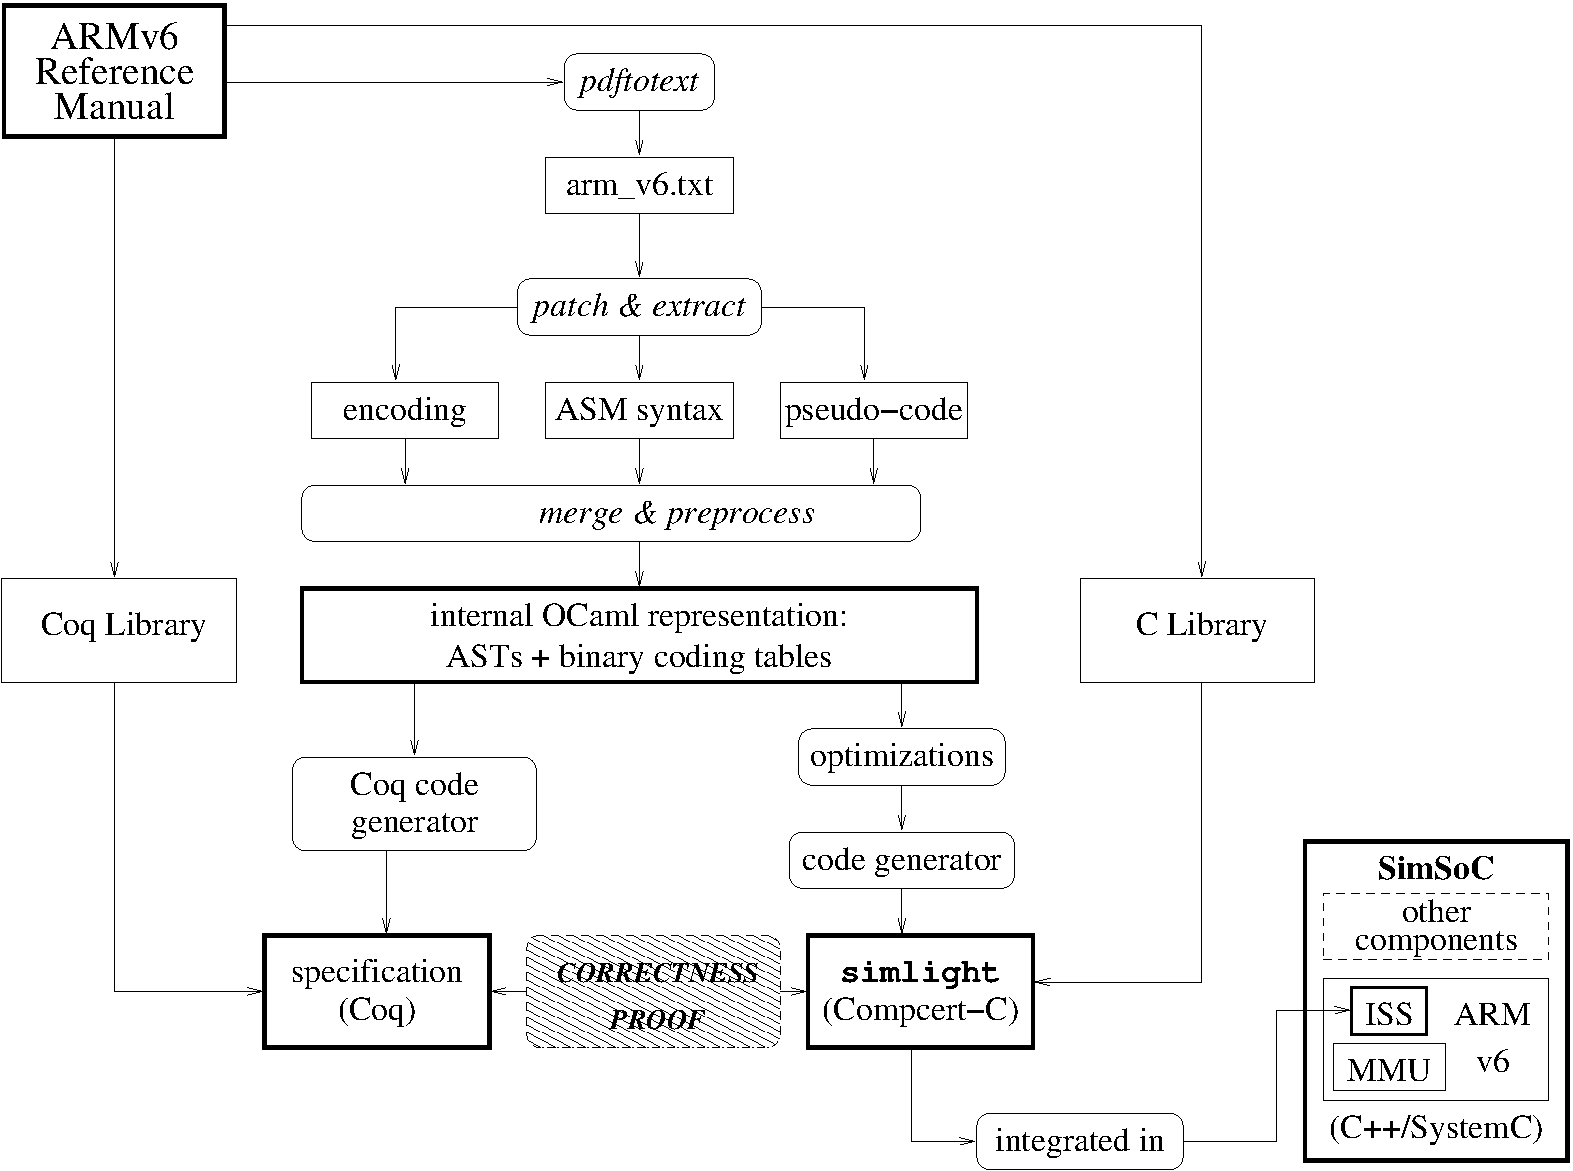
\includegraphics[width=\linewidth]{fig/fullarchi.pdf}
\caption{Overall generation chain}
\label{fig:arch}
\end{figure}

The overall architecture of the automatic generator is given in figure
\ref{fig:arch}.
% % JF -> XM: the text commented out here is redundant at this point.
% The requirement of \simsoc, the simulator, is to take the new architecture ARMv6
% into account, to prove such ARMv6 simulator is correct and the C simulator
% behavior fully corresponding to the document,
% and then integrate the proved correct simulator into \simsoc.
% Our idea is to first have a formal model of ARMv6 simulator including the ISS,
% a main processor, a simple memory model, a decoder, and a simulation loop.
% Then we compare the formal model with the C specifications of the simulator.
% This idea will be detailed in Section \ref{sec:gi}.
% Then the first task to do is to formalize the ARMv6 model in Coq
% ~\cite{coqmanual}. 
% Both formal specification in Coq and C description are relied on ARMv6 Reference
% Manual which
% contains 28500 lines.
% To have so many contents formalized by hand will be a tedious and error-prone
% work.
% We notice that the reference is basically written in natural language,
% but some parts are in pseudo-formal descriptions. 
% Then it is possible for us to automatically parse and manipulate them.
% The following introduces this automatic code generation.

The figure shows there are three data flows coming from manual.
Two are going to be formalized manually; the other one part
is going be interpreted and merged automatically.
%
% % JF->XM: no need for the next sentence..
% The reference is manually written.
%
% % JF->XM: dangerous to say the following this way: all our work could be compromized...
% which is not completely correct in any sense.
% We have found several bugs in the document by reading and by testing the 
% generated simulator.

More specifically, we can see the data flow from ARMv6 Reference Manual 
to the Coq model and to the simulation code. 
Some patches are needed from the textual version of the
reference manual because the latter contains some minor bugs
(see below).

Three kinds of
information are extracted for each ARM operation: its binary encoding format,
the corresponding assembly syntax, and its body, which is an algorithm operating
on various data structures representing the state of an ARM: registers, memory,
etc., according to the fields of the operation considered. This algorithm may 
call general purpose functions defined elsewhere in the manual, for which we provide
a \compcert C library to be used by the simulator and a Coq library defining
their semantics. The latter relies on Integers.v and Coqlib.v from the \compcert
library which allows us, for instance, to manipulate 32-bits representations of
words. The result is a set of abstract syntax trees (ASTs) and binary coding
tables. These ASTs follow the structure of the (not formally defined) 
pseudo-code. 

In the end, three files are generated: a Coq file specifying the behavior of all
operations (using the aforementioned Coq library), a \compcert C file to be
linked with other components of \simsoc (each instruction can also be executed
in stand-alone mode, for test purposes for instance)
and a Coq files representing each instructions in \compcert C AST
to be used for correctness proof.

% % JF-> XM: irrelevant subsection title
% \subsection{A reusable development framework}

% % JF->XM: redundant
% The back-end automatic code generator is shown in Figure~\ref{fig:arch}.
%input

\section{Analysis of the ARM reference manual}

The whole process starts with the ARMv6 reference manual {\stt ARM DDI 0100I}
\cite{arm6refman}. 
% % JF->XM, about next sentence: 
% % in a thesis, we are interested in the conclusions, what you get at then end,
% % and not in the process of getting it (unless it is a thesis on psychology
% We go through the manual roughly. 
The relevant chapters for us are:
\begin{itemize}
\item
\texttt{Programmer's Model} introduces the main features in ARMv6 architecture,
the data types, registers, exceptions, etc;
\item
\texttt{The ARM Instruction Set} 
explains the instruction encoding in general and puts the instructions in
categories;
\item
\texttt{ARM Instructions} lists all the ARM instructions in ARMv6 architecture
in alphabetical order and \texttt{ARM Addressing modes} gives all the five kinds 
of addressing modes;
\item
\texttt{Glossary} gives all the definitions of key words in ARMv6. We use it
as a reference to define manually the common functions.
\end{itemize}

% % JF->XM, about next sentence: 
% % in a thesis, we are interested in the conclusions, what you get at then end,
% % and not in the process of getting it (unless it is a thesis on psychology
% Then let us look carefully into Chapter \texttt{ARM Instructions} 
% in the reference manual. 

There are 147 ARM instructions in the ARMv6 architecture. 
For each instruction, the manual gives its encoding
table, its syntax, a piece of pseudo-code explaining its own
operation, its exceptions, usage, and notes.  Except the semi-formal
pseudo-code, everything else is written in nature language. 

% % JF->XM: not useful in this chapter
% An example of pseudo-code of instruction ADC is in figure~\ref{fig:adcpc}.

%preparing
% % JF->XM, about next sentence: 
% % in a thesis, we are interested in the conclusions, what you get at then end,
% % and not in the process of getting it (unless it is a thesis on psychology
% Using Linux command {\stt pdftotext} we are able to obtain a 28,500 lines 
% text file from the original pdf reference manual.

The first step is extraction and patching. 
We extract three files from the reference manual: 
a 2100 lines file containing the pseudo-code, a 800 lines file
containing the binary encoding tables, and a 500 lines file containing the
ASM syntax. 
Other than these three extracted files, there are still useful information left
in the document which cannot be automatically extracted.
% % JF->XM, about next sentence: 
% % in a thesis, we are interested in the conclusions, what you get at then end,
% % and not in the process of getting it (unless it is a thesis on psychology
% These informally described part will be later written by hand.
%
This is the case for
the arithmetic functions given in chapter \texttt{Glossary},
and for
the validity constraints information required by the decoder generator.
The corresponding information is manually translated into
a 300 lines OCaml file.

Before extraction, a patch is necessary for the main text file. This
patch is obtained from reading the manual or feedback from the generation result.
The patch fixes the mistakes in the original document, such as misspelling
function names, unclosed parenthesis, missing line, etc.
Most of these bugs were found by running the generator or
testing the generated simulator.
The differences are kept in a diff file,
so that they could be submitted to the ARM company and confirmed.

%preprocessing
Then each extracted file is parsed with the corresponding parser.
The one to parse pseudo-code is more complicated. Two preliminary phases solve
issues related to line breaks and indentation, given that indentation defines
the blocks in Python-like way. 

Then, a classical lexer parser combination builds the abstract syntax trees (ASTs). 
We have built our own ASTs for intermediate representation which contains the
elements representing both instructions and their addressing mode.

\section{Intermediate representation}

% \jf{Give here the main datatypes of the 
% ``internal OCaml representation, AST + binary code'' mentioned in 
% Figure~\ref{fig:arch}
% with a few comments on these}

The abstract syntax of the intermediate representation expressions
is given in Figure~\ref{fig:irexp}.
The corresponding OCaml definition is an inductive data type.
The type of expression supports numbers in different bases,
conditional expressions, function calls, binary operations, 
ranges (e.g. Rn[31:0] indicate the range of bits 0 to 31 of register Rn),
and the particular expression of ARM registers 
(e.g. \texttt{CPSR}, \texttt{SPSR}, and \texttt{Reg}), memory and coprocessor.
Additionally, two key words are included:
\texttt{Unaffected} which indicates the item is
not changed by an operation,
and \texttt{Unpredictable\_exp} which represents an unreliable instructions result.
The evaluation of expression \texttt{Unpredicatable\_exp} and \texttt{Coproc\_exp}
can bring side-effect. 

\begin{figure}
\begin{alltt}
  \textit{exp} ::= num
        | bin
        | hex
        | float
        | if \textit{exp} then \textit{exp} else \textit{exp} 
        | fun (\textit{exp list})
        | \textit{exp} binop \textit{exp}
        | \textbf{CPSR}
        | \textbf{SPSR} \textit{mode option}
        | \textbf{Reg} \textit{mode option}
        | var
        | \textit{exp} of \textit{range}
        | \textbf{Unaffected}
        | \textbf{Unpredictable\_exp}
        | \textbf{Memory} \textit{size}
        | \textbf{Coproc\_exp} \textit{exp list}
  \textit{mode} ::= Fiq | Irq | Svc | Abt | Und | Usr | Sys
  \textit{range} ::= bit | flag | index
  \textit{size} ::= byte | half | word
\end{alltt}
\caption{The abstract syntax of intermediate representation expressions}
\label{fig:irexp}
\end{figure}

Figure~\ref{fig:irstm} defines the abstract syntax of instruction statements,
which is defined in type \textit{inst}.
The C-style structural statements are supported: blocks, assignments,
conditional statements, loops (while loop and for loop), assert, case, and return.
Special function calls related to processor and coprocessor are presented
individually.
Within statements, \texttt{Unpredictable} appears again.
In pseudo-code, \armrf{UNPREDICTABLE} is used as the expression of right value
in the assignment (e.g. \armrf{data = UNPREDICTABLE}), or as the statement of call to
the function (e.g. \armrf{if...then...else UNPREDICTABLE}).


\begin{figure}
\begin{alltt}
  \textit{inst} ::= block \textit{inst list}
         | let \textit{fun} (\textit{args}) = \textit{inst list}
         | \textbf{Unpredictable}
         | \textit{exp} = \textit{exp}
         | if (\textit{exp}) \textit{inst} \textit{inst option}
         | Proc_function \textit{exp list}
         | while (\textit{exp}) \textit{inst}
         | assert \textit{exp}
         | for (string) \textit{inst}
         | Coproc_function \textit{exp list}
         | case (\textit{exp}) \textit{inst list}
         | return \textit{exp}
\end{alltt}
\caption{The abstract syntax of intermediate representation statements}
\label{fig:irstm}
\end{figure}

\section{Code generation}
\label{sec:codegen}

On the formal specification side (left side of the generation chain in Figure~\ref{fig:arch}),
we directly use the ASTs for generating Coq code. 

% % JF->XM: I guess that this flattening makes another interesting difference
% % between \simlight and the Coq model.
% % E.g. for ADC, there are adressing modes?
% % Which one is taken?
% % Was it easy to deal with?
% % Or is is for \simlight 2 only???

% % XM -> JF : flattening is for \simlight 2 only.

For the generation of C source code, we can make an easy optimization to generated the 
second version of \simlight,
in order to improve the simulation speed:
as we mentioned in Section~\ref{sec:slv62},
\textit{flattening} is one way of improving the simulation performance.
We {\em flatten} some instructions with their addressing mode
%\margjf{1}{XM, see important comment in latex source}. 
When an instruction $A$ can be used in an addressing mode $B$,
the generation provides a combined instruction $AB$.
This simple optimization can make the generation steps shorter and the generated
code faster. And after flattening, the notions of addressing modes disappear.

This flattening step is achieved by four operations:
\begin{itemize}
\item
  Inlining the addressing mode to instruction operation code;
\item
  Appending the validity constraint information;
\item 
  Merging the encoding table of the instruction and addressing mode case
  (example in figure \ref{fig:flatten})
\item
  Merging the ASM syntax of the instruction and addressing mode case
\end{itemize}

%\hide{
%\newcommand{\jfdots}{$\ldots$}
\newcommand{\jfdots}{$.\,.\,.\,$}
\begin{figure*}\centering
\small
\begin{tabular}{|c|c|c|c|c|c|c|c|c|c|}
\multicolumn{10}{c}{\small\em (a) binary encoding of the {\stt ADC} instruction}\\
\hline
31 \jfdots 28 & 27 26 & 25 & 24 \dotfill 21 & 20 & 19 \jfdots 16 & 15 \jfdots 12 & \multicolumn{3}{c|}{11 \dotfill 0} \\\hline
\stt cond & \stt 0~0 & \stt I & \stt 0~1~0~1 & \stt S & \stt Rn & \stt Rd & \multicolumn{3}{c|}{\stt shifter\_operand} \\
\hline
% \multicolumn{10}{c}{~}\\
\multicolumn{10}{c}{\small\em \phantom{\LARGE I}(b) binary encoding of the ``logical shift left by immediate'' operand\phantom{\LARGE I}}\\
\hline
31 \jfdots 28 & 27 26 & 25 & 24 \dotfill 21 & 20 & 19 \jfdots 16 & 15 \jfdots 12 & 11 \dotfill 7 & 6 \jfdots 4 & 3 \jfdots 0 \\\hline
\stt cond & \stt 0~0 & \stt 0 & \stt opcode & \stt S & \stt Rn & \stt Rd & \stt shift\_imm & \stt 0~0~0 & \stt Rm \\
\hline
% \multicolumn{10}{c}{~}\\
\multicolumn{10}{c}{\small\em \phantom{\LARGE I}(a+b) resulting binary encoding of the flattened instruction\phantom{\LARGE I}}\\
\hline
31 \jfdots 28 & 27 26 & 25 & 24 \dotfill 21 & 20 & 19 \jfdots 16 & 15 \jfdots 12 & 11 \dotfill 7 & 6 \jfdots 4 & 3 \jfdots 0 \\\hline
\stt cond & \stt 0~0 & \stt 0 & \stt 0~1~0~1 & \stt S & \stt Rn & \stt Rd & \stt shift\_imm & \stt 0~0~0 & \stt Rm \\
\hline
\end{tabular}

\caption{Flattening the ADC instruction with the shift left by immediate operand}
\label{fig:flatten}
\end{figure*}
%}

There are some specific points for the pre-processing phase:
\begin{itemize}
\item
  We can have a \emph{base register write-back} specification, saying that
  the base register which is used in address calculation will be modified.
  We have this case when \armrf{Rd == Rn}.
  The result is \armrf{UNPREDICTABLE} if the base register is PC.
  The base register write-back is disabled in M2, M3, M4 addressing modes.
  %and replaces the expression of write-back to the end of the
  %operation due to the rule of write-back.
\item 
  Some functions are reshaped depending on the number of arguments
  and the operation performed on them.
  For example, \armrf{CarryFrom(a + b)} is replaced by \texttt{CarryFrom\_add2(a, b)},
  which indicates that the carry is calculated from the ``add'' of two arguments.
\item
  Some \textit{if} or nested \textit{if} expressions concern occur when there is
  at least one \armrf{UNPREDICTABLE} in the branches.
  They are merged by pre-processing in order to remove repetitive branches,
  so that we get
  at most one \armrf{UNPREDICTABLE} in a then-branch.
  
\end{itemize}

%code generating
% % JF-XM: not much information there, propose to remove it
% From the cleared up intermediate representation to the object code, the code
% generator is basically a mapping. 
% Actually, we use a generator only for parts that are related to the
% instruction list (255 entities described in a same way). Indeed, it is not worth
% using a generator for something that is not repetitive because the generator
% would be longer than the generated code.

\section{Formats for C code}

% \jf{Explain here what we discussed: 
% generate C code in textual or \compcert AST format.
% Pros and cons. 
% Parser and pretty-printer.
% May add a figure if time available?}

To detail the generation of C implementations,
we present a new Figure~\ref{fig:genc}.
In the first line, 
the C source code is generated directly from the optimized intermediate
representation, and then go through the C parser provided by \compcert 
and a C to
\compcert C interpretation. 
Both instructions and library are parsed into \compcert C ASTs.
This result is integrated into the ARM simulator in SimSoC.
The second line translates the intermediate representation AST
into \compcert C AST, and then pretty print into Coq representation and C code too.
From the AST translation, only the instructions are obtained.
The result in Coq representation is used in the correctness proofs.
By comparison,
the pretty printed C code and the \compcert code obtained from the C parser are
identical to each other. Parsing to \compcert C does not lose
any information, which means the subset of C, \compcert C, is large enough to
be fulfill the requirement of ARM instructions.

\begin{figure}
\hfil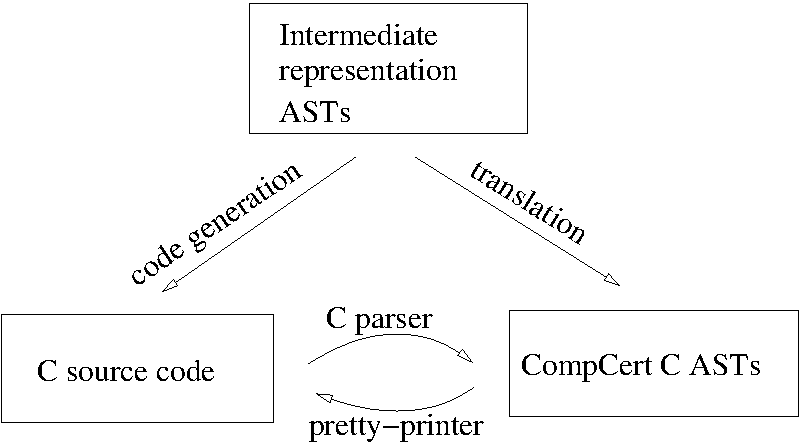
\includegraphics[width=0.7\linewidth]{fig/genc.pdf}
\caption{Generating C code}
\label{fig:genc}
\end{figure}

% \jf{Oh, starting on next Chapter, just saw the following in blue color, which
% I then moved from there to here -- it is a much better place.
% Note that the English (and the contents) of this blue text needs improvement.
% It contains part of what we discussed.
% Try to change/update it, using what follows.
% }

Proofs are to be performed on \compcert C ASTs, 
so the more direct way such ASTs are obtained, the better,
is in order to avoid possible mistaken auxiliary tranformations 
as far as we can
(no proofs have been performed on parsers and pretty-printers
for \compcert C).
But it makes sense only for automatically generated C programs:
writing ASTs by hand would be much too heavy and tedious.
Therefore, we have two cases to consider.
C libraries are written in textual format and parsed 
by the \compcert C front-end,
while C instructions automatically derived from the pseudo-code
are basically \compcert C ASTs
and pretty-printed for a manual double-check in a readable form.
As a result, for proofs,
the \compcert C parser is in the trusted code base (TCB) for libraries,
not for automatically derived code.
If we execute the corresponding programs using the \compcert C compiler,
the TCB is the same.
If we execute the corresponding programs using another compiler,
the TCB includes the pretty-printer and this compiler as well.

As a final remark on the reliability of the \compcert C parser
and the pretty-printer,
we also checked that, for all the generated code,
parsing then pretty-printing yields the original code.

\section{Mistakes in the ARM reference manual }

%% JF -> Vania : TODO : ENGLISH TO BE POLISHED IN THIS SECTION

While building the generators described in this chapter,
we discovered
several bugs in reference manual.

\begin{itemize}
\item
  Important lines were missing in instructions pseudo-code. In the
  operation of many conditional instructions, the condition checking
  was ignored. This leads to a fatal error when the execution
  condition is not satisfied.
  Also for some of load/store instruction, reading the base
  \texttt{address} is missing, which should be the content of register
  \texttt{Rn}. Without initialization, it is impossible to give
  \texttt{address} a value to start with.
\item
  The case sensitivity gave the same spelling different meanings.  
  For example, in the formal model, the binary operation $and$ applies to type
  Boolean, but operation $\mathit{AND}$ in capital is of type $word
  \rightarrow word \rightarrow word$.  Mixing two of them will lead to
  a type mismatch.
\item
  Information was lacking in keywords. For example, in general,
  \texttt{SignExtend} propagates the sign bit of its argument to 32
  bits, but for instruction \texttt{BLX(1)}, \texttt{SignExtend}
  is for the 24-bit signed to 30 bits.
\item
  Mismatched parenthesis.
%% XM : TODO. Retrieve what I meant.
% \item
%   Using deanery notation for binary system.
\item
  Wrong order of expressions in some operations. 
\item 
  In assembly syntax, the expression of register content \texttt{Rx}
  had to be replaced by \texttt{<Rx>}.
\end{itemize}


These bugs have been reported to ARM group.
The feedback was that all these bugs are fixed in ARMv7 reference
manual. 
% Then the effort to change our framework for ARMv7 architecture would
% be not much. And by reading the new reference manual, the description
% of instruction set is much more formal and better structured.
% Thus, the pre-process and other remedial transformation steps can be
% avoided.x


% JF BEGIN MOVED FROM CHAP 2

% {\color{blue}
% \noindent
% \texttt{BEGIN to be moved and updated somewhere}

% % XM
% % When we want to obtain the \compcert C representation of ARMv6 model, 
% % there are two ways. First, use the \compcert C provided converter to generate \compcert
% % C code from \simlight C file, which is not a verified translation step in \compcert.
% % JF -> XM : warning, what you wrote was misunderstood
% % JF 
% The \compcert C representation of ARMv6 can be presented in two ways:
% in textual form or using an AST (Abstract Syntax Tree).

% Two options can then be considered.
% The first is to use the converter provided by \compcert C to generate \compcert 
% C code from \simlight C file, which is not a verified translation step in \compcert.
% Or, we translate from the ARM internal representation
% AST to \compcert C AST. 
% If we use the first method, the unsupported things above
% will not be controlled. The generated code may lose information without warning.
% So the second transformation is in use.
% The second transformation also has weakness. The ARM internal AST only contains the
% ISS model. The function body of library functions is not included,
% which means the generated code has no definition of these library functions.
% We have to add them manually, or improve the feature of the transformation by 
% invoking the former.
% Whichever transformation we choose, we have to give a fake main function.
% This is because our correctness proof takes each instruction operation as one program.
% To build a \compcert C program, we must have the main entry point in the global 
% environment.

% \noindent
% \texttt{END to be moved and updated somewhere}
% }

% JF END MOVED FROM CHAP 2


%%% Local Variables: 
%%% mode: latex
%%% TeX-master: "thesis"
%%% End:

\chapter{Correctness proofs}
\label{cpt:correct}

%\jf{Add some pieces of Coq and LTac code}
In this chapter we introduce the correctness proofs we have performed
for the ARMv6 instruction set simulator \simlight by using the operational semantics
of \compcert C.
This work can be also considered as a significant experiment on
proving C programs by using a formalized operational semantics of C.

\selectlanguage{french}
\section*{Résumé}

\begin{resume}
Ce chapitre est consacré aux preuves de correction que nous avons effectuées
pour \simlight, le simulateur de jeu d'instructions de l'ARMv6 de notre projet,
en utilisant la sémantique opérationnelle de \compcert C.
Ce travail peut également être considéré comme une expérience significative
de preuves de programmes C selon une approche basée sur la sémantique opérationnelle.

Essentiellement, nous avons à établir qu'un programme C représentant l'ARMv6
se comporte conformément au modèle Coq attendu,
qui est un système de transitions sur un état abstrait directment défini en Coq.
Le programme C, via la sémantique opérationnelle définie dans \compcert,
est lui même modélisé par un système de transitions sur un état en un sens plus concret,
qui est un modèle de la mémoire C (telle qu'elle est formalisée dans \compcert),
habitée par des structures de données indiquées dans le programme \simlight.
Bien que le programme C et le modèle Coq soient dérivés à partir des mêmes
données du manuel de référence, et que la chaîne de génération de ces deux objets
soit en partie partagée,
on voit que ces objets sont de nature très différente.
Le modèle Coq abstrait reste aussi simple que possible
de façon à respecter visiblement ce qui est énoncé dans le manuel de référence.
En revanche, l'état concret pour \simlight prend non seulement en compte
le modèle mémoire de \compcert C,
mais des structures de données C complexifiées par un souci d'optimisation.

Afin de comparer le comportement du système de transition abstrait dans le modèle Coq
et celui du système de transition concret correspondant à \simlight,
nous commençons par définir une projection de l'état concret verts l'état abstrait.
Nous pouvons alors énoncer, pour chaque instruction ARM,
un théorème principal schématise en figure~\ref{fig:theo}
(une version plus exacte est donnée plus loin en figure~\ref{fig:theoca}).

Le preuves s'effectuent alors en itérant l'analyse des hypothèses
représentant des transitions entre états mémoire concrets,
selon une relation appropriée de la sémantique opérationnelle à grand pas
de \compcert C.
La transition correspondant dans le modèle abstrait est représentée
plus simplement par calcul,
car dans le modèle Coq de l'ARMv6, les instructions sont représentées par des fonctions.
\end{resume}

\selectlanguage{english}

\section{General idea}
\label{sec:gi}

% \margxm{1}{Consider the work as the proof for simulator and the proof for general C code}

% JF->XM: "C specification" is improper. Use "C program" or "C implementation"

% % XM
% For the ARMv6 ISS model, we build a Coq model on one hand,
% on the other, we have a C model from the same ARMv6 AST representation
%
% % JF
For the ARMv6 Instruction Set Simulator \simlight,
we have to compare a Coq model with a C implementation
(see Section~\ref{sec:overall}).

% % XM
% The correctness proofs will be processed in Coq proof system.  But how
% to deal with two models in two languages.  \compcert helps to build a
% bridge between them.  The general idea is to use the \compcert defined
% C formal syntax and semantics, which are specialized in Coq
% system. From it, we can obtain again a C model in Coq again.  With these two
% representations in Coq, it is able to begin the correctness proof.
%
% % JF
In order to formally reason on the correctness of the second with relation to the first
in the Coq setting,
we need a formal model in Coq of the C implementation.
It is provided by \compcert,
which defines a operational semantics of C formalized in Coq.
The two Coq models to be compared are state transition systems.

% % XM
% Although these two representations come from the same AST, the results are quite
% isolated from each other.
% From the macro point of view, the Coq specification follows exactly ARMv6
% reference manual, and keeps everything as simple as possible.
% The C specification has more objectives to achieve
% because \simsoc is aimed to be a high speed simulator.
% So optimization and some complex type definitions are required during the model
% design phase.
%
% % JF
Note that a large part of these two models is automatically derived
from the same source,
that is, an AST representation of the pseudo-code for instructions
taken in the ARMv6 manual.
However, even for this part, it is far from obvious that the two models
behave the same.
They are actually quite different from each other.  % JF isolated -> different

Basically,
the Coq specification follows exactly ARMv6 reference manual,
and keeps everything as simple as possible.
whereas the C program has more objectives to achieve
because it is aimed to be a high speed simulator.
In particular,
states in the model of the C implementation are much more complex
not only because the memory model defined in \compcert is taken into account,
but also because of optimizations and design decisions in \simlight
targetting efficiency.
In more detail:
\begin{itemize}
\item
% % XM
% The different type system.
% % JF No, a type system is something else. You mean data types. Ask me next time
The C implementation uses a big \emph{struct} to express the
ARM processor state.
The model of the state is a complex Coq record type, including not only data fields
but also proofs to guaranteed access permission, next block pointer, etc.
This is detailed in Section~\ref{sec:proj}.
\item
In the Coq specification,
% % XM
% semantics is in definition
% %  JF
transitions are defined in a functional style,
whereas in the model of the C implementation, a relational style is used.
%\margjf{1}{I added some ideas here}%
In general, the relational style is more flexible but
functional definitions have some advantages:
reasoning steps can be replaced by computations;
existence and unicity of the result are automatically ensured.
However, the functional style is not always convenient or even possible.
It is the case here, where the transitions defined by the C implementation
are relations which happen to be functions.
This comes first from the operational semantics, which needs to be relation
for the sake of generality.
Furthermore in our case,
the kind of record type mentioned in the previous item
is too complex to execute calculation with it,
so it is
more convenient to describe the state transformation for memory with a relation.
%
% because it is the semantics designed just for our instruction simulation.
% And in this simplified simulator, it does not implement co-processor or other
% features to interrupt the instruction operation.
% After one instruction, the processor will always turn to a new state.
% Whereas \compcert defines the semantics for C language, it is
% % % XM
% % in relation.
% % %  JF -- anyway commented out and rewrote the whole parag
% defined in a relational style,
% That is because the compiler translation line is certified by proving the same behavior
% of input and output languages. This \textbf{behavior} is expressed by program
% termination.
%
% The following is moved ot the previous item
% And the memory state is a complex Coq record type, including not only data field
% but also proofs to guaranteed access permission, next block pointer, etc.
% This kind of record type is too complex to execute calculation with it, so it is
% more convenient to have relation to describe the state transformation for memory.
\item
The two semantics operates on very different states.
For the Coq specification,
reading or changing the value of the processor state or other related variables
is easy to express.
In the model of the program, the state is based on a complex memory model
and load and store functions are used for read/write operations%\margjf{1}{to be checked by XM}.
% % XM original
% Two semantics operates on different memory systems.
% For Coq specification, semantics directly operates on processor state and
% other related variables. The value of these variables can be easily read or
% changed. However, the C semantics is based on the model of a whole memory used by
% compiler.
% The semantics, such as evaluation of statements and expressions,
% is described by a relation between initial and final memory state.
% Then, to get value of processor state or any variable, we need to load and store
% from memory state model.
\end{itemize}

\begin{figure}
\hfil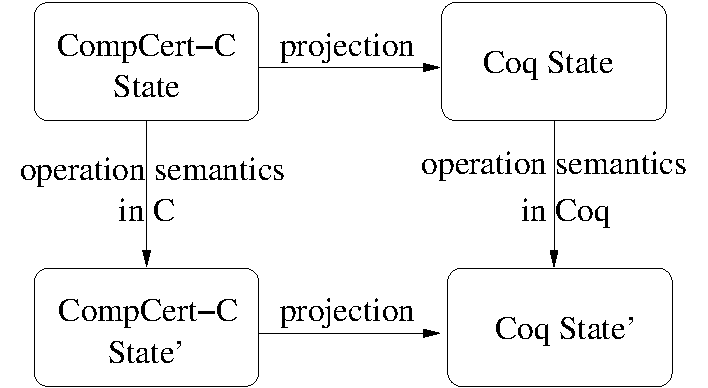
\includegraphics[width=.75\linewidth]{fig/theorem.pdf}

\caption{Main theorem for a given ARM instruction}
\label{fig:theo}
\end{figure}

For a given operation,
we state and proof
a main theorem which can be displayed by the diagram in Figure~\ref{fig:theo}.
On both sides, the execution of an instruction is described by a state transition.
% % XM (removed by JF, contents-free)
% From executing one instruction, the processor state will turn into
% a new state.
For the two ISS representations, ``State'' refers to the full description of
the system.
We start from a C memory state corresponding to
a more abstract state described by the Coq specification.
This correspondance is expressed by a projection relating the two models
of the state.
Then, executing the same instruction
on two sides will produce a pair of new processor states
which are related by the same correspondance.
Informally,
executing the same instruction on a pair equivalent states
will produce a pair of equivalent states.
%
% % XM Original
% if we have a pair of equivalent processor state, executing the same instruction
% on two sides will produce a pair of new processor state, which are equivalent
% again.
% Then we say, the C model has an instruction operates exactly like the
% formal model, and it is proved correct.

% \subsection{\compcert library}

% The \compcert library can be discussed in two parts.
% First is a collection for often used operation in Coq definitions and proofs.
% There are definitions and theorems about type \texttt{positive}, \texttt{Z},
% \texttt{nat} and conversion among them. Definitions and proofs on option
% type, list, boolean and etc.
% The second is the definitions on machine integers, and bitwise operations.
% It is based on Coq integer \texttt{Z}, and a proof to guaranteed the value is under
% the range from 0 to modulus.
% This module also support the conversion between type \texttt{Z}, \texttt{int} and
% \texttt{nat}.
% This can be extend to integers of size 8, 32 and 64 bits in our \emph{Bitvec}
% file.

% In \compcert, applicative finite maps are the main data structure used in
% memory state, global/local environment descriptions.
% There are two basic type, a \coqdocvar{Tree} and a \coqdocvar{Map},
% from them a number of maps and trees can be derived.
% The difference between the two is:
% For \coqdocvar{Tree} the return of $\langle get\rangle$ operation is an option type, if there is no
% data associated with key \coqdocvar{None} is returned. For \coqdocvar{Map} $\langle get\rangle$
% always returns data. If there is no data associated, a default value will be returned which is
% given since initialisation time.
% They two are both based on the abstract signature radix-2 search tree.
% And the derived trees and maps are named by their keys which can be integer or positive.
% The \coqdocvar{Tree} is used to define global and local environment which gathers memory
% information, maps the reference identifier to data information. Since the environment is built
% due to the memory contents, you can't get any information if you ask for a nonexistent address.
% On the contrary, memory content uses \coqdocvar{Map} indexed by integer. If a block
% in memory has not been allocated, it should return a default value \coqdocvar{Undefined} by
% any visit.

% %Applicative finite maps are the main data structure used in this
% %  project.  A finite map associates data to keys.  The two main operations
% %  are [set k d m], which returns a map identical to [m] except that [d]
% %  is associated to [k], and [get k m] which returns the data associated
% %  to key [k] in map [m].  In this library, we distinguish two kinds of maps:
% %- Trees: the [get] operation returns an option type, either [None]
% %  if no data is associated to the key, or [Some d] otherwise.
% %- Maps: the [get] operation always returns a data.  If no data was explicitly
% %  associated with the key, a default data provided at map initialisation time
% %  is returned.
% %
% %  In this library, we provide efficient implementations of trees and
% %  maps whose keys range over the type [positive] of binary positive
% %  integers or any type that can be injected into [positive].  The
% %  implementation is based on radix-2 search trees (uncompressed
% %  Patricia trees) and guarantees logarithmic-time operations.  An
% %  inefficient implementation of maps as functions is also provided.



% \subsection{\compcert C semantics}
% \label{sec:ccc}
% \compcert C is a large subset of C language.
% There are several things that is not supported by this subset.
% \begin{itemize}
% \item Types: it supports most of the types in C90 \cite{C90},
%   except the following points.
%   \begin{enumerate}
%   \item Unprototyped function type $(int f())$
%     and function type with variable number of arguments $(int f(...))$.
%     But it is possible to declare (not define) an external function of
%     the latter.
%   \item A structure can' have an unknown sized array type as the last
%     element. The size information must be known.
%   \end{enumerate}
% \item Wide char and wide string.
% \item Type cast do not support pointer to float.
% %\item The in-memory representation of pointer is opaque, can only be examined by
% %  a 32bits word.
% \item Specify bit fields in unions are not supported.
% \item In-line assembly is not supported.
% \item For the switch statement, \texttt{case} and \texttt{default} must appear.
%   And the \texttt{default} must occur at last.
% \item The only available external functions are printf, malloc, free,
%   \_\_builtin\_annot and \_\_bultin\_annot\_val. The other external functions can be
% declared but not implemented. One external function will generate a event trace.
% It says the result of the external function is computed by operating system,
% not the \compcert C code.
% \item Every program must has a \texttt{main} function declared.
% \end{itemize}


% When we want to obtain the \compcert C representation of ARMv6 model, there are
% two ways. First, use the \compcert C provide converter to generate \compcert
% C code from \simlight C file, this is not a verified translation step in \compcert.
% Or, we translate from the ARM internal representation
% AST to \compcert C AST.
% If we use the first method, the unsupported things above
% will not be controlled. The generated code may lose information without warning.
% So the second transformation is in use.
% The second transformation also has weakness. The ARM internal AST only contain the
% ISS model. The function body of library functions are not included.
% It means, the generated code has no definition of these library functions.
% We have to add them manually, or improve the feature of the transformation by
% invoking the former.
% Whichever transformation we choose, we have to give a fake main function.
% Because our correctness proof takes each instruction operation as one program.
% To build a \compcert C program, we must have the main entry point in the global
% environment.

% The semantics definition has two aspects. One is in small-step strategy,
% the other is in big-step.
% In our case, the big-step semantics is enough for correctness proofs.

% \compcert C describes C semantics in their memory model.
% Statement and expression evaluation is deterministic.
% The evaluation is represent using relation for a better proof induction.
% %%Coq had better support for proof induction over relations than over function definitions
% The formal operational semantics is described as transition system
% on memory states.
% $$G,E~\vdash ~\langle\textrm{expressions}\rangle,~M~\overset{t}{\Rightarrow}~v,~M'$$
% Here G represents global environment of whole program, E is the local environment,
% M and M' are memory states and t is a trace of I/O events,
% then v is a returned value.
% In \compcert C, expressions can be categoried into 15 cases and we have 13 of them
% are used in our correctness proofs.
% Some of the expressions are similar to the one for Clight and are already listed
% in \compcert papers \cite{lerbla08}.
% In Fig.~\ref{fig:evalexpr}, the inference rules different from Clight is showed.
% \begin{figure}
% \begin{minipage}[b]{1\linewidth}
% \centering
% %\small

% %  eval_call: forall e m rf rargs ty t1 m1 rf' t2 m2 rargs' vf vargs
% %                       targs tres fd t3 m3 vres,
% %       eval_expr e m RV rf t1 m1 rf' -> eval_exprlist e m1 rargs t2 m2 rargs' ->
% %       eval_simple_rvalue ge e m2 rf' vf ->
% %       eval_simple_list ge e m2 rargs' targs vargs ->
% %       classify_fun (typeof rf) = fun_case_f targs tres ->
% %       Genv.find_funct ge vf = Some fd ->
% %       type_of_fundef fd = Tfunction targs tres ->
% %       eval_funcall m2 fd vargs t3 m3 vres ->
% %       eval_expr e m RV (Ecall rf rargs ty) (t1**t2**t3) m3 (Eval vres ty)
% $$\frac
% {\begin{array}{c}
% G,E\vdash rf~M~\overset{t1}{\Rightarrow}~rf',M1\qquad
% G,E\vdash rarg^*~M1~\overset{t2}{\Rightarrow}~rarg'^*,M2\\
% G,E\vdash M2~rf' \Rightarrow vf\qquad
% \texttt{find\_funct}~(G,vf)~=~\lfloor fd\rfloor\\
% \vdash M2~fd~varg^* \overset{t3}{\Rightarrow}vres,M3
% \end{array}
% }
% {G,E\vdash M~\langle\textrm{\texttt{Call}}\rangle\overset{t1**t2**t3}{\Longrightarrow}vres,M3}
% $$
% \end{minipage}

% \begin{minipage}[b]{1\linewidth}
% \centering
%    % eval_assign: forall e m l r ty t1 m1 l' t2 m2 r' b ofs v v' t3 m3,
%    %    eval_expr e m LV l t1 m1 l' -> eval_expr e m1 RV r t2 m2 r' ->
%    %    eval_simple_lvalue ge e m2 l' b ofs ->
%    %    eval_simple_rvalue ge e m2 r' v ->
%    %    sem_cast v (typeof r) (typeof l) = Some v' ->
%    %    assign_loc ge (typeof l) m2 b ofs v' t3 m3 ->
%    %    ty = typeof l ->
%    %    eval_expr e m RV (Eassign l r ty) (t1**t2**t3) m3 (Eval v' ty)
% $$\frac
% {\begin{array}{c}
% G,E\vdash l~M\overset{t1}{\Rightarrow}l',M1\qquad
% G,E\vdash r~M1\overset{t2}{\Rightarrow}r',M2\\
% G,E\vdash l'~M2\Rightarrow (b, ofs)\qquad
% G,E\vdash r'~M2\Rightarrow v\\
% cast(v,typeof(l),typeof(r))=~\lfloor v'\rfloor\\
% store (G,~typeof(l),~M2,~(b,ofs),~v)=~\lfloor M3\rfloor\\
% \end{array}
% }
% {G,E\vdash (l=r)~M\overset{t1**t2**t3}{\Longrightarrow}v',M3}
% $$
% \end{minipage}
% \caption{Rules of operational semantics of \compcert C}
% \label{fig:evalexpr}
% \end{figure}


% The first rule in Fig~\ref{fig:evalexpr} is for evaluating function call
% expression. The evaluation is quite different from the rule for Clight.
% Not only that Clight is side-effect free, but \compcert C separates memory state
% transformation from evaluating simple expressions in order to preserve memory
% state.
% A function call can be evaluated in three steps:
% evaluating the function reference by identifier \coqdocvar{rf} to get where it
% stores;\\
% evaluating the function arguments references \coqdocvar{rargs} to get their
% values;\\
% finding the function definition \coqdocvar{fd} in the environment;
% then evaluating function call using \coqdocvar{eval\_funcall}.

% The second rule in Fig~\ref{fig:evalexpr} is evaluation of assignement expression.
% For Clight semantics, assignement is not an expression but a statement
% because Clight only accepts pure expressions.



\section{The ARMv6 model in \compcert C}
\label{sec:arm_ccc}


% % XM [JF: I don't understand what you say here]
% The top level of a \compcert C model is \texttt{program}.
% Program is defined as a record of \texttt{functions} (list of functions),
% the program entry point \texttt{main}, and (\texttt{global\_variables}).
% % JF [I write soemthing which makes sense but may be wrong,
% %     I don't know this detail about \compcert]
A \compcert C program a list of functions, including
the program entry point called \texttt{main},
with global variables as parameters.
% % JF: irrelevant
% We put each instruction pseudo-code in its own file.
The transformation from pseudo-code AST to \compcert C AST
% % XM
% will treat every instruction as a program itself.
% % JF
produces a standalone program for each ARMv6 instruction.
Then each has its own correctness proof separately.
In the generated \compcert C file, program contains only one function which is
the instruction operation. Other invoked functions are not included
because the instruction pseudo-code AST has nothing but a reference name.
% % XM
% In order to have these internal called function bodies, we have to add them
% manually into the functions list of the corresponding program.
% % JF
Their bodies are then manually included.

Every function is composed by its return type, function parameters,
local variables, and the function body.
The function body is a sequence of statements made of
expressions.
% % XM
% \compcert has very detailed syntax about every component.
% According expression definition,
% % JF
In \compcert ASTs, constructs are very detailed.
%
Each expression and each statement is annotated with its own type.
% In a program, the same definition of type may appear several times.
In a program, the same type may appear several times.
In the raw output of an AST, large and repeated expressions for types
occur everywhere,
making \compcert ASTs much more verbose and space consuming than necessary
and very hard to read.
In order to solve this issue and, more generally, get a readable code,
the pretty printer for ASTs introduces auxiliary names for types
-- common subtypes are then shared --
and also uses special notations for most constructs expression.
%\margjf{2}{I think that this was contributed by Fred B and Fred Tuong, no? Yes}
The implementation of this part was contributed by Frédéric Blanqui and Frédéric Tuong.

% Orig XM
% The raw output AST has the type defined every time when it was used.
% This made some long type definition repeat frequently and code looks messy.
% And printed code of \compcert C in Coq is too long and hard to read.
% In order to have a readable code,
% the pretty print code also uses special notations
% to denote each expression, and is optimized to define only once
% those sharing types.

% Definition fun_internal_B :=
%   {| fn_return := void;
%      fn_params := [
% proc -: `*` typ_SLv6_Processor;
% L -: int8;
% cond -: int32;
% signed_immed_24 -: uint32];
%      fn_vars := [];
%      fn_body :=
% `if (call (\ConditionPassed`:T1) E[&((`*(\proc`:T2)`:T3)|cpsr`:T4)`:T5; \cond`:T6] T7)
% then `if ((\L`:T7)==(#1`:T6)`:T6)
% then (call (\set_reg`:T8) E[\proc`:T2; #14`:T6; (call (\address_of_next_instruction`:T9) E[\proc`:T2] T10)] T11)
% else skip;;
% (call (\set_pc_raw`:T12) E[\proc`:T2; (call (\reg`:T13) E[\proc`:T2; #15`:T6] T10)+((call (\SignExtend_30`:T14) E[\signed_immed_24`:T10] T10)<<(#2`:T6)`:T10)`:T10] T11)
% else skip |}.
As a result, the code for \compcert C ASTs of instructions becomes
reasonably readable,
as illustrated on the following example (the instruction \texttt{BL},
``Branch and Link'').

\begin{alltt}\small
Definition fun_internal_B :=
  \{|
    fn_return := void;
    fn_params := [
      proc -: `*` typ_SLv6_Processor;
      L -: int8;
      cond -: int32;
      signed_immed_24 -: uint32];
    fn_vars := [];
    fn_body :=\footnotesize
     `if (call (ConditionPassed`:T1) E[\&((`*(proc`:T2)`:T3)|cpsr`:T4)`:T5;cond`:T6] T7)
     then `if ((L`:T7)==(#1`:T6)`:T6)
     then (call (set_reg`:T8)
             E[proc`:T2; #14`:T6;
               (call (address_of_next_instruction`:T9) E[proc`:T2] T10)]
             T11)
     else skip;;
     (call (set_pc_raw`:T12)
       E[proc`:T2;
         (call (reg`:T13) E[proc`:T2; #15`:T6] T10)+
         ((call (SignExtend_30`:T14) E[signed_immed_24`:T10] T10)<<(#2`:T6)`:T10)`:T10]
       T11)
     else skip \small
  |\}.
\end{alltt}

\noindent
The textual version of this \compcert C code would be:
\begin{alltt}\small
void B(struct SLv6_Processor *proc,
    const bool L,
    const SLv6_Condition cond,
    const uint32_t signed_immed_24)
\{
  if (ConditionPassed(&proc->cpsr, cond)) \{
    if ((L == 1))
      set_reg(proc,14,address_of_next_instruction(proc));
    set_pc_raw(proc,(reg(proc,15) + (SignExtend_30(signed_immed_24) << 2)));
  \}
\}
\end{alltt}
% \begin{alltt}\small
% fun_internal_B
%   (* typ_SLv6_Processor; int8 L; int32 cond; uint32 signed_immed_24)
%   \{|
%     if ConditionPassed (*proc, cpsr, cond) then
%       if L == #1 thenset_reg (proc, address_of_next_instruction (proc));
%     set_pc_raw (proc, reg(proc, #15 + SignExtend (signed_immed) << #2));
%   |\}.
% \end{alltt}

Another issue about the generated code is that the identifiers of variables,
function names, and so on, have their own numerical values.
These identifiers are important
% % XM
% reference for finding memory blocks.
% % JF
for referencing memory blocks.
But for the same identifier, we may have different values in different
\compcert C programs
as in the current version, each instruction corresponds to one standalone program.
This makes it difficult to share lemmas on common library functions
used in several instructions.
Our solution to this issue is discussed below in Section~\ref{ssec:cf}.

\section{The projection}
\label{sec:proj}
% How can we say the two systems behave the same.

% JF -> XM: you can be more accurate, refer to previous figures and chapters!
% % XM
% Although we already have both the two representations in Coq,
% we still need a way to measure the equivalence.
% Then it is necessary to build projection of the key variable, processor state,
% presents all parts of observable state elements in ARMv6 architecture.
% % JF
The state of the ARMv6 is defined in our Coq model in Figure~\ref{fig:armst}.
For convenience we will call this state the \emph{abstract state}.
% JF -> XM: actually some Coq would be welcome shere on in Chap 3.
% I think that the full Coq model is too big, however you can show
% the top definitions and give the length of the whole.
On the other hand, the same state is represented in the Coq model
of \simlight by the \compcert memory model applied to
the data structure displayed in Figure~\ref{fig:procc}.
For convenience we will call this state the \emph{concrete state}.
In order to state correctness theorems on \simlight,
we need to relate these two Coq models.
To this effect, we define a projection
from the concrete state to the abstract state.

Our theorems are then more accurately schematized by Figure~\ref{fig:theoca}
than in Figure~\ref{fig:theo} above.

\begin{figure}
\hfil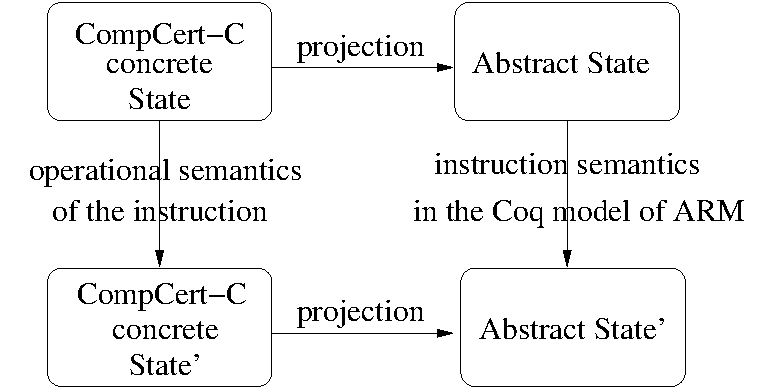
\includegraphics[width=.75\linewidth]{fig/theoremca.pdf}
\caption{More accurate theorem statement for a given ARM instruction}
\label{fig:theoca}
\end{figure}

Recall that our Coq model keeps everything as simple as possible and exactly
corresponds to the ARMv6 reference manual,
whereas the C representation is designed for high simulation speed.
Moreover, additional complexity is introduced because
a suitable memory model is required.

% % JF: useless now
% The projection is dealing with two different value storing systems.
% % JF: irrelevant
% On the right-hand side,
In the \compcert C model, variables are stored in the memory model.
This \compcert C memory model is detailed % "detailed" better than "complex" here
enough to describe the real memory properties,
but it is too complicated to use for computation.
\compcert handles another auxiliary parameter \emph{env},
the local environment.
It maps each variable identifier to its location and its type,
and its value is stored in the associated memory block.
% % JF: don't write this in written style, this is for oral explanations
% It helps us to find what we want in memory.
%
% JF->XM: for what follows I'm unsure to understand what you mean, pls check
% Messy original (your sentences NEVER start at column 0) is below
%\margjf{3}{XM please check}%
The value associated to a C variable or a parameter of a C function
is obtained by applying \texttt{load} to the suitable reference block in memory.
%
However,
this makes sense only after variable are allocated and initialized --
these two operations are performed when a function is called,
building a local environment \texttt{e} and an initialized memory state \texttt{m}.
Similarly, our projection makes sense only at this stage,
i.e., parameters representing the processor state are stored in memory.
Our Coq model of ARMv6 is of course much simpler
and computing the value of a component can be performed directly.

%  This \emph{env} is
% built from allocating function parameters and variables.  Then using
% \texttt{load} from the reference block in memory, we can have the
% value of requiring variable.  The projection is sound if and only if
% the variable allocation and initialization is finished. After these
% two processes, local environment \texttt{e} and an initialized memory
% state \texttt{m} will be constructed. And parameters like processor
% state now exist in memory.  In our own Coq model of ARMv6, we do not
% have such memory model. The variable can be got and computed directly.

% JF: material partly moved above.
% We built projection orientation form \compcert C to our Coq model.
% The two models have different representations of the key variable processor
% state.  Our Coq model keeps everything as simple as possible and exactly
% corresponds to the ARMv6 reference manual. The C model is designed to
% be more complex. Because it considers not only a complete
% representation of ARMv6 architecture but also a high simulation
% speed, optimization on type has been made.

The abstract state of the processor in our Coq model is a record.
It contains two records: one represents the main processor;
the other has the system control co-processor(\texttt{SCC})
and a simple ARMv6 memory altogether.
In the main processor record, the field \texttt{CPSR} (Current Program Status Register)
is defined as a word;
\texttt{SPSR} (Saved Program Status Register)
is a word depending on current processor mode;
\texttt{reg} maps the register to its value as a word;
\texttt{exn} is a list of possible exceptions, which is not in use yet.
\texttt{mode} is a numeration type for all processor modes.
In \texttt{SCC}, there are only two elements,
\texttt{reg} and \texttt{mem}:
\texttt{reg} is the register owned by \texttt{SCC},
which maps the register identical number to its word value;
\texttt{mem} is the ARMv6 memory model, which is a simple mapping from
address to word value.
% XM
% We do not have the MMU (Memory Management Unit) for the moment.
% JF (please check): anyway you had a contradiction with thee next sentence
% which speaks about MMU!
We only have a trivial MMU (Memory Management Unit) for the moment.

\sloppy
%\margjf{4}{I'm confused: the figure says cpsr, not CPSR, etc.}
The ARMv6 Processor data structure in C is given in Figure~\ref{fig:procc}.
It is a \emph{struct}  with thirteen fields,
which in turn contains three \emph{struct}:
\texttt{SLv6\_MMU},
\texttt{SLv6\_StatusRegister} for \texttt{cpsr},
and \texttt{SLv6\_SystemCoproc},
an array of \emph{struct} \texttt{SLv6\_StatusRegister} for \texttt{spsrs},
and six arrays for registers under each processor mode.
The other three are:
an identifier \texttt{id},
which is used when an embedded system has a multi-core architecture;
a pointer \texttt{pc},
which points to the fifteenth of register array under user mode;
and a boolean \texttt{jump} for expressing that the last instruction modifies
the \texttt{pc}, to be cleared after each cycle.
% Oral style
% Let us go back to look at the \emph{struct} \texttt{SLv6\_StatusRegister}.
The \emph{struct} \texttt{SLv6\_StatusRegister}
describes the status register, with bits represented as byte fields,
plus one field to identify the current processor mode.
The datatypes \texttt{CPSR} and \texttt{SPSRS} use this type.
The difference is that not every processor mode has \texttt{SPSRS}.
So an array for \texttt{SPSR} is used under every possible processor mode.
\fussy

% % JF->XM: commented out because not so useful/right/relevant. We can discuss.
%
% To have a complex types can make it much more efficient to reach the
% frequently used data field.  For example, the value of \texttt{CPSR} is a 32
% bits word in our Coq model, but in \compcert C model, it is defined as
% a structure, every significant bit is a field.  In instruction
% operations, it often discusses whether a bit, like \texttt{Nflag} in
% \texttt{CPSR}, is set or not. Then it is easier to get a bit value than
% calculate from a word.  There are more cases like this in C model of
% ARMv6. So the processor data structure is much more complex.  The
% projection has to be defined first for every module that we have in
% processor state of C, and then together they form the whole processor
% state of formal model.

% % JF->XM: Most contents here is trivial or chatting.
% % More useful : give some code of the projection

% \jf{Some code of the projection + comments.
% In particular, comment a little bit on \texttt{load}
% Refer to Fogure~\ref{fig:proj}.
% }

The top definition of the projection is shown below.
Each sub projection refers to the link between
an concrete element and its abstract version,
in red color in Figure~\ref{fig:proj}.

\begin{alltt}
Definition proc_proj (m:Mem.mem) (e:env):Arm6_State.state:=
  Arm6_State.mk_state
    (Arm6_Proc.mk_state
       (cpsr_proj m e)
       (spsr_proj m e)
       (regs_proj m e)
       nil
       (mode_proj m e))
    (Arm6_SCC.mk_state
       (screg_proj m e)
       (mem_proj m e)).
\end{alltt}

For example, the projection for registers owned by the main processor is
called \texttt{regs\_proj},
which takes the C memory state \texttt{m} and the local environment
\texttt{e} as arguments and return \texttt{register -> word}.
The definition is as follow:

\begin{alltt}
Definition regs_proj (m:Mem.mem) (e:env): register -> word :=
  let load_reg id n m e:=
    match find_reg m e id with
      | Some(Vptr b ofs)=>
        load_val (Mem.loadv Mint32 m (Vptr b (add ofs (repr n))))
      | _ =>Int.zero
    end in
    fun r =>
      match r with
        | R k => load_reg user_regs k m e
        | R_svc k _=> load_reg svc_regs k m e
        | R_abt k _=> load_reg abt_regs k m e
        | R_und k _=> load_reg und_regs k m e
        | R_irq k _=> load_reg irq_regs k m e
        | R_fiq k _=> load_reg fiq_regs k m e
      end.
\end{alltt}

Using the name of the register group as index to find the associated
memory block, from which the value is loaded.
Loading from memory state requires also the chunk information of its
type, size and signedness, and the offset.
In this case, the chunk of register is \texttt{Mint32} which means
it is 32-bit integer.
If the corresponding register is not found in memory state,
it returns zero. Initially, the value stored in register is zero.

According to the type of the argument on the right hand side of the
projection, the definitions of projections are quite different.
For example, the projection of a register given above
performs a case analysis on a value of type \texttt{register},
whereas the projection of SPSR depends on the type of exception modes.
We define a specific projection for each type.
Coq is rich enough to allow us to define a general projection
for all types of elements,
using dependent types.
However the gain in clarity of the specification is unclear,
and it would anyway be just a wrapper around specific projections,
so we did not build general protection for parameters.
For improving readability of the statement,
we even chose to define a projection relation for each instance.
For example, the projection relation of register Rn is :

\begin{alltt}
Definition rn_related (m:Mem.mem) (e:env) (rn:regnum):Prop :=
  reg_proj m e n = rn.
\end{alltt}



% To express the projection between the two representations of ARMv6 processor,
% we need two elements:
% the memory state where the variable is stored in the \compcert C model
% and the corresponding variables representation in formal model.
% Here we assume that in the \compcert C side,
% the memory is already allocated completely the variables of
% an instruction. Then the processor state and other parameters must
% exist in the current C memory state without doubt.
% So we can directly use the \coqdocvar{load} function to get the content
% of given block, without considering the memory reading mode, or if the type
% of the variable is volatile.
% The only problem is that the processor state is a quite complex structure in
% C side. The loading operation could not be simple and flat, and always
% contents more than one level loading for a data field.
% We have to first be very careful and with fully understanding of the
% C data structure to be sure that this manually written interactive with
% memory will not be error-prone.
%
% According to the definition in Coq formal model, processor state describes
% the instruction execution status in three conditions,
% \coqdocvar{Ok}, \coqdocvar{Ko}, and \coqdocvar{Todo}.
% Then there are three situations of projection for each corresponding Coq processor state.
% The state of formal model is detailed in Section~\ref{ssec:fsmoa}.
% So we are able to speak whatever happened in C ARMv6 model,
% we can find a corresponding state in the formal model.

\begin{figure}[h]
\hfil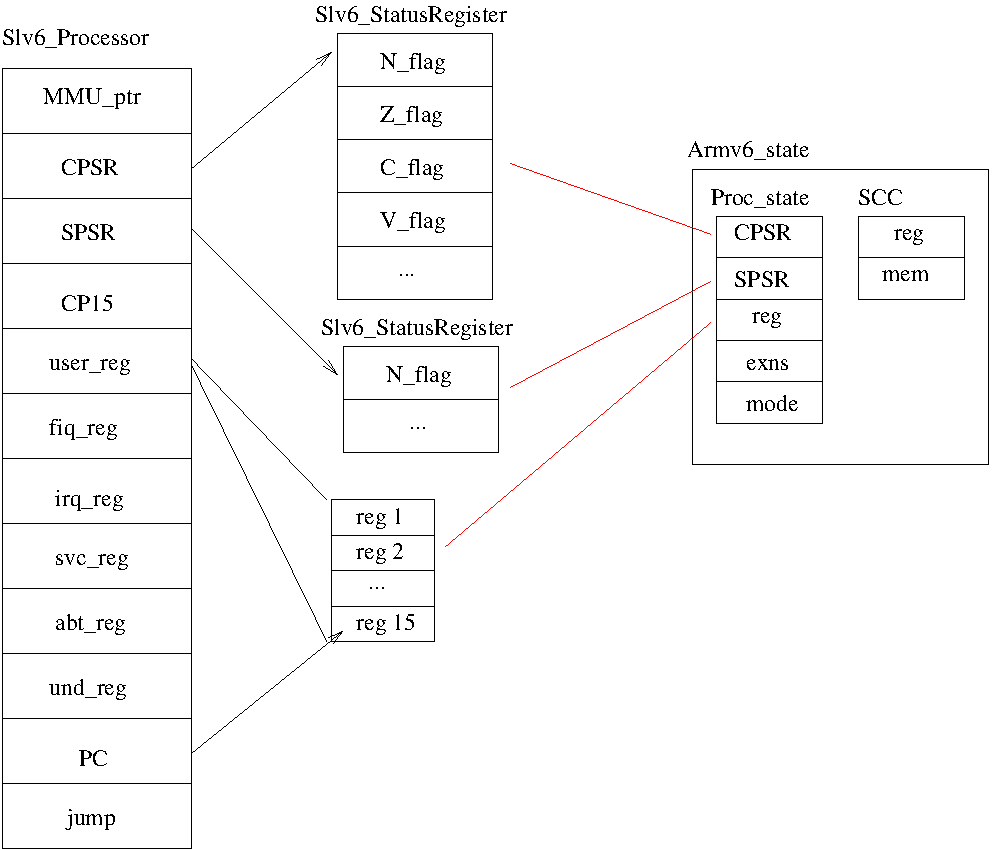
\includegraphics[width=.75\linewidth]{fig/projection.pdf}
\caption{Projection}
\label{fig:proj}
\end{figure}

\sloppy
% % JF -> XM: congratulations, your analysis sounds very good :)
In another project in our group called CCCBIP,
another way is used to express the projection.
The \texttt{eval\_expression} is reused to link the memory state
and the variable value:
$$G,E\vdash \texttt{eval\_expression}~(Ederef(Evalof(Evar x)))~M~\Rightarrow M,~v.$$
The value of $x$ in the formal model is $v$ and the \compcert C expression
$Ederef(Evalof(Evar x))$ is used
to dereference the variable $x$ from the memory contents.
In this case
the memory state remains the same because this evaluation only reads from memory.
This technique can be used there because the type of values are very simple
(integers).
On the contrary, the types in \simsoccert are much more complex:
we have structure pointers inside structures, or arrays of structures
inside structures, etc.
Simply dereferencing with $Ederef$ as in CCCBIP would raise issues in our case.
Manually writing such expression would become error-prone.
Even more, this method results in more inverting tactics during proving,
which makes the proof script harder to follow.
And after inverting, the function \texttt{load\_value\_of\_type}
(or \texttt{deref\_loc}), which loads from memory,
will be added to hypotheses as the premise of evaluating the right value of expression
\texttt{Evalof}.
And it is just the same as the \texttt{load} function with premises
on memory access mode predicate and type volatile judgment.
But these premises would then be redundant with the existing
hypotheses obtained during analyzing the evaluation of the expression
where the corresponding variable is mentioned.

\fussy

\section{Proofs}

\subsection{Proofs for an ARM instruction}
\label{ssec:prfinstr}

%%how many internal memory states


The correctness proof is based on the semantics of the formal model
and the \compcert C representation.
The semantics in the formalization is explained in Section~\ref{ssec:fsmoa}.
\compcert designed a semantics for \compcert C in both small-step and big-step.
The big-step inductive type for evaluating expression is enough for our proof.
The semantics is defined as a relation between an initial expression and an output
expression after evaluation.

% JF -> XM: don't chat.
% The first thing to do is to understand the semantics definition in \compcert.
As mentioned before, the semantics of \compcert C considers two environments.
The global environment \emph{genv} maps
global function identifiers, global variables identifiers to their blocks in memory,
and function pointers to a function definition body.
The local environment \emph{env} maps local variables
of a function to their memory blocks reference.
When the program starts its execution, \emph{genv} is built.
On the other hand, \emph{env} is built when
the associated function starts to allocate its variables.

% \noindent\jf{XM: I'm confused by the original paragraph
% so I propose something different and as short as possible,
% which may be wrong, pls check}.

To state the correctness theorem,
we compare a \compcert C function corresponding to
an ARM instruction with its formal definition in Coq.
% To state the correctness theorem,
% we choose to compare between a \compcert C function of
% instruction operation to its formal definition in Coq, instead of a whole program.
% That is because the execution of program discusses
% a \emph{state} that wraps current function,
% current statement, the continuation together with local environment, and memory state.
% The thing we want to discuss is if the projection still hold after executing one
% instruction.
% The value related to projection is just in memory.
% So the only valuable information is memory state who stores the variables we want
% to compare, and local environment helps us to find their memory address.
% % JF -> XM: distracting
% % And we do not need to discuss if the program terminated.
% So the \emph{state} contains too much information than we require,
% and it will bring difficulties to the
% correctness proof on things we do not need.
% The precise requirement is the memory
% state transition and evaluation of statement; in another word is executing the
% function body of instruction definition.
For such functions, it is enough to focus on the part of the concrete state
which is defined by the local environment.
We then consider a projection from the local environment to the abstract state
defined as follows.

\begin{alltt}
Inductive proc_state_related : Mem.mem -> env -> @result unit -> Prop :=
  | proc_state_related_ok :
      forall m e l b, proc_state_related m e
                        (Ok tt (mk_semstate l b (proc_proj m e)))
  | state_not_ok: forall e m mes, proc_state_related m e (Ko mes)
  | state_todo: forall e m mes, proc_state_related m e (Todo mes).
\end{alltt}

\noindent
The shape of the main theorem of an instruction is then:
\newcommand{\textmem}[1]{\textcolor{blue}{\texttt{#1}}}

\begin{alltt}
Theorem correctness\_instr:
  \(\forall\) e \textmem{m0} \textmem{m1} \textmem{m2} \textmem{mfin} vargs st other\_params out,
  alloc\_variables empty\_env \textmem{m0} (fun\_internal\_B.(fn\_params) ++
                                  fun\_internal\_B.(fn\_vars)) e \textmem{m1} ->
  bind\_parameters e \textmem{m1} fun\_internal\_B.(fn\_params) vargs \textmem{m2} ->
  (forall m ch b ofs, Mem.valid\_access m ch b ofs Readable) ->
  proc\_state\_related \textmem{m2} e (Ok tt (mk\_semstate nil true st)) ->
  other\_params\_related \textmem{m2} e other\_params ->
  exec\_stmt (Genv.globalenv prog\_bl) e \textmem{m2} fun\_internal\_B.(fn\_body)
                                       Events.E0 \textmem{mfin} out ->
  proc\_state\_related \textmem{mfin} e (S.instr\_step other_params
                              (mk\_semstate nil true st)).
\end{alltt}

\noindent
Let us explain it in more detail.
\begin{itemize}
\item
  In order to get the projection of the pair of original states, we need
  the following data: the initial memory state, the local
  environment, and the formal initial processor state.
  Recall that the projection is meaningful only after the C memory state
  is well prepared for evaluating the current function body.
  In the abstract Coq model, we directly use the processor
  state \texttt{st}.
  But on the C side, the memory state must provide the
  contents of every parameter, especially the processor state.
  We also need to observe the modification of certain blocks of memory
  corresponding to local variables.
%  a complete local environment -- a map from identifiers to address.
  Therefore, on  \compcert C side, a memory state and a
  local environment is prepared using following two steps.
\begin{itemize}
\item Allocating function variables: from an empty local environment,
  all function parameters and local variables ara allocated into
  the memory state \textmem{m0}, yielding a new memory state
  \textmem{m1} and the local environment \texttt{e}.
\item
Initializing function parameters: using \texttt{bind\_parameters} to initialize
parameters with a list of argument values \texttt{vargs}, a new memory state
\textmem{m2} is created.
\end{itemize}
\item
Now we have all elements for the projection to make sense are ready.
As the most important parameter of instruction operation,
the projection is first applied to \textmem{m2},
and we expect to get the initial abstract processor state \texttt{st}.
\item
The projection is also used on the other instruction parameters.
\item
Then the body of the function is executed.
On the \compcert C side, this is performed using a call to \texttt{exec\_stmt},
yeilding a new memory state \textmem{mfin}.
On the abstract side, the new processor state is obtained using \texttt{instr\_step}.
\item
Finally, we claim that the projection from the concrete state \textmem{mfin}
should provide the latter abstract state.
Note that all projections are performed using the same local
environment \texttt{e}.
\end{itemize}

The proof is performed in a top-down manner. It follows the definition of the
instruction, analyzing the expression step by step.
% % JF->XM as far as I understand it seems not important.
% And one proof block focuses on single expression unit.
The function body is split into statements and then into expressions.

% % JF
When evaluating an expression, we search for two kinds of information.
One is how the memory state changes on \compcert C side; the other is
whether the results on the abstract and the concrete model are related
by the projection.
To this effect, we use six kind of lemmas.
% % XM
% To complete the proof for main theorem, lemmas are required. Lemmas
% that can be categorized in four kinds shown below.  When evaluating an
% expression, there are two things we want to know.
% One is how the memory state changes on \compcert C side;
% the other is what is the outcome result by evaluating an expression
% when two sides are equivalent.

% what is the outcome result by evaluating an expression when two sides are equivalent.

\begin{enumerate}
\item
\textit{Evaluating a \compcert expression with no modification on the memory state.}\\
Such a lemma only discusses the expression evaluation on \compcert C side, involving
with the C memory state changing issue.
Saying a memory state is not modified has two aspects:
one is that the memory contents are not modified; the other is that the memory access
permission is not changed.
For example,
evaluating the binary expression $Sbit~==~1$ returns
% a new memory state, which is equivalent to input memory state.
an unchanged memory state.
\begin{align*}
&\textrm{if}~~ G,E~\vdash \texttt{eval\_binop}_c~(Sbit~==~1),\:M~\xLongrightarrow{\varepsilon}~vres,\:M'\\
&\textrm{then}~~ M=M'.
\end{align*}
% \begin{itemize}
% \item
%   if $G,E~\vdash \texttt{eval\_binop}_c~(Sbit~==~1),~M\xLongrightarrow{\epsilon}vres,~M'$,
% \item
% then $M~=~M'$.
% \end{itemize}

In Coq syntax, the relation in premise is expressed with \texttt{eval\_binop},
a companion predicate of \texttt{exec\_stmt} above,
devoted to binary operations.
In this lemma and the following,
$E$ is the local environment, $G$ is the global environment
and $M$ is the memory state;
$\varepsilon$ is the empty event (\texttt{Events.E0} in Coq syntax);
usually $t$ is used to represent a series of system events; $vres$ is the result.
%$\texttt{eval\_binop}_c$ is the semantics of \compcert C for evaluating binary operation.

Here, $vres$ is not important.
% % JF->XM: useless (redundant)
% We want to prove that the memory state does not change and,
% if nothing change on the abstract side as well,
% the projection will hold again after performing the evaluation.
The evaluation is performed under environments $G$ and $E$.
Before evaluation, we are in memory state $M$.
With no event occurring, we get the next memory state $M'$.
The proof is easy. According to the definition of \texttt{eval\_binop},
an internal memory state will be introduced.\\
\begin{center}
$\dfrac
{G,E~\vdash a_1,M\Rightarrow M'~~~G,E~\vdash a_2,M'\Rightarrow M''
}
{G,E~\vdash (a_1~binop~a_2),M\Rightarrow~M''}$
\end{center}
% \begin{center}
% $G,E~\vdash a_1,M\Rightarrow M'~~~G,E~\vdash a_2,M'\Rightarrow M''$\\
% \line(1,0){220}\\
% $G,E~\vdash (a_1~binop~a_2),M\Rightarrow~M''$
% \end{center}
Now, in our example, expression $a_1$ is the value of $Sbit$
and $a_2$ is the constant value $1$.
By inverting the hypothesis of type \texttt{eval\_binop},
we obtain several new hypotheses,
including on the evaluation of the two subexpressions
and the introduction of an intermediate memory state $M''$.
Evaluating them has no change on the C memory state.
Then we have $M = M'' = M'$.

In more detail, from the \compcert C semantics definition, we know that,
evaluation of an expression will change the memory state if
the evaluation contains uses of \texttt{store\_value\_of\_type}
(in \compcert versions before 1.11),
which stores the value in memory at a given block reference
and memory chunk. %  of reference type. % JF complicated...
In \compcert-1.11,
the basic store function on memory is represented by
an inductive type \texttt{assign\_loc}
instead of \texttt{store\_value\_of\_type}.
Since \compcert version 1.11 introduces volatile memory access,
we have to determine whether the object type is volatile before storage,
and also type size in addition of the access mode.

\item
\textit{Result of the evaluation of an expression with no modification on the memory.}\\
Continuing the example above, we now discuss the result of evaluating
the binary operation $Sbit~==~1$ both in the abstract and the concrete model.
At the end of evaluation, a boolean value $true$ or $false$ should be returned.
% Now we consider both sides of the projection.
% %JF -> XM "projective variable" does not exist
% First, we need to find the pair of projective variable $Sbit$
in \compcert C model and Coq model,
using the projection definition we introduced in~\ref{sec:proj}.
% \jf{I think that arguments are missing for \texttt{parameter\_related}:
% I intuitively expect a memory, an environment,
% an identifier for the name of the parameter, say \texttt{sbit},
% and an expected value, say $Sbit$. Not sure of the font to use.
% Make a choice and be consistent with the use of fonts,
% it is important for understanding,
% and showing that you understand what you write.
% Give the definition of \texttt{parameter\_related}.
% It is probably better to do that earlier, with \texttt{proc\_related}
% in the previous subsection.}
%
\begin{align*}
&\textrm{if} ~ \texttt{Sbit\_related}~M~\texttt{Sbit},\\
&\textrm{and} ~ G,E~\vdash \texttt{eval\_rvalue\_binop}_c~(Sbit~==~1),M\Rightarrow~v,\\
&\textrm{then} ~ v=(Sbit~==~1)_{coq}
\end{align*}
%
Intuitively,
if the projection corresponding to the parameter \texttt{sbit} in the C program
yields the right information from the abstract state,
then the evaluation will return the same value both
in the abstract and in the concrete model.
Here, the expression is a so-called ``simple expression''
that always terminates in a deterministic way, and preserves the memory state.

To evaluate the value of simple expressions,
\compcert provides two other big-step relations \texttt{eval\_simple\_rvalue} and
\texttt{eval\_simple\_lvalue} for evaluating respectively their left and right values.
The rules have the following shape:
\[
\dfrac{
\begin{array}{l}
G,E~\vdash a_1,M\Rightarrow v_1 \quad G,E~\vdash a_2,M\Rightarrow v_2\\
\texttt{sem\_binary\_operation}(op,v_1,v_2,M)~=~v
\end{array}}
{G,E~\vdash (a_1~op~a_2),M\Rightarrow v}
\]
In order to evaluate the binary expression $a_1~op~a_2$,
the sub-expressions $a_1$ and $a_2$ are first evaluated,
and their respective results $v_1$ and $v_2$ are used
to compute the final result $v$.

\item
{\it Memory state changed by storage operation.}\\
As mentioned before, evaluating some expressions such as \texttt{eval\_assign}
can modify the memory state.
Then we need lemmas stating that corresponding variables in the abstract
and in the concrete model will evolve consistently.
For example, this is stated as follows for an assignment on register $Rn$.
Here we use the projection relation \texttt{register\_related}.

%\jf{Put the definition of \texttt{register\_related} in the previous section.}
% \jf{But again I don't understand: there should be an argument for the name of the register,
% say \texttt{n} or  \texttt{Rn}
% and another for the value contained in the abstract model, say $rn$;
% moreover $M$ is rightly changed in $M'$,
% but I would expect $v$ instead of $rn$ in the conclusion.}
\begin{align*}
&\textrm{if} ~~ \texttt{rn\_related}~M~rn\\
&\textrm{and}~~  G,E~\vdash \texttt{eval\_assign}_c~(rn:=rx),M~\Rightarrow~ M',v\\
&\textrm{then} ~~ \texttt{rn\_related}~M'~rn
\end{align*}

\item
\textit{Evaluating expressions with modification on the memory.}\\
This is similar to the previous case.
% This is one of the cases that the memory state is modified, some of the memory blocks
% represent fields of processor state is modified. And a new projection will be hold.

\item
\textit{Internal function call.}\\
% To deal with the internal function calls, our translated code is not enough.
Internal functions are described in an informal manner in the ARMv6 reference manual.
No pseudo-code is available for them,
which means that the corresponding library functions,
both in the abstract Coq model and in \simlight,
are written by hand.
In order to get a suitable \compcert C AST to reason about,
we use the parser provided in \compcert.
% The translated code is from pseudo-code AST to \compcert C AST and prints them into
% Coq representation, which only contains the definition of instruction operation.
% Then we have no definition on the library function. We have to either
% define them manually by reading the reference or reuse part of the \compcert
% compiler, the parser from normal C
% code to \compcert C AST, in order to obtain the function bodies from the
% hand-written C definition for library functions in \simlight.
% Then add them to the translated code.
When combining the simulation code of an instruction with the
code of library functions,
we need to take care of the memory allocation problem.
In \compcert C representation, identifiers are unique positive numbers
which indicate the memory block where corresponding variables are allocated.
Currently, the extra identifiers introduced by library functions are
added manually and assigned with fresh block numbers.
\label{page:libfunast}
% \jf{Something missing here to explain what is the problem with these numbers,
% and which processes can be automated in future work.}
% \xm{Both processes can be represented automatically.
% This can be a future work to be completed. }
%
\begin{align*}
&\textrm{if} ~~  \texttt{proc\_state\_related}~M~st\\
&\textrm{and} ~~ G,E~\vdash \texttt{eval\_funcall}_c~(copy\_StatusRegister)_c,M\Rightarrow~v,~M'\\
&\textrm{and} ~~ st'~=~(copy\_StatusRegister)_{coq}~st \\
&\textrm{then} ~~\texttt{proc\_state\_related}~M'~st'.
\end{align*}
% \begin{itemize}
% \item
% if $\texttt{proc\_state\_related}~M~st$,
% \item
%   and $G,E~\vdash \texttt{eval\_funcall}_c~(copy\_StatusRegister)_c,M\Rightarrow~v,~M'$,\\
%   and $st'~=~(copy\_StatusRegister)_{coq}~st$
% \item
% then $\texttt{proc\_state\_related}~M'~st'$.
% \end{itemize}

After an internal function is called, a new stack of blocks is
allocated in memory.
After the evaluation of the function is performed, these blocks will be freed.
Unfortunately, this cannot bring the memory back to the previous state:
the memory contents may stay the same,
but the \texttt{nextblock} pointer will skip these just freed blocks and point
to the followed block.
% \jf{What do you intend to say in the next sentence? That equal memories
% is too restrictive I guess?
% So what? Do you have a suitable ``equivalence'' predicate on memories?
% Seems that the answer is no.
% I guess that you just say that some observations on memory will
% provide the expected result.
% Is it right? And is it enough for performing the next proof steps,
% which may require resoning on many projections?}
% \xm{To state that two memory states are the same means that
% their memory contents, the memory access permission, the next block, and so
% on, should all be the same.}
For lemmas on evaluation of internal functions,
we can observe the returned result on variables and compare it
with the corresponding evaluation in the formal specification.
For example,
the lemma above is about the processor state after evaluating an internal
function call \texttt{copy\_StatusRegister} which reads the value of
CPSR and then assigns it to SPSR.
% It always follows the condition. JF->XM: which one? Seems redundant anyway.
The evaluation of \texttt{copy\_StatusRegister} should be protected by
a check on the current processor mode.
If it is neither system mode nor user mode,
the function \texttt{copy\_StatusRegister} can be called.
Otherwise, \simlight % the simulation system; JF->XM: correct? Yes.
will return ``unpredictable'' with an empty message.

% \texttt{copy\_StatusRegister} is defined differently in two side.
% Every time when we want to perform copying from CPSR to SPSR, we have to
% first check if current mode has SPSR. That means function
% \texttt{copy\_StatusRegister} always follows the condition judging which is
% the current processor mode, and if current mode does not have SPSR it will return
% an empty message.

Then we have to reason on the newly returned states,
which should still be related by the projection.
This step is easy to prove by calculation, simplifying on
two representations of the processor state.

% JF HERE
\item
\textit{External function call.}\\
% \jf{Question to XM:
% from what you say something is unclear to me:
% is it feasible to perform proofs, or just impossible?
% When you say that ``only few built-in external
% functions have their certain semantics'' (I'll rephrase)
% does it mean that \compcert provides an axiomatic
% description of these functions?
% And that the implementation in assembly code is proven
% correct wrt. these axioms?
% At the moment I write something else.
% Note that I'm NOT sure at all, I just GUESS.
% It seems better to distinguish external functions and external function calls.
% Please check.}\\
% Currently, we do not consider external function calls in C representation.
% Because \compcert C has not
% yet supported self defined external function calls, only few built-in external
% functions have their certain semantics. If we have an external function call in
% C code, the translated \compcert C representation will have an empty body for
% external function, containing only the input argument type and the returned value
% type.
% We can only reason about:
% External functions are not part of the \compcert C language.
% They only can be described in an axiomatic way.
The \compcert C AST of an external function call contains
the types of input arguments and of the returned value,
and an empty body.
\compcert provides the expected properties of a few
built-in external functions such as \texttt{printf},
\texttt{malloc} and \texttt{free}.
We proceed similarly for the external functions of \simlight.

% % JF: moved here this paragraph which was after the list
% In general, we expect the result returned by evaluation of external function.
% But there is no semantics provided on the self defined external function body.
% In \simlight, some functions are defined as external ones.
% This is for modularizing the simulator. %  to make it clean %% Of course!!
% Even it is a simplified version of the large \simsoc simulator,
% it is still a quite complex system.
% So the problem left for us is to either change all the external
% functions into internal or give assumptions every time we meet
% external.
%
% % JF Rewriting this paragraph, removing redundancies
% \jf{Email sent, check/rewrite according to answers.}
In \simlight, some functions are defined as external ones
-- something which is needed even is this simplified version of \simsoc.
They could be changed into internal functions in the future
but in the current version, they are left external.

The general expected properties of an external call are as follows.
\begin{itemize}
\item
  The call returns an result, which has to be related to the abstract.
\item
  The number of arguments must agree with the signature.
\item
  After the call, no memory blocks are invalidated.
\item
  The call does not increase the max access permission of any
  valid block.
\item
  The memory state can be modified only when the
  access permission of the call is the maximal.
\end{itemize}

% Currently, we can only give \texttt{Axiom} on external function about the execution
% result.
% According to the given property, evaluation of an external function will not change
% the original memory contents.
% Then it is better to return the execution result in a variable.
% The common \texttt{Axiom} looks like:
For \simlight, the result of an external call is written in a variable
such as \texttt{vres} in the next example.
A typical axiom for stating that the external function \texttt{ef\_c}
returns a result specified by the Coq expression \texttt{ef\_coq} is:
\begin{alltt}
Axiom res_extcall :
  forall m ef_{c} targs tres vargs t m' vres,
    eval_funcall m (External ef_{c} targs tres) vargs t m' vres ->
    vres = ef_{coq}.
\end{alltt}
%The result of executing function $ef$ on both sides will be the same.
\end{enumerate}

\subsection{Proof design}
% % JF -> XM: the following is about prof technique and currently obscure
% % therefore probably less important than the other on structuring into lemmas.
% % I moved it

%% JF->XM: this is well-known
% During the proof process, some proof strategies are frequently used.
% Repeating every time the same proving steps is repetitive and time consuming work.
% It is better to have lemmas on them.
% Or even we can define our own tactics to have these steps done in one move.
As usual, repetitive steps in proofs are dealt with using auxiliary lemmas and
dedicated tactic definitions.
In our case,
% most of this work is done for \compcert C side.
most of them are related to the semantics of \compcert C.
Indeed, since the abstract Coq model is defined in a functional style,
many proof steps are just reductions using, e.g., \texttt{simpl} or \texttt{unfold}.
% One reason is that semantics is defined in functional way in the formal model.
% The execution result can be carried out by simplifying or unfolding
% the functional definition.
In contrast, the execution of a C program is provided by a inductively defined
relations, the operational semantics.
Decomposing this execution step by step amounts to perform so-called \emph{inversions}
on hypotheses relating concrete memory states according to the operational semantics.
In practice, a large amount (several dozens) of inversions are performed,
bringing serious issues on space-time consumption and maintenability.
We studied a general solution to this problem, to
% But in \compcert side, to find a execution result we have to follow step by
% step the premises which are defined in the semantics inductive types.
% This means that there are really a lot of inversions on hypotheses.
% The issue on inversion brought us much inconvenience in our proof scripts,
% like scripts size, time consumption, naming issue.
% The way to improve the proof strategy will
be introduced in Chapter \ref{cpt:inv}.

More specifically,
back to the design of proofs,
here are the main issues and how they are dealt with.

%\begin{itemize}
\paragraph{Getting a usable local environment.}
% % JF: Seems to be useless
% The importance of parameter local environment is mentioned above.
%
We often need to consider whether a variable exists in C memory or not,
and to get the corresponding location in memory.
To this effect, the concrete contents of the local environment \texttt{e} is required.
To achieve this,
inversions are systematically performed on \texttt{alloc\_variables} hypotheses.
Then \texttt{e} becomes a \emph{closed} (and reduced)
mapping indexed by variable identifiers
(before, \texttt{e} is just a variable having the type of a mapping).
%
% % JF-> XM : your proving strategy is not defined (at least at this point)
% Through the proving strategy, we often consider whether a
% variable exist in C memory or not.  It is necessary to have a concrete
% mapping \textbf{e}. Then it is possible to look for variable locations
% in memory. To achieve this, the operation \texttt{alloc\_variables}
% has to be inverted for each argument of a function.
%
\paragraph{Finding a variable location in memory from its  identifier.}
This is simply solved by applying the \texttt{get} operation
provided by \compcert on the local environment~\texttt{e}.
This computation can actually be performed when~\texttt{e} is closed.
% Using the concrete local environment, it is possible to judge whether
% a variable reference has a corresponding location in memory or not.
%  It is simply using a get in tree structure with index.

\paragraph{Finding a function location in memory.}
Two kinds of functions exist in C.
Internal functions are in the local environment \texttt{e},
whereas external functions are in the global environment \texttt{g}.
When a function reference is met,
a \texttt{get} operation is invoked on \texttt{e},
then on \texttt{g} in case of failure.
% In C, there are two kinds of functions: internal functions and external
% functions.  When we meet a function reference, in order to know which
% kind it is, we have to look up into the local environment first. If it
% exists in the local environment, it is internal.  If not, we search it in
% the global environment. If it exists in global environment, it is
% external. Whether searching in local or global environment, it is to
% \texttt{get} from a special tree with a reference.

\paragraph{Evaluating memory states.}
\compcert C semantics operates on memory states.
% % XM
% To observe
% JF
Observing
them is essential, in particular to compare the concrete state with
the expected abstract state.
The memory state stays unchanged,
except when a \texttt{store} occurs during evaluation.
In the inductive relation \texttt{eval\_expr},
this only happens for an assignment (\texttt{eval\_assign}),
an assignment with arithmetic operation (\texttt{eval\_assignop})
or a post-increment operation (\texttt{eval\_postincr}).
% JF -> XM: the following is wrong (it is correct only for base cases)
% All the other expressions will not change the memory state.
Whatever the expression, it has to be analyzed and recursively decomposed
in order to get closed (then usable) memory states.
Again, this is performed using inversions on \texttt{eval\_expr} hypotheses.
The inductive type \texttt{eval\_expr} is big and expressions in
\simlight are complex,
raising serious issues with the Coq standard tactic \texttt{inversion}.
We then decided to write our own inversion tactic.
We go back to this in Section~\ref{sec:ninv}.

\paragraph{Analysing values in a memory block.}
The \compcert memory model includes four kinds of operations:
\texttt{load}, \texttt{store}, \texttt{alloc}, and \texttt{free}.
They operate on a memory chunk at a given address.
For these four operations, several properties are provided.
We use them to determine
which block or memory chunk is affected by one of these operations,
and which part of the memory is left unchanged.

%\end{itemize}

\subsection{Proofs for shared library functions}
\label{ssec:cf}

Every ARMv6 instruction contains one or more calls to
internal or external functions. For the moment, the external functions
are not taken into account, for a reason explained in ~\ref{ssec:ccc}.
As mentioned in Section~\ref{sec:arm_ccc},
% % JF: usure of the syntax and anyways, complicates the reading
% % By the way I don't like "instruction operation", looks improper English
% except the instruction operation body,
functions called in an instruction need to be added manually.
Most of these functions are used in different instructions.
% But the proposition we ask from them is mainly the same.
% % JF: remove or simplify the following which is obvious
% Adding them one by one into every instruction and
% having similar proofs everywhere is a rigid work.
% It is better to have their function body declared in a common file and have their
% lemmas shared by all related instructions.
As the properties expected from them are always the same,
we want to state and proof corresponding lemmas once for all.
%
% % JF-> XM: big issue here
% \jf{I'm not sure that you are right: as far as I understand,
% proofs are performed on different standalone programs:
% an independant program for each isntruction.
% As we have different programs, the fact that identifiers cannot
% be repeated is irrelevant, since it is relevant only
% inside a given program.
% Hoowever, I think that we have no control on the identifiers
% representing variable or function names.
% And this is enough to make function be represented by
% different identifiers in different programs,
% hence the issue and the solution with Coq modules.}

One issue from the \compcert compiler is that
% every identifier is a positive number which also
% indicates the location in memory.
% And identifiers cannot be repeated.
identifiers (positive numbers indicating a location in memory)
cannot be repeated:%\margjf{2}{To be changed if previous comment in red is correct}:
these memory locations are settled once a program is evaluated,
and the global environment and local environment will be
filled with allocation information.
% To add a function into a programs,
% we have to re-arrange the memory allocation by giving new blocks to
% the new introduced variables and functions.
The insertion of functions in a program is performed by the
assignment of new blocks to the corresponding identifiers.
The issue is that the same function in different program
will be represented by different identifiers.
We solve this issue using Coq \emph{sections}.
A section is defined for each function
with its associated lemmas.
Its variables are defined abstractly by just giving their types.
% When adopting library function module to a program,
% the assumed identifiers will be assigned to real values.
Integrating such a function into the \compcert code of an instruction
consists in importing the file containing the corresponding section,
instantiating additionally assumed variables with appropriate values,
then performing memory allocation.
% % JF: an adding function is a function for performing addition !!!
% This adding function needs to be done before allocating memory.

% % JF -> XM ??? A library function IS an internal function, no?
% How to perform proving on library function is like the proof for internal
% function, which is explained in Subsection~\ref{ssec:prfinstr}.
Proofs on library functions are performed in the same way as for instructions,
see Subsection~\ref{ssec:prfinstr}.

% In every ARMv6 instruction, operation contains calls to internal or
% external functions. For the moment the external functions are not take
% into count, the reason is explained in ~\ref{sec:ccc}.  We mention in
% previous section \ref{sec:arm_ccc}, except the instruction operation
% body, the other functions call in one instruction need to be added
% manually.  Most of these functions are used in different instructions.
% But the proposition we ask from them is mainly the same.  Adding them
% one by one into every instruction and having similar proofs everywhere
% is a rigid work.  It is better to have their function body declared in
% a common file and have their lemmas shared by all related
% instructions.  In practice, lemmas we stated for each internal
% function are about, whether it have side-effect, if so, the outputs
% should be the same in formal model and \compcert C model. Or some of
% the variable we want to reason about is not changed by such internal
% function.  And the proposition here depends on an abstract memory
% model.  We have to assume there is a block in a memory state refers to a
% definition of an internal function.  Then apply to each instruction,
% these block value will be instantiated according to the current memory model
% build by programs.

\subsection{Proofs on tricky operations on words}
%Except the lemmas on internal functions, there are other library functions about
%comparing the same function defined in different ways,
We also have lemmas for checking that different ways of computing
a function actually provide the same result.
An example is the function for getting the bit at a given position
in a word represented by a binary integer.
The equality to be proved is, after simplification:
\begin{alltt}
\hfil and (shru \(x\) (repr (Z\_of\_nat \(n\)))) (repr 1) = \(x\)\:[\(n\)].
\end{alltt}
It means that the definition of \texttt{get\_bit} used in \simlight
can be (efficiently) computed by a combination of binary operations
\texttt{and} and \texttt{shru} (logical shift right)
on the integer $x$ and the bit number $n$.
On the right hand side,
the formal specification uses a bit mask on the object integer $x$
to get the $n^{\rm th}$ bit.
The comparison is quite complicated due to the range of the result in type integer.
We have to take a restriction into account,
saying that $n$ should be greater than $0$ and less than the word size,
and to add specific lemmas on other arithmetic definitions.

\section{Tactics}
\label{sec:tactic}

Coq provides the Ltac language to allow the user to define her/his own tactics.
% % JF useless
% Like the built-in tactics, we can define our own tactics to apply to goals during Coq proofs.
LTac expressions can be used in the proof script of a given theorem, or in
% This process can be defined during proof or pre-defined as
a top-level Ltac definition.
The most useful
% semantics % JF->XM: Nothing to do with semantics
construct
of Ltac is the pattern matching on a proof goal,
which analyzes the current goal and binds names to useful informations.
This is used for our inversion \hcinv described in Section~\ref{sec:ninv}.
We also defined tactics dedicated to our specific needs,
% helping us to make the proofs easier and systematic.
representing systematic reasoning schemes on the \compcert C semantics.
Most of them deal with the C memory model and with operational semantics rules.
% we have many proof strategy repetitive.
% The most work we are dealing with through all the proof scripts
% is the C memory model and the operational expressions semantics.
% \begin{itemize}
% \item
\subsection{Load/store operations}
% The properties we have to discuss very frequently is
Many reasoning steps are about
the effect of a load/store operation on memory.
% The load/store operations are always bounded
% by the low/high bound of the memory blocks.
Such operations are always constrained by low and high bounds of the memory blocks.
In order to know
whether the memory block we focus on remains the same
or has been changed to a new contents,
we have to determine the range of blocks
% % JF I don't understand. You may mean what I write below
% operated on C memory model
targetted by operations on memory.
%
% % JF I don't understand. Is it related to the previous sentence? If yes how?
% % JF I assume that not (hence "also")
% % JF I don't understand. You may mean what I write below
% We need to reason about the relation of the blocks:
% the ones to load/store; and the ones we want to guard, %JF: what is "guard"? protect?
% whether the two groups of blocks are not overlapped.
We also need to check that a given block do not overlap with other blocks.
%
The position of every variable and function is given during allocation.
In order to find the value of blocks,
we then have to analyze the appropriate allocation hypothesis,
providing information on how the environment is initialized.
This is performed using a series of inversions
because the allocation operation is inductively defined.
The number of inversion steps is equal to the number of variables in the function.
This yields the same number of new hypotheses
indicating the position where each variable is allocated.
The definition of the initialization of a function
ensures that the blocks allocated are pairwise different from each other,
and that the pointer to the next block % of current memory state % JF: obvious
always points to a block which has a greater position number.
% So the problem to be proved is a transmission of
% ``less than'' comparison between the blocks.
After a number of reasoning steps on the ``less than'' relation
between block position numbers,
we apply a suitable lemma provided by \compcert,
\texttt{load\_store\_other} or \texttt{load\_store\_same},
to determine whether the memory state changes after a load/store operation.

%\item
\subsection{Outcome of a statement}

The execution of a statement produces an ``outcome'',
indicating how the execution terminates:
either normally or prematurely through the execution of a
\texttt{[break]}, \texttt{[continue]} \texttt{[return]} statement.
\texttt{Sdo} is a very common statement in \compcert C programs.
It can be used as a wrapper of a single statement.
Executing a \texttt{Sdo} statement always returns \texttt{Normal}
whatever the contents is.
And similarly for statement \texttt{Sskip}:
it is the same as a \texttt{Sdo} with no contents.
% To save time and space for this repetitive work,
In order to manage such situations,
we provide a tactic based on the inversion of % the inductive definition of
the semantics of statements.

%\item
\subsection{Function calls}
% % JF->XM: you should sometimes make a more important effort in
% % - writing things in a right order. Please compare with your previous version.
% % - explaining your intention: what is the purpose of this tactic?

% The last tactics is used in the proof scripts which
% contains the calls to function.
We also have a tactic dedicated to function calls.
It is used in all instructions,
since every instruction has one or more internal function calls.
This tactic aims at finding the block containing the body of the called function.
Indeed, the local environment does not contain functions but only their name.

To find the function, we have to go through the global environment.
The global environment is also defined using the \texttt{PTree} data structure,
which maps a reference to the corresponding place in memory,
or a function pointer to a function definition,
or a variable pointer to the associated contents.
% % JF->XM: I don't understand and it seems to be irrelevant anyway. Right?
% It also restricts the block distributed
% for the next variable or function and their range.

By analyzing the hypothesis for evaluating the function identifier we aim at,
we get a hypothesis $G~\vdash \texttt{find\_symbol}~id~=~\lfloor b \rfloor$,
saying that the global environment $G$ contains a block $b$ for the symbol $id$.
Next, we invert the appropriate \texttt{eval\_funcall} hypothesis:
according to rule~\eqref{eq:funcall} recalled in Subsection~\ref{ssec:ccc},
we get an hypothesis $G~\vdash \texttt{find\_funct\_ptr}~b ~=~\lfloor f \rfloor$,
saying that in the same global environment $G$, using the block $b$,
then we are able to find the function pointer.
Then we use the \texttt{set} and \texttt{get} operations
to explore the global environment, until we find the matching block.
These proof steps are automatically performed in LTac
using pattern matching on goals.


%\end{itemize}



\section{Dealing with version changes of \compcert}

During the development of our correctness proofs,
three versions of \compcert were released,
bringing new features and better performances.
%
The change of version from \compcert-1.8.1 to \compcert-1.9 did not
cause much trouble on \simsoccert.
We discuss here the impact of the next two releases on our project.

\subsection{Changes from \compcert-1.9 to 1.10}

An important fact on version 1.9 is that
it turned the \compcert C reduction semantics into a reference interpreter.
% And bugs have been fixed in the semantics of \compcert C.
% % JF: complicated, so I don't spend time on it unless it is relevant
% Function that calls through function pointer now have a certain semantics to match
% and the conditional expression when the two branches with different types will
% cast them to their common type.
%
Handling of annotation statements has been improved to separate where has
one integer argument and where has arbitrarily many arguments.
And efforts have been done for handling external function
and compiler built-ins.
The built-in external function for memory operation ``copy'' is
now fully specified as well as other changes which we do not care.
We only care about the semantics and part of the low level definitions.
So, \simsoccert only needs to be changed for some small point as the
semantic cast is no longer a inductive type but a pattern-matching function.
The way to apply such cast definition needs to follow the version.
At that time, we have not begun the correctness proof involving the external
functions.
Then the changes due to this part can be ignored.
But the version change of \compcert-1.9 to \compcert-1.10 brought backward
incompatibility to \simsoccert.
Not only because many things have been changed in the newer version 1.10,
but also our \simsoccert project becomes richer
and more stuff depends on \compcert,
especially in the correctness proof scripts.

Next, we introduce the main changes between the two versions and
explain the impact to our project.

\subsubsection{Volatile types}
\compcert C now natively supports volatile types.
Its semantics fully specifies the meaning of accesses to volatile memory,
and the translation of volatile accesses to built-in function invocations
is proved correct.

In order to prepare future evolutions of \compcert,
most constructors of the Coq type \texttt{type} for \compcert C types expect
a record called \texttt{attr} (for attributes),
which is introduced in \compcert-1.10.
Volatility of memory is specified by
a Boolean field in this record.
% The attribute currently only has one field representing
% the volatile memory accesses by a boolean value.
Our generator had to be then changed to take this field into account.
Since the introduction of volatile memory access,
the way to compute the value of a given data is changed.


Introducing the volatile type also changed the
definition of the projection from the concrete to the abstract
representation of the ARMv6 processor,
because of the use of the \texttt{load} operation in this projection.
% The projection obtain the C side value by loading from memory blocks.

% % JF: I guess something, see below

% % JF: repeated below in a better way
% This loading definition is changed from functional to relational now.
\simlight currently includes no volatile variable.
Then we can directly use the normal load
without considering the volatile attribute.
But our correctness proofs are modified,
because the semantics of load/store is no longer given by a functional definition
but by an inductive type,
which is used to express additional concerns about the
volatility of load/store.
The main impact is on proofs related to assignment expressions.

% \xm{%
% Other than computing the access mode (to get the size of a memory chunk we
% want load/store) by its type, we also have to consider the attribute
% of volatile memory access of this type.
% Then to decide it is a normal load/store or a volatile load/store.
% When it is volatile load/store we need to browse in the global environment:
% if the block is marked volatile in global information and if the event value
% can match the type of the block content.
% }

% have to be modified in order to adopt this new type.
% \item
%   Now \compcert C supports the assignment between composite types
%   (structs or unions).  The value can be cast from one argument of
%   type struct/union to another is their types have the same
%   struct/union identifier and the same field list.
\subsubsection{Booleans}
From this version, \compcert C provides Booleans.
% size is specified, distinguished from the other bit size: 8, 16, or 32.
This could be used in \simsoc,
where Boolean values are represented as unsigned 8-bit ints.
However C Booleans are currently not considered.

% The generation ARM instructions in \compcert C can have Bool type directly
% instead of unsigned 8-bit int.

% - Support for \_Alignof(ty) operator from ISO C 2011\\
% and \_\_alignof\_\_(ty), \_\_alignof\_\_(expr) from GCC.\\
% \item
% Performance improvements:\\
% - Improvements in instruction selection, especially for integer casts
% and their combinations with bitwise operations.\\
% - Shorter, more efficient code generated for accessing volatile global
% variables.\\
% - Better code generated for the \&\& and || operators.\\
% - More aggressive common subexpression elimination (CSE) of memory loads.\\
% - Improved register allocation for invocations of built-ins,
% especially for annotations.\\
% - In Cminor and down, make safe operators non-strict: they return Vundef
% instead of getting stuck. This enables more optimizations.\\
% - Cast optimization is no longer performed by a separate pass over
% RTL, but equivalent optimization is done during Cminor generation
% and during instruction selection.\\
% \item
% Other improvements:
% - PowerPC/EABI: uninitialized global variables now go in common (bss) section.\\
% - PowerPC: work around limited excursion of conditional branch instructions.\\
% - PowerPC: added \_\_builtin\_fnmadd() and \_\_builtin\_fnmsub().\\
% - Reference interpreter: better printing of pointer values and locations.\\
% - Added command-line options -Wp, \textless opt\textgreater
% ~-\textless opt\textgreater ~-Wl,\textless opt\textgreater ~to pass
% specific options to the preprocessor, assembler, or linker, respectively.\\
% - More complete Cminor parser and printer (contributed by Andrew Tolmach).\\
%\end{itemize}

% % JF -> XM : trivial
% Due to the changes declared above, we have several efforts to perform on
% \simsoccert.

% % JF -> XM : extraction of simlight is not really considered in this thesis
% % So it is better to keep focussed.
% Both \compcert and \simsoccert use the extraction technique provided
% by Coq language because both of them contain Coq definitions which  need to
% be extracted to OCaml and to be compiled to executable binary code.
% In the new version, \compcert decided to improve the extraction by giving
% themselves defined extracting rules, and used the Coq standard library provided
% extracting rule for common type definitions and notations between Coq and OCaml.
% And during extraction, \compcert also built a simplified interface for module
% \texttt{Wf} of Coq standard library.
% The recursive function with non-dependent types can be defined by well-founded induction.
% If we want to use the same low level
% definitions as \compcert, we also need to change the extraction file to follow
% the same extracting rules.

\subsection{Changes from \compcert-1.10 to 1.11}

\subsubsection{Memory model}
The most important change here is the memory model:
a more precise model of memory and permissions is defined in \compcert-1.11,
reusing the existing module \texttt{ZMap}
(a mapping from \texttt{block} to \texttt{memval} indexed by
\texttt{offset}) for memory state definition,
instead of using a function of type $block\rightarrow Z\rightarrow memval$.
% % JF not very useful
% This \texttt{ZMap} is one of the applicative finite maps in \compcert.
% These maps describe the main data structure in their project mapping
% index to data.
The main operations on \texttt{ZMap} are \texttt{set} and \texttt{get}.
Note that \texttt{get} always returns a data:
if there is no data associated with the an index given as input,
a default value is returned.
This default value is set when the map is initialized.
For memory, the
% initial
default
%
value to be returned is ``undefined''.
Thanks to the use of \texttt{ZMap} for memory state type, memory bounds can be dismissed.

\subsubsection{Permission guard}
Another major change is the addition of a maximal permission guard for a block,
other than the one which indicates the current permission guard of a block.
The maximal permission which must be stronger than the current permission,
and can decrease only by freeing a block,
dropping a permission of a block or performing an external function call.
The corresponding field in the memory structure describing permission is
then optimized.

In our development,
the statement of properties of library functions
mentionning
the equivalence of two memory states of type \texttt{mem}
needed to be changed to fit the new structure of \texttt{mem}.

% A complete Coq formalization and proofs for floating-point
% arithmetic, based on Sylvie Boldo and Guillaume Melquiond's Flocq
% library. Currently, we haven't involve any float numbers.

% - An experimental tool, cchecklink, that validates a posteriori
% the correct operation of the assembler and the linker.
% (Available only for the PowerPC/ELF platform.)\\





%%% Local Variables:
%%% mode: latex
%%% TeX-master: "thesis"
%%% End:

\newcommand{\coqvartt}[1]{\texttt{#1}}

\chapter{Designing our own inversion}
\label{cpt:inv}
% DONT REMOVE THIS REMINDER: biffer avec \st
%\cjf{Comments by JF will be presented in this way.}\margjf{1}{Or this way in the margin}

In correctness proofs of ARM instructions, which involve
the large-size inductively defined relation coming from \compcert C semantics,
many steps require inverting a hypothesis to 
perform a case analysis and extract all useful constraints from the hypothesis.
The Coq built-in tactic \inversion is usually considered to be the right choice
in such situations.
But using it made us suffering from severe controllability,
maintenance and efficiency issues.
To circumvent these issues, we propose an inversion technique based on the
combination of an antidiagonal argument and the impredicative encoding
of inductive data-structures,
which we are going to introduce in this chapter.
Part of the material presented of this chapter has been published in~\cite{2013itp}.

\selectlanguage{french}
\section*{Résumé}

\begin{resume}
Dans les preuves de correction des instructions ARM,
qui reposent sur des relations définies inductivement de grande taille,
issues de la sémantique de \compcert C,
de nombreuses étapes consistent à inverser une hypothèse pour effectuer
une analyse de cas et extraire toutes les contraintes utiles contenues 
dans cette hypothèse.
La tactique Coq standard \inversion est généralement considérée comme
étant le bon choix dans de telles situations.
Cependant son utilisation nous a posé de graves problèmes de contrôlabilité,
de maintenance et d'efficacité.
Pour les résoudre, nous proposons une technique d'inversion basée sur
la combinaison d'un argument antidiagonal et d'un codage imprédicatif
des structures de données inductives,
qui fait l'objet de ce chapitre.
Le matériel présenté ici a été partiellement publié dans~\cite{2013itp}.
\end{resume}

\selectlanguage{english}

\section{Why a new inversion}
\label{sec:ninv}
\subsection{Inversion tactic in Coq}
During the development of a proof, 
if a hypothesis is an instance of an inductive predicate
and we want to derive the consequences of this hypothesis,
the general logical principle to be used is called \emph{inversion}.
To this effect, the Coq proof assistant provides
a useful tactic called \inversion \cite{coqmanual}
which is available in several variants.

An inversion is a kind of forward reasoning step that allows
for users to extract all useful information contained in a hypothesis.
It is a case analysis over
a given hypothesis according to its specific arguments,
that removes absurd cases,
introduces relevant premises in the environment and performs suitable
substitutions in the whole goal.
The practical need for automating inversion has been identified 
many years ago and most proof assistants (Isabelle, Coq, Matita,...) 
provide an appropriate mechanism.

% \margjf{3}{to be moved as a remark, after explaining the central line}
% \jf{When some inversion steps are to be used repeatedly,
% appropriate inversion lemmas can be prepared using}
% \coqdockw{Derive Inversion};
% the generated inversion principle can be used with
% the \coqdockw{inversion ... using} tactic.

% If \coqvartt{I} is the inductive predicate and \margjf{2}{unfinished sentence}


%When you want to perform \inversionon a hypothise \coqvartt{H},
%which has form \textit{I t}. And \textit{I} is

\subsection{Issue from \compcert C semantics}
%Almost, need to re-read
\compcert C semantics is a quite big and complex inductive relation. Each 
constructor describes the memory state transformation of an expression,
statement, or function.
In the theorems we aim at proving,
ARM instructions are represented by C functions containing
a sequence of statements
which can be decomposed into complicated expressions.
As soon as
we want to discover the relation between memory states before and after
evaluating an expression, we have to invert hypotheses of operational semantics to
follow the clue given by its definition.
To perform such inverting we can use
\inversion. But each use of \inversion will go one step only.

For illustration, we present here a small excerpt from an old
proof script in \simsoccert using \inversion, which belongs to
the ADC instruction. It sets the CPSR with the value of SPSR.
The pseudo-code from the ARM reference manual is just
\texttt{CPSR = SPSR}.
The corresponding C code is a call to function \texttt{copy\_StatusRegister},
which sets CPSR field by field by the values from SPSR.
Lemma \texttt{same\_cp\_SR} states that the C memory state of the simulator
and the corresponding formal representation of ARM processor state
evolve consistently during this assignment.
\begin{alltt}
Lemma same_copy_SR :
  forall e m l b s t m' v em,
  proc_state_related m e (Ok tt (mk_semstate l b s)) ->
  eval_expression (Genv.globalenv prog_adc) e m expr_cp_SR t m' v ->
  forall l b,
  proc_state_related m' e
   (Ok tt
       (mk_semstate l b (Arm6_State.set_cpsr s (Arm6_State.spsr s em)))).
   ).
\end{alltt}

After a couple of introductions and other administrative steps,
we get the following goal, where \texttt{cp\_SR} is unfolded in hypothesis H.
\texttt{cp\_SR} is the identifier of \compcert C representation, which
calls to the function \texttt{copy\_StatusRegister} with arguments CPSR as
setting destination and SPSR as source.

\begin{alltt}
  l' : local
  b' : bool
  a' : expr
  H : eval_expr (Genv.globalenv prog_adc) e m RV
         (Ecall (Evalof (Evar copy_StatusRegister T14) T14)
            (Econs
               (Eaddrof
                  (Efield (Ederef (Evalof (Evar proc T3) T3) T6)
                     adc_compcert.cpsr T7) T8)
               (Econs
                  (Ecall (Evalof (Evar spsr T15) T15)
                     (Econs (Evalof (Evar proc T3) T3) Enil) T8) Enil))
            T12) t m' a'
  ============================
   proc_state_related m' e st'
\end{alltt}

Then we have to invert \texttt{H} and similar generated hypotheses until
all constructors used in its type are exhausted.
Here 18 consecutive inversions are needed. Using \inv tactic invented by
\compcert, 
which performs standard \inversion, clearing the inverted hypothesis,
and rewriting of all auxiliary equations,
the sequel of the script started as follows:

\begin{alltt}
  inv H. inv H4. inv H9. inv H5. inv H4. inv H5. 
  inv H15. inv H4. inv H5. inv H14. inv H4. inv H3. 
  inv H15. inv H5. inv H4. inv H5. inv H21. inv H13.
  ...
\end{alltt}

The old proof script includes a lot of code in this style,
which makes the size of the code huge and hard to manage.

% \margjf{1}{Provide some details, in 1 or 2 lines, explaining
% which inductive relations are involved.
% Refer to a previous chapter explaining Compcert-C semantics}
% For a complex expression, we have to push \inversion many
% times. Thereofre, we get proof scripts which are heavily filled with calls to 
% \inversion.
% \cjf{\bfseries \fbox{Good place for a picture}}

Another problem is the management of names.
A single \inversion will derive
a dozen of variables and hypotheses according to the corresponding constructor
in \compcert C formal semantics.
% A complex one like \coqvartt{eval\_call} above,
% inverting a hypothesis of this kind will return nineteen new variables 
% and eight new hypotheses.
% Giving names will be boring and repetitive.
With Coq built-in \inversion, their names are automatically generated
using consecutive numbers.
This makes proof scripts highly dependent on such names.
Such a feature is already not very good when writing the proof,
because of the heavy use of inversions and the large number of new names
generated each time.
More importantly, 
the maintenance of proof scripts becomes a terribly awful task:
each use of those uncontrolled names has to be revisited
either when the formal definition of the \compcert-C semantics
changes (upgrading from \compcert 1.8 to 1.9 for instance)
or when the algorithm of Coq for name generation is changed
(this happened from Coq 8.3 to 8.4).
To provide an idea of the burden,
in our first experience using Coq built-in \inversion,
the complete correctness proof on instruction ADC
resulted in a file containing 2500 lines of proof scripts.
Moreover, designing (and maintaining) the scripts was made uncomfortable by
the compilation time of this file more than one minute 
most of the time was spend on \inversion.
Given that there are more than one hundred instructions in ARMv6 ISS,
we considered it as urgent to find a replacement for Coq built-in
\inversion.


% \subsection*{Disadvantage of the traditional inversion}

% So we conclude the disadvantage of using original \inversion:
% \begin{itemize}
% \item 
% \end{itemize}


\section{Design of \hcinv}
%\margjf{2}{Say what hcf stands for: ``hand crafted'' smtg?}
%Here \texttt{hc} is a shorthand for \texttt{hand-crafted}.
Here \hcinv stands for \emph{hand-crafted inversion}.

% \subsection{Inspiration: small inversion}

% %most is copy from paper small_inv, need to change
% Small inversion is a proof trick introduced in ~\cite{small_inv}.
% It is able to perform the same as tactic \inversion in some cases.

% \cjf{OK, you actually do what I wanted from Section \ref{sec:gen-design}.
% So here, you should introduce the plan and make clear where is your
% contribution.
% BTW, an important part of your contrib is the implementation using LTAC.
% The whole chapter should be longer and indeed can be much longer.
% }

% \cjf{\itshape(Obsolete comment) This subsection should present the trick, so that the whole section
% is self-contained.
% Focus on the main point, no need to detail recursive applications for instance.
% And add what is insufficient in \cite{small_inv}.
% Take material from the submitted paper!
% }

% \jf{$\vdots$}

% \cjf{This conclusion should be put later, after Section \ref{sec:gen-design} at least}.
% %
% This technique is flexible and is available in several variants.
% Comparing to regular \inversion, small inversion has also strong
% elimination\margjf{3}{Explain in more detail, or remove}.
% The differences between standard \inversion and small
% inversion are: when we want to reduce recursively absurd hypotheses, standard
% \inversion will repeat yields the recursive case until reach the
% absurd case; small inversion is more intuitive
% to change the goal directly to what it will become according to definition.
% The printed version of proof terms of small inversion already shows a big
% advantage from lines of code and the produced .vo file.
% More examples are in ~\cite{small_inv}.

\subsection{General design concept and example}
\label{sec:gen-design}

Small inversion is a proof trick introduced in ~\cite{small_inv}.
It is able to perform the same as tactic \inversion in some cases.

>From the idea of small inversion\cite{small_inv}, we have built a more
powerful inversion through several improvements and validated it to
realistic applications.  The following examples introduce our
development step by step.  To make it easy to understand, we choose a
well known example about even defined for Peano's natural number. Its
inductive definition is :

\begin{alltt}
Inductive even_i : nat -> Prop :=
  | E0 : even_i 0
  | E2 : forall n, even_i n -> even_i (S (S n)).
\end{alltt}

As explained in ~\cite{small_inv}, the main idea is to build the
corresponding auxiliary diagonalization function.

% \cjf{You often use sentence like the previous one, with a \emph{it}
% which refers to nothing.
% I think that you mean something like:\\
% ``As explained in ~\cite{small_inv}, the way is to build the
% corresponding auxiliary diagonalization function''.\\
% Or better:\\
% ``As explained in ~\cite{small_inv}, the main idea is to build the
% corresponding auxiliary diagonalization function''.
% }

First, the inductive predicate \coqvartt{even\_i} is a dependent data type.

% \margjf{5}{say why you write that: interactive construction of \texttt{match} is more convenient}
Using primitive tactics \coqdockw{case} or
\coqdockw{destruct} is powerful enough
to perform dependent pattern matching on an assumption of type
\coqvartt{even\_i n}
when the conclusion of the current goal shares the
same arguments as the hypothesis to be case analyzed.
If not so,
one cannot return the desired new goal with the converted arguments
by using only \coqdockw{case} or \coqdockw{destruct}

% \cjf{``powerful enough''... for what? Do you mean:}

% \jf{In order to perform dependent pattern matching on an assumption
% of type \coqvartt{even\_i n},
% we can use
% the primitive tactics \coqdockw{case} or \coqdockw{destruct},
% which automatically find suitable terms for the \coqdockw{return}
% clause of the \coqdockw{match} construct.}
%
Assume there are two proof terms \coqvartt{t0} and \coqvartt{t2} for
constructors \coqvartt{E0} and \coqvartt{E2}. The two proof terms have
different types. The type of \coqvartt{t0} is \coqvartt{P 0},
the type of \coqvartt{t2} is \coqvartt{P (S (S n))}.
Therefore, the syntax of the \coqdockw{match} construct contains a
\coqdockw{return}
clause with the expected type of the result \coqvartt{P n} as an argument;
moreover, there
is also an \coqdockw{in} clause for the type of \coqvartt{H} which binds
\coqvartt{n}:

% \noindent\cjf{A sentence is missing here, for introducing the next term in the \texttt{allttt} paragraph.}
%
\begin{alltt}
match H in even_i n return P n with
  | E0 => t0
  | E2 e ex => t2
end
\end{alltt}

Assuming a hypothesis \coqvartt{H} of type \coqvartt{even\_i n}
and a conclusion of type \coqvartt{P n}, both sharing variable \coqvartt{n},
then applying a case analysis
on \coqvartt{H} will build a proof term in the same form
as the code above and generate two new sub-goals \coqvartt{P 0} and
\coqvartt{P (S (S x))} with the additional assumption \coqvartt{even\_i x}.

%\st{When}
Sometimes, there is no obvious relation between the hypothesis and conclusion.
For example, %\st{we have a}
consider the following lemma: $even\_i~1 \rightarrow 3=4$,
%\st{The inductive predicate} \coqvartt{even\_i} \st{has parameter} \coqvartt{1}.
%\st{But}
where the conclusion ($3 = 4$)
%\st{has nothing to do with parameter} \coqvartt{1}.
is not related to the argument of \coqvartt{even\_i} (1).
As mentioned before, our interactive destruct works only if the hypothesis we
want to destruct and the conclusion share the same argument.
In order to fix this, we have to convert the conclusion of the current goal into
a function of $1$. We define a diagonalization function
\coqvartt{diag} which matches the key parameter and returns the
conclusion of the current goal:

\begin{alltt}
let diag x :=
  match x with
    | 1 => 3 = 4
    | _ => True
  end in
  match H in even_i n return diag n with
    | E0 => I
    | E2 _ _ => I
  end
\end{alltt}
%\cjf{{\rm\coqvartt{concl}} concl \rm is not a constant \(\rightarrow\) use a different font}

Then a case analysis on \coqvartt{H} will return two sub-goals: \coqvartt{diag 0},
and \coqvartt{diag (S (S y))} ending up with a proof term
for \coqvartt{True}.

% \cjf{Revoir: diag 1 is not proved, it has to be  (and actually is) convertible
% with the conclusion of the current goal.
% Reprhase the whole previous explanation, saying the interactive destruct
% works if the goal has the shape
% \texttt{even 1 |- something 1}}

%% \herejf %%

However, the technique explained in the previous section has to be extended in
order to cover more general situations.

The first improvement we have to provide is to make the diagonalization function
independent from specific conclusion if we want it to be used for any possible
goal. We use $\forall X:Prop$ instead of a specific conclusion to hook the
current conclusion.
Then the previous diagonalization function will be replaced.
% by:\\
%\begin{center}
%$diag~x~:=~\coqdockw{match}~x~\coqdockw{with}~1 \Rightarrow \forall(X:Prop),~X\mid \_ \Rightarrow True~\coqdockw{end}$\\
%\end{center}
Then together with the previous proof term of type $\forall X,X$,
it is able to apply any conclusion:
\begin{alltt}
let diag x :=
  match x with
    | 1 => forall X : Prop, X
    | _ => True
  end in
  match H in even_i n return diag n with
    | E0 => I
    | E2 _ _ => I
  end
\end{alltt}

The second is to consider a positive case.
Let us consider the following theorem as an example,\\
\begin{center}
$\forall n~m, \coqvartt{even\_i n} \rightarrow \coqvartt{even\_i (n+m)}
\rightarrow \coqvartt{even\_i m}.$
\end{center}
The proof is led by induction on \coqvartt{even\_i n}.
According to the constructor of inductive type \coqvartt{even\_i},
induction generates two
sub-goals: \coqvartt{even\_i (0 + m)} and \coqvartt{even\_i (S (S (n + m))}.
The first is easy to solve.
Then an induction hypothesis will be added to the local context:
$even\_i~(n + m) \rightarrow even\_i~m$.
If we want to continue, we need a link from
\coqvartt{S (S (n + m))} to \coqvartt{n + m}, and it is exactly
the second constructor \coqvartt{E2} of inductive type \coqvartt{even\_i}.
So we expect our technique could also express the premise of the focused
constructor.
We propose a new \coqvartt{diag} function and proof
term defined as follows:
\begin{alltt}
let diag x :=
  match x with
    | S (S y) => forall X: Prop, (even_i y -> X) -> X
    | _ => True
  end in
  match H in even_i n return diag n with
    | E2 p e => fun X k => k e
    | _ => I
  end
\end{alltt}

Then, applying the new technique in current hypothesis $H:~even\_i(S(S(n~+~m)))$
yields a function in continuation passing style.
The type parameter \coqvartt{X} identified to the conclusion
\coqvartt{even\_i m}; then \coqvartt{y} binds to \coqvartt{n + m},
and the goal converts to $even\_i~(n + m) \rightarrow even\_i~m$.
That is exactly what we expected.
Our inversion function can be seen as inversion lemmas, but their type is the
dependent type expressed by their own \coqvartt{diag}.
The difference between our diagonalization function and the Coq built-in
\coqdockw{Derive Inversion} will be introduced at the end of this section.

To summarize this new diagonalization function, when there is an inductive type
$\coqvartt{I}(\coqvartt{t})$,
where \coqvartt{t} is the parameter of type \coqvartt{T},
and $\coqvartt{C}_i$ is a constructor of \coqvartt{I} depending on
parameter $\coqvartt{t}_i$ of type \coqvartt{T},
\coqvartt{pi} is the premise in constructor $\coqvartt{C}_i$,
$\mathcal{P}$ consists of a constructor of type \coqvartt{T},
we want to filter.
Then a constructor of the inductive type \coqvartt{I(t)} containing $\mathcal{P}$
can be expressed like
$\coqvartt{C}_i:\forall ~\coqvartt{p}_i,~\coqdocvar{I}~\mathcal{P}$.
And \coqvartt{HI} is the hypothesis of type \coqvartt{I(t)} we want to invert.
In the general case, we have to consider if there are more than one possible
constructors containing $\mathcal{P}$, like constructor $C_i$, $C_j$, etc.
The inverting lemma corresponding to $\coqvartt{A}\mathcal{P}$ is:

\begin{alltt}
let diag x :=
  match x with
    | P => forall X: Prop, (forall pi, X) ... (forall pj, X) -> X
    | _ =>  True
  end in
  match HI in I t return diag t with
    | Ci ei => fun X ki => ki ei
    ...
    | Cj ej => fun X kj => kj ej
    | _ => I
  end
\end{alltt}
Remark the close relationship with the impredicative encoding of data types in
system~F.

Next, we consider more than one parameter in an inductive type.
The difference when we have more parameters is that using the previous inverting
strategy, the identifiers for the same variable in premise and conclusion
cannot be related.
This problem was discovered when applying our inverting technique
to the \simsoccert project.
Let us introduce a new example in order to explain the problem properly.
Here is a toy language that accepts two operations:
\coqvartt{tm\_const} and \coqvartt{tm\_plus}.
The output type \coqvartt{val} is a natural number
or a Boolean.
The evaluation (\coqvartt{eval}) takes an argument of type \coqvartt{tm}
and returns a value of type \coqvartt{val}.
The Coq code is as follows:

\begin{alltt}
Inductive tm : Type :=
  | tm_const : nat -> tm
  | tm_plus : tm -> tm -> tm.

Inductive val : Type :=
  | nval  : nat -> val
  | bval  : bool -> val.

Inductive eval : tm -> val -> Prop :=
  | E_Const : forall n,
      eval (tm_const n) (nval n)
  | E_Plus : forall t1 t2 n1 n2,
      eval t1 (nval n1) ->
      eval t2 (nval n2) ->
      eval (tm_plus t1 t2) (nval (plus n1 n2)).
\end{alltt}

In the inductive type \coqvartt{eval},
the constructor \coqvartt{E\_Plus} has four
variables: \coqvartt{t1}, \coqvartt{t2}, \coqvartt{n1}, and \coqvartt{n2}.
The premises and the conclusion share these variables.
Without special care
we lose the information of relationship of sharing.

Let us consider a theorem,
$$\forall v,~\coqvartt{eval}(\coqvartt{tm\_plus}(\coqvartt{tm\_const}~1)~(\coqvartt{tm\_const}~0))~v~\rightarrow ~v~=~\coqvartt{nval}~1.$$
The diagonalization function corresponding to the previous method is:
\begin{alltt}
match x with
  | tm_plus tc1 tc2 =>
      forall X: Prop,
      (forall n1 n2, eval tc1 (nval n1) -> eval tc2 (nval n2) -> X) -> X
  | _ => True
end
\end{alltt}
But then, the fact that \coqvartt{v} should be
\coqvartt{nval (plus n1 n2)} is not recorded.
The solution is to add a parameter to \coqvartt{X} to keep this identification
after evaluation. The modified diagonalization function for the constructor
\coqvartt{E\_Plus} is:
\begin{alltt}
match x with
  | tm_plus tc1 tc2 =>
      forall X: tm -> Prop,
        (\(\forall\) n1 n2, eval tc1 (nval n1) ->
                  eval tc2 (nval n2) -> X (nval (plus n1 n2))) -> X v
  | _ => True
end
\end{alltt}

This example also introduces another problem we had not foreseen: a
constructor may have more than one diagonalization function.
Considering the same theorem as above, after inverting
\coqvartt{E\_Plus}, the current proof goal is:
\begin{alltt}
n1 : nat
n2 : nat
e1 : eval (tm_const 0) (nval n1)
e2 : eval (tm_const 1) (nval n2)
============================
 nval (n1 + n2) = nval 1
\end{alltt}
We expect inverting e1 and e2 can give us the nat value of \coqvartt{n1} and
\coqvartt{n2}.
Without any consideration, we defined the diagonalization function
for \coqvartt{E\_Const} like this,
\begin{alltt}
match t with
  | tm_const n => forall (X: val -> Prop), X (nval n) -> v
  | _ => True
end
\end{alltt}
It chooses to keep the value for type \coqvartt{val}.
Then we notice in current conclusion there is no \coqvartt{nval n1} or
\coqvartt{nval n2} but \coqvartt{nval (n1 + n2)}.
The previous diagonalization function is not able to get the value of
\coqvartt{n1} or \coqvartt{n2}.
The diagonalization function should focus on a variable of type \coqvartt{nat}
instead of \coqvartt{val}.
The pattern matching should match both input and output parameters of
\coqvartt{eval}.
\begin{alltt}
match t, v with
  | tm_const tc, nval n => forall (X: nat -> Prop), X tc -> n
  | _, _ => True
end
\end{alltt}

In summary, the diagonalization function is defined depending upon
what conclusion we have.
When we have a conclusion like in this example, we choose
the second diagonalization function.
If the conclusion contains only \coqvartt{nval n}, we can choose the first one.

% % JF -> XM: only relevant to \cite{small_inv}, obsolete here.
% The differences between standard \inversion and small
% inversion are: when we want to reduce recursively absurd hypotheses, standard
% \inversion will repeat yielding the recursive case until reach the
% absurd case; small inversion is more intuitive
% to change the goal directly to what it will become according to definition.
% The printed version of proof terms of small inversion already shows a big
% advantage from lines of code and the produced .vo file.
% More examples are in ~\cite{small_inv}.

% \subsection {Improvement during correctness proving}

% The development of \hcinv step by step applied to inverting one constructor
% of type eval\_expr in \compcert-C semantics. It is eval\_call which specifies
% the big-step evaluation of function call.

% First try: we use similar technique as small inversion.
% When it is the default case, we return a series conjunction of equalities
% in order to keep the consistency of parameter values.
% Else, it returns \coqvartt{False}.

% \subsection{Key parameters decision}

% A very important point in this inversion technique is the key parameter. It is
% the one we focus on to decide which case is it in the corresponding inductive
% definition.
% How to choose this key parameter is the subject of this section.
% The type of a inductive relation indicates the necessary parameters.
% And the case analyze always depend on one of these parameters.
% Then such parameter is the main key we are looking for.
% In the given example \coqvartt{eval}, the key parameter is of type \textbf{tm}.
% When it is \coqvartt{tm\_const}, it is in case \coqvartt{E\_Const}.
% When it is \coqvartt{tm\_plus}, it is in \coqvartt{E\_Plus}.
% But in some situation, only one key parameter is not enough.



\subsection{Using our hand-crafted inversion in SimSoC-Cert}
\label{ssec:invssc}
% \cjf{Much more details needed.
% Insist on the gain in \emph{manageability} and on \emph{flexibility},
% in a framework where full automation is not reachable,
% so we need interactive proofs with good control.
% Explain the ``howto'' write high-level tactics.}

We use the new inversion to define a new inversion tactic \coqvartt{inv\_[expr]} 
for inductive type \coqvartt{eval\_expr} in \compcert.
The semantics of \compcert C tells us how the memory state 
is transformed by evaluating expressions (Section~\ref{ssec:ccc}).
Like explained in the previous subsection,
an auxiliary function has to be defined for each constructor of
\coqvartt{eval\_expr}.

First, we define the diagonal-based function for each constructor
of $eval\_expr$, following the lines given in the previous section.
For example, 
the evaluation of a field is defined in \compcert by the following rule.
\begin{alltt}
Inductive eval_expr :
  env -> mem -> kind -> expr -> trace -> mem -> expr -> Prop :=
  ...
  | eval_field : \(\forall\) e m a t m’ a’ f ty,
      eval_expr e m RV a t m’ a’ ->
      eval_expr e m LV (Efield a f ty) t m’ (Efield a’ f ty)
\end{alltt}

We then define (observe that 2 variables and 1 hypothesis will be generated):
\begin{alltt}
Definition inv_field {g} {e} {m} {ex} {t} {m'} {ex'}
  (ee:eval_expr g e m LV ex t m' ex') :=
  let diag e ex ex' m m' :=
    match ex with
      | Efield a b c =>
        \(\forall\) (X:expr->Prop),
        (\(\forall\) t a', eval_expr g e m RV a t m' a' -> X (Efield a' b c)) -> X ex'
      | _ => True
    end in
    match ee in (eval_expr _ e m _ ex _ m' ex')
             return  diag e ex ex' m m'  with
      | eval_field _ _ _ t _ a' _ _ H1 =>   fun X k => k t a' H1
      | _ => I
    end.
\end{alltt}

Every instruction contains a quite complex expression.
If we want to find the
relation between the memory states affected by these expressions,
we have to invert many times
even if we use the new \hcinv.
These steps are repetitive, applying the right diagonal-based functions
with the same pair of memory states as parameters to the focused hypothesis.

Using the \texttt{match goal} construct of LTac,
we can define a high-level tactic for each inductive type,
gathering all the functions defined for its constructors.
For example, the inversion tactic for $\coqvartt{eval\_expr}$ contains:

\begin{alltt}
Ltac inv_eval_expr m m' :=
  ...
  let t1_:=fresh "t" in
  let v1_:=fresh "v" in
  let ev_ex1 := fresh "ev_ex" in
  ...
  match goal with
  ...
    | [ee: eval_expr ?ge ?e m LV (Efield ?a ?f ?ty) ?t m' ?a' |- ?cl] =>
      apply (inv_field ee); clear ee; intros t1_ a1_ ev_ex1; intros;
      inv_eval_expr m m'
\end{alltt}

This tactic has two arguments $\coqvartt{m}$ and $\coqvartt{m'}$,
corresponding to C memory states.
The first \texttt{intros} introduces the 3 generated components 
with names respectively prefixed by \coqdoccst{t}, \coqdoccst{v} and \coqdoccst{ev\_ex}.
The second \texttt{intros} is related to previously reverted 
hypotheses, their names are correctly managed by Coq.
The tactic proceeds as follows:
\begin{itemize}
\item 
it automatically finds the hypothesis we want
to invert by matching the targetted memory states;
\item 
related hypotheses are reverted;
\item 
the right auxiliary function is called
(all auxiliary functions are gathered in the tactic);
\item 
meaningful names are given to derived variables and hypotheses;
\item 
all other related hypotheses are updated according to the new names
and new values;
\item 
useless variables and hypotheses are cleaned up ;
\item 
the steps above are repeated until all transitions between
the two targetted memory states are discovered. 
\end{itemize}
\noindent
We name this tactic \coqvartt{inv\_eval\_expr};
all inversions on hypotheses of type \coqvartt{eval\_expr} are replaced by
\coqvartt{inv\_eval\_expr}.
%
For example, 18 standard \inv were used in the old proof script of 
lemma \texttt{same\_copy\_SR}.
With the high-level tactic, the 18 \inv can be replaced by one step:
\texttt{inv\_eval\_expr~m~m'}.

Inverting a hypothesis of type \coqvartt{eval\_expr} may introduce new
hypotheses on internal memory states according to the premises 
in the definition of the constructor.
% % JF: the way you put sentences one after the other is
% % hard (impossible) to follow. I don't understand what you do
% %  - introducing an new topic
% %  - explain the previous sentence, or add details related to the 
% %  - or ?
% %  You should use "joining words" such as "therefore", "moreover", "but"
% %  And also, use structure in the paragraphs (new paragraphs, itemize, etc.). 
% % Here I guess something, it may be wrong. Please check.
% % I also suggest that you give more code in \coqvartt{inv\_eval\_expr}
% % in order to illustrate your informal comments (in contrast with
% % a conference paper, you have room). 
%
% % I dont' understand if your "next" here refers to something wich is
% % computed in the tactic and automatically inverted,
% % or if it is soemthing for the next interaction of the user
% % (ie.e., in the script of the lemma).
% % Intuitively I believe that it is the 2nd. 
% 
% To find which is the next to invert is not random. 
% This is because of automatic name giving process. 
% reference [AAA] (used below)
The automatic naming scheme in our tactic provides useful clues
which are helpful in the script of a proof.
%
% % JF: I'm confused here. Do you mean that we get an explicit equality,
% % i.e., a hypothesis containing an equality ? 
% % And then you use a rewrite step ?
% % Hard to believe. I tend to think that such equalities are implicit,
% % they come from identifications of arguments in the inductive relation
% % which is inverted.
% % It corresponds to base cases if the inductive relation.
%
% To invert those hypotheses containing internal memory state,
% sometimes we get an equality between two states
% $\coqvartt{m}_{i1}~=~\coqvartt{m}_{i2}$.
% Then $\coqvartt{m}_{i1}$ will be replaced by $\coqvartt{m}_{i2}$.
%
Sometimes, inverting a hypothesis will identify two memory states
$\coqvartt{m}_{i1}$ and $\coqvartt{m}_{i2}$.
Then $\coqvartt{m}_{i1}$ is automatically replaced by $\coqvartt{m}_{i2}$.
%
% % XM (hard to understand for JF)
% If the memory state we use to find the
% hypothesis to invert is replaced by its following state,
% it is not possible to continue our automatic process.
% The inversion order of hypotheses is go backward in order to avoid the memory
% state parameter is replaced. 
% % JF (Again I try something which may be wrong)
%
Such replacements trouble the automatic process in our tactic,
because the first memory state $\coqvartt{m}_{i1}$ is used
for finding the next hypothesis to be inverted.
This issue is solved by inverting hypotheses in backward order.

% % JF redundant with [AAA] above
% Note that the names are not explicitly given in the script,
% which would be cumbersome.
% They are generated in our tactic.

% % JF redundant
% This ad-hoc tactic is a wrapper for all inverting diagonalization functions.
%
Our \hcinv makes it possible to have a convenient automatic naming algorithm
because the arguments that need to be named are fixed and
are known directly from the inductive type definition itself. 
It does not work with standard inversion because,
other than the arguments and premise of the inductive definition itself,
extra equalities may be introduced and 
% % JF : don't understand
% the order preservation of their order may not accurate.
hypotheses may be reordered in a way which is not under our control.




\subsection{Comparing \hcinv with Coq built-in inversions}
\label{ssc:adinv}


\sloppy
There are three Coq built-in tactics that can achieve inverting the
hypothesis of current proof goal.  
They are the standard
\inversion, \coqdoctac{Derive Inversion}, 
and \coqdoctac{dependent induction/destruction}.
We already discussed the tactic \inversion. 
The tactic \coqdoctac{Derive Inversion} allows
the user to first automatically generate an inversion principle according to
an inductive type and then to apply it to inverting target.
The tactics \coqdoctac{dependent induction} and 
\coqdoctac{dependent destruction}
are another option for inverting inductive predicate instances and
potentially doing induction at the same time. They are based on
BasicElim of Conor McBride~\cite{mcbride96}
and work by abstracting each argument of an inductive instance 
by a variable and constraining it by suitable equalities.
The usual induction and destruct tactics can then be applied
to the abstracted instance and after rewriting of the equalities,
we get the expected goals.
\fussy

\paragraph{Ease of use.}
If we compare these three options, without considering
the issues on name control,
\coqdoctac{Derive Inversion} is the most inconvenient one.
It finds the clues according to type definition of inverted hypothesis,
without telling which one it matches and the returned premises are not
introduced.
% >>>>>>> variant A
\compcert defines \coqdoctac{inv} as a combination of 
the standard \inversion with substitution and clearing.
% which makes the proof script short. 
So for a basic usage, it is not complicate to use.
% applicative complexity point of view, 
We think \coqdoctac{BasicElim} is easier to use 
than the two other built-in tactics.
New equalities hypotheses will be rewritten 
and existing premises of equation can be kept by a block.
It handles the recursive type definition. 
% % JF: Don't understand (syntax) but does not seem that important
% The name of the inverting target is passed to its inductive premise of the same type. 

If we take name control issues into account,
both \coqdoctac{Derive Inversion} and \coqdoctac{BasicElim} are hard 
to use. 
% That is because they are not able to find the corresponding
% constructor by only applying themselves to inverting an inductive
% type.
% This is because nothing is provided to To give names, we have
% to consider all cases of the inductive type.
Names have to be provided for all cases given by the constructors.
For example, we have to consider 16 cases for \coqvartt{eval\_expr}.
Even if we just use a wild-card in impossible cases,
15 wild-cards are still needed for them,
as well as extra tactics for concluding.

\medskip
% Due to the changes between different \compcert
% versions, we have to change all the proofs related to those
% changes first. That is a quite large work. But now we only have to change
% the \hcinv definitions.  During developing our project, it also saves
% time for less modification when you want to ameliorate the existing
% proof script.
The price we have to pay for gaining controllability and
accurate management of names is that \hcinv has to be updated
with each release of \compcert.
This requires some work.
But as expected, proof scripts themselves are robust, 
changes occur only in the definitions related to \hcinv.
In our developments,
after \hcinv became available,
proof scripts could also be improved much more easily,
achieving a good separation of concerns between the design of proofs
and technical issues on inversion.

% >>>>>>> variant B
% The CompCert defined \coqdoctac{inv} combines the standard \inversion with
% subs-traction and clearing, which makes the proof script shorter. From the
% applicative complexity point of view, it is not complicate to use.
% We think \coqdoctac{BasicElim} is better than the two.
% New equivalent hypotheses can be
% rewritten and existing premises of equation can be kept by a block.
% And it focuses on the recursive type definition. The name of the
% inverting target is passed to its inductive premise of the same type.

% Then we take naming control into account. Both \coqdoctac{Derive
%   Inversion} and \coqdoctac{BasicElim} are hard to apply then, because
% they are not able to find the corresponding constructor by only
% applying themselves to inverting an inductive type. To assign names, we
% have to consider all cases of the inductive type. For example, we have
% to consider all 16 cases for type \coqvartt{eval\_expr}. Even if we
% only place wild-card for impossible cases, there are 15 wild-cards to
% make.  And extra tactics are needed to deny the unmatched
% constructors.

% The other price to pay is the generated proof terms of the other
% three.  Comparing the compilation results (in Table ~\ref{t:size})
% shows the advantage of using our \hcinv. Although built-in tactic
% \coqdoctac{Derive Inversion} has better timing of type-checking, the
% compiled output (.vo file) is the biggest, four times comparing to the
% other built-in ones, ten times comparing to \hcinv.

% Especially for inverting the complex types in CompCert-C, using \hcinv
% is much more efficient. Due to the changes between different CompCert
% versions, we had to change all the proofs related to those
% changes first. That is a quite large work. But now we only have to change
% the \hcinv definitions.  During development of our project,
% it made it easier to maintain the existing proof scripts.

% We take one lemma from correctness proof of instruction ADC to compare three
% kinds of inversion tactics: \inversion, \coqdoctac{Derive Inversion\_clear},
% and our inversion \hcinv.
% This lemma discusses the memory state change between expressions including
% \coqvartt{Econdition}, \coqvartt{Ebinop}, \coqvartt{Evalof}, \coqvartt{Eval},
% and \coqvartt{Evar}~\ref{t:timing}.
% We compare the time used by performing each inversion and the size of output
% object files (.vo) by compilation ~\ref{t:size}.
% %%Test comparison results is needed here
% ======= end

\paragraph{Performance.}

\begin{table}[t]
\centering
\caption{Time costs (in seconds)}
\label{t:timing}
\begin{tabular}{|l|c|c|c|c|}
\hline
 & standard \inversion & \coqdoctac{Derive Inversion} & \coqdoctac{BasicElim} & our inversion \\
\hline
%Full example & 1.628102 & 0.976061 & 1.428089 & 0.31202 \\
Full example & 1.628 & 0.976 & 1.428 & 0.312 \\
\hline
%Ecall & 0.132009 & 0.076004 & 0.112007 &  0.028002\\
Ecall & 0.132 & 0.076 & 0.112 &  0.028\\
\hline
%Evalof &  0.132008 & 0.072004 & 0.092005 & 0.020001\\
Evalof &  0.132 & 0.072 & 0.092 & 0.020\\
\hline
%Evar &  0.128008 & 0.064004 & 0.084006 & 0.024001\\
Evar &  0.128 & 0.064 & 0.084 & 0.024\\
\hline
%Eaddrof &  0.140009 & 0.076005 & 0.104007 & 0.020001\\
Eaddrof &  0.140 & 0.076 & 0.104 & 0.020\\
\hline
\end{tabular}
\end{table}


\begin{table}[t]
\centering
\caption{Size of compilation results (in KBytes)}
\label{t:size}
\begin{tabular}{|l|c|c|c|c|}
\hline
 & standard \inversion & \coqdoctac{Derive Inversion} & \coqdoctac{BasicElim} & our inversion \\
\hline
%Full example & 191346 & 459613 & 170821 & 36712\\
Full example & 191 & 460 & 171 & 37\\
\hline
\end{tabular}
\end{table}

% % JF -> XM: take care of the order of your paragraphs!
% % You put conclusion and speak about tables, 
% % then say what are the tables about. I have to reverse that

% The other price to pay is the generated proof terms of the other
% three.  Comparing the compilation results (in Table ~\ref{t:size})
% shows the advantage of using our \hcinv. Although built-in tactic
% \coqdoctac{Derive Inversion} has the advantage in timing of
% type-checking, the compiled output (.vo file) is the biggest, four
% times comparing to the other built-in ones, ten times comparing to \hcinv.
Another clear advantage for our \hcinv is efficiency.
Proof terms generated by \hcinv are much smaller than by the three
built-in tactics, as shown on examples taken in \simsoccert,
see Tables~\ref{t:timing} and~\ref{t:size}).
The comparison is performed
on a lemma taken from the correctness proof of instruction ADC.
This lemma discusses how the memory state changes 
during the evaluation of expressions including
\coqvartt{Econdition}, \coqvartt{Ebinop}, \coqvartt{Evalof}, \coqvartt{Eval},
and \coqvartt{Evar}.
% We consider the three built-in inversion tactics
% (\inversion, \coqdoctac{Derive Inversion\_clear})
% and our inversion \hcinv.
We compare the time used for performing each inversion in Table~\ref{t:timing},
and the size of output object files (.vo) in Table~\ref{t:size}. 

We see that \hcinv consumes 4 to 5 times less space than \inversion and 
\coqdoctac{BasicElim}, and 10 times less than
\coqdoctac{Derive Inversion\_clear}.
%
Consistently, and more importantly for the user who heavily uses inversions,
\hcinv reacts much faster (3 to 6 times).
%
Note that, in our experiments, 
\coqdoctac{Derive Inversion} has a better response time
among the three built-in inversion tactics,
but it generates the biggest .vo files.

% % JF \hcinv may be much more efficient on less inductive types as well,
% % we don't know.
% Especially for inverting the complex types in \compcert-C, using \hcinv
% is much more efficient. 
%



%720KB derive_inversion.vo   84KB new_inversion.vo

%%%%%%%%%%%%%%%%%%%%%%%%%%%%%%%%%%%%%%%%%%%%%%%%%%%%%%%%%%%%%%%%%%%%%%%%%%%%%
\paragraph{Inversions out of reach of built-in tactics.}
% Beating \inversion
%\label{sec:beatinv}

Let us now consider a predicate defined on a dependent type.
We take intervals $[1...n]$, formalized as $t$ in the standard library \texttt{Fin},
and then we restrict them to have an odd length.

\begin{alltt}
Inductive t : nat -> Set :=
  | F1 : forall {n}, t (S n)
  | FS : forall {n}, t n -> t (S n).

Inductive odd : forall n : nat, t n -> Prop :=
  | odd\_1 : forall n, odd (S n) F1
  | odd\_SS : forall n i, odd n i -> odd \_ (FS (FS i)).
\end{alltt}

%\medskip
%\coqdocinput{chunk60}
%\medskip

\noindent
Finding the premises for the second constructor is a function 
similar to the one provided for $E2$ above:

%\medskip
%\coqdocinput{chunk61}
%\medskip

\begin{alltt}
Definition premises\_odd\_SS {n} {i: t n} (of: odd n i) :=
  let diag n i :=
    match i with
      | FS \_ (FS \_ y)  => forall (X: Prop), (odd \_ y -> X) -> X
      | \_ => True 
    end in
  match of in odd n i return diag n i with
      | odd\_SS n i o => fun X k => k o
      | \_ => I
  end.
\end{alltt}

\noindent
In particular we can easily prove:

%\medskip
%\coqdocinput{chunk62}
%\medskip

\begin{alltt}
Lemma odd_SS_inv: forall n i, odd _ (FS (FS i)) -> odd n i.
Proof.
  intros n i o. apply (premises_odd_SS o). trivial.
Qed.
\end{alltt}

\noindent
Standard \inversion happens to fail here.
Note that BasicElim may work (we actually could not succeed)
but would need an additional axiom related to John Major equality.


%%% Local Variables: 
%%% mode: latex
%%% TeX-master: "thesis"
%%% End: 


\chapter{Tests generator for the decoder}%{Other facilities}
\label{cpt:other}
% \jf{%
% Main idea:
% From each instruction I, decode I, generate an assembly instruction in txt,
% then using ARM assembly program, generate the binary gain,
% then check that the result is identical to the I.
% \\%
% Only $4.10^9$ instructions.
% Simsoc speed = $10^8$ instructions/s.
% Wrong (depends on decoding speed of Simsoc), to be completed by Vania
% Then finished in 40 s.
% \\%
% Not done for all $4.10^9$ cases but for all instructions
% in all their different modes.
% \\%
% Show some code resulting form the tools.
% }

Currently we do not have a correctness proof of our ARM instruction decoder.
Instead, we have built a decoder tests generator,
which can help to check the coverage and
correctness of the generated C decoder.
% which takes the instruction encoding tables and restrictions of having
% legal instruction as input and produces binary instruction


\selectlanguage{french}
\section*{Résumé}

\begin{resume}
Actuellement, nous n'avaons pas développé de preuve de correction
pour notre décodeur d'instructions ARM intégré à \simlight.
À la place, nous avons construit un générateur de tests pour ce décodeur,
permettant de tester sa couverture et de vérifier qu'il produit
des résultats corrects.
\end{resume}

\selectlanguage{english}
\bigskip

%\section

%\hide{
\begin{figure*}
\centering\footnotesize
\begin{tabular}{|c|c|c|c|c|c|c|c|c|c|}
\multicolumn{10}{c}{\small\em (a) binary encoding of the {\stt ADC} instruction}\\
\hline
31 $\ldots$ 28 & 27 26 & 25 & 24 \dotfill 21 & 20 & 19 $\ldots$ 16 & 15 $\ldots$ 12 & \multicolumn{3}{c|}{11 \dotfill 0} \\\hline
\stt cond & \stt 0~0 & \stt I & \stt 0~1~0~1 & \stt S & \stt Rn & \stt Rd & \multicolumn{3}{c|}{\stt shifter\_operand} \\
\hline
% \multicolumn{10}{c}{~}\\
\multicolumn{10}{c}{\small\em \phantom{\LARGE I}(b) binary encoding of the ``logical shift left by immediate'' operand\phantom{\LARGE I}}\\
\hline
31 $\ldots$ 28 & 27 26 & 25 & 24 \dotfill 21 & 20 & 19 $\ldots$ 16 & 15 $\ldots$ 12 & 11 \dotfill 7 & 6 $\ldots$ 4 & 3 $\ldots$ 0 \\\hline
\stt cond & \stt 0~0 & \stt 0 & \stt opcode & \stt S & \stt Rn & \stt Rd & \stt shift\_imm & \stt 0~0~0 & \stt Rm \\
\hline
% \multicolumn{10}{c}{~}\\
\multicolumn{10}{c}{\small\em \phantom{\LARGE I}(a+b) resulting binary encoding of the flattened instruction\phantom{\LARGE I}}\\
\hline
31 $\ldots$ 28 & 27 26 & 25 & 24 \dotfill 21 & 20 & 19 $\ldots$ 16 & 15 $\ldots$ 12 & 11 \dotfill 7 & 6 $\ldots$ 4 & 3 $\ldots$ 0 \\\hline
\stt cond & \stt 0~0 & \stt 0 & \stt 0~1~0~1 & \stt S & \stt Rn & \stt Rd & \stt shift\_imm & \stt 0~0~0 & \stt Rm \\
\hline
\end{tabular}
\end{figure*}
%}

In order to validate the generated C decoder, we have built an
automatic test generator that generates all possible instructions
excluding undefined and unpredictable ones.  We generate two kind of
files. The first file contains the test instructions binary encoding
in the ELF format. The second file contains the same instructions in the same
order in assembly code.

The decoder has been included in a program that generates, for each
instruction from the binary file, the assembly language of that
decoded instruction. The second generated file can then be compared
with that decoding result: the two files should be identical.

The parameter values are chosen with respect to the validity constraints to
ensure that the instruction is defined and predictable.
For example, the parameters of the {\stt ADC} instruction (see
Fig.~\ref{fig:flatten}) are {\stt Rd}, {\stt Rn}, and {\stt shift\_imm}.
Binary instructions are produced with different combinations of values for them.
From reading the \texttt{Syntax} and \texttt{Usage} part of each instruction,
we know there are several validity constraints for some instructions.
Some validity constraints are dealt with during the parameter generation.
For example, register {\stt Rn} in instruction {\stt LDRBT} cannot be
{\stt PC} ({\stt R15}).
Hence the test chooses directly values between 0 and 14 to be assigned to {\stt Rn}.
Some other validity constraints involve two or more
parameters at the same time.
Continuing the example of {\stt LDRBT}, another constraint states
that {\stt Rd} and {\stt Rn} must be different:
the generator must produce two different values
and assign them to {\stt Rd} and {\stt Rn}.
Similarly, we generate the corresponding assembly code. Under each encoding
table in the reference manual, the \texttt{Syntax} part explains the syntax
of the instruction, the instruction identifier, and the same parameters as in
the encoding table.
The contents of the generated files are shown in Figure~\ref{table:dectest}.
The left column is a group of binary test in hexadecimal format,
which are legal instantiation of \adc instruction.
The right column is their corresponding assembler code according to
the syntax:
$$\texttt{ADC\{<cond>\}\{S\} <Rd>, <Rn>, <shifter\_operand>}$$
They represent one group of \adc with under different combination of
condition of execution and the value of the S bit.

    % 8000:	d2a063ac 	adcle	r6, r0, #-1342177278	; 0xb0000002
    % 8004:	80ab3000 	adchi	r3, fp, r0
    % 8008:	80b0dd8f 	adcshi	sp, r0, pc, lsl #27
    % 800c:	b0b30618 	adcslt	r0, r3, r8, lsl r6
    % 8010:	80bb0da0 	adcshi	r0, fp, r0, lsr #27
    % 8014:	c0bedd31 	adcsgt	sp, lr, r1, lsr sp
    % 8018:	00a157ca 	adceq	r5, r1, sl, asr #15
    % 801c:	80b05251 	adcshi	r5, r0, r1, asr r2
    % 8020:	c0ad3268 	adcgt	r3, sp, r8, ror #4
    % 8024:	00b55574 	adcseq	r5, r5, r4, ror r5
    % 8028:	a0ad806e 	adcge	r8, sp, lr, rrx
\begin{table}[h]
  \centering
  \begin{tabular}{|l|l@{~}|}
    \hline
    binary tests & asm tests\\
    \hline
    52a063ac & ADCLE	R6, R0, \#0xb0000002\\
    80ab3000 & ADCHI	R3, R11, R0\\
    80b0dd8f & ADCHIS	SP, R0, PC, LSL \#27\\
    b0b30618 & ADCLTS	R0, R3, R8, LSL R6\\
    80bb0da0 & ADCHIS	R0, R11, R0, LSR \#27\\
    c0bedd31 & ADCGTS	SP, LR, R1, LSR SP\\
    00a157ca & ADCEQ	R5, R1, R10, ASR \#15\\
    80b05251 & ADCHIS	R5, R0, R1, ASR R2\\
    c0ad3268 & ADCGT	R3, SP, R8, ROR \#4\\
    00b55574 & ADCEQS	R5, R5, R4, ROR R5\\
    a0ad806e & ADCGE	R8, SP, LR, RRX\\
    \hline
  \end{tabular}
  \caption{Generated tests for C decoder}
  \label{table:dectest}
\end{table}

We use the generated binary instruction as input for our decoder.
It outputs the result in assembly code.
Then using the Unix command {\stt diff}, we can compare the decoder
results and the assembly tests.
Several minor issues have been detected and fixed in this way.


% % JF moved to chapt "formal"
% \section{Experimental result and validation}
% \label{ssc:vali}

% With the functional defined semantics, it is possible to extract the whole Coq
% specified ARMv6 simulator into OCaml code and compile it to an executable
% binary. And it is also interesting to see tests running on a formal specified
% simulator.
% We provide the tests for the C specified Simlight.
% In the mean time, we use these tests for our formal specification.
% On one side, we use the {\stt arm-elf-gcc} compiler to
% compile the C tests into ELF files to be used in Simlight.
% On the other side, we write an easy translator
% then to translate the tests to Coq representation
% and then extract to ML files.
% These small tests can be executed on the formal simulator in a sufficient
% simulation speed, less than 1000 instructions per second.
% Running a simple direct sum test takes around five minutes.
% A sorting program would then need one day to be completed.
% % % JF -> XM : should be much less, no? anyway no need to state anything.
% % wheras the correponding C code only needs 0.78 seconds.
% However, we are
% For such formal specification, we do not care the execution speed,
% which aims to perform formal proofs for the simulation correctness.

% The validation result of the C side is worth to mention.
% In SimSoC, there is already an ISS for ARMv5 architecture and corresponding
% tests exist. Thanks to backward compatibility, all these tests can be reused
% on new ARMv6 ISS. And the new ARMv6 ISS can pass these tests and new written
% tests for ARMv6 new instructions.
% % compare with ARMv5 (backward compatibility)
% % use 10 elf files and 3 computers.
% We measure the speed of the generated ARMv6 ISS and hand-written ARMv5 ISS to
% make comparison. We expect that the new ARMv6 ISS is competitve to the existing
% one for v5. And we cannot measure with the compilation to native code because
% it is not available in old ARMv5 ISS.
% We select three benchmarks ``loop'', ``sorting'', and ``crypto'' and
% run them first with optimization (-O3) then without (-O0) on three different
% computers:
% a 32-bit Linux, a 64-bit Linux, and a 64-bit MacBook. The result is shown in
% table~\ref{t:speed}.
% Generally, we can conclude that the two ISSes are runing at the same speed.
% However, the new ISS performs better on 64-bit machine.
% So we gain not only development cost but also an even better performance.

% %\hide{
% \begin{table}\centering
% \begin{tabular}{l|l|rr|r}
% % \cline{3-4}
% \multicolumn{2}{l|}{~} & \multicolumn{2}{|c|}{ARMv6} & \multicolumn{1}{c}{ARMv5} \\
% \multicolumn{2}{l|}{~} & \multicolumn{2}{|c|}{generated ISS} & \multicolumn{1}{c}{hand-written} \\
% \multicolumn{2}{l|}{~} & \multicolumn{2}{|c|}{speed and relative gain} & \multicolumn{1}{c}{speed} \\\hline
% \multirow{3}{*}{arm32-crypto-O0}  & Linux 64  & 104.78 Mi/s\hspace*{-2.5mm} & +2.6\% & 102.16 Mi/s \\
%                                   & MacOSX    & 89.08 Mi/s\hspace*{-2.5mm}  & +7.4\% & 82.98 Mi/s  \\
%                                   & Linux 32  & 76.74 Mi/s\hspace*{-2.5mm}  &\hspace*{-2.5mm}-10.8\% & 86.03 Mi/s  \\\hline

% \multirow{3}{*}{arm32-crypto-O3}  & Linux 64  & 89.97 Mi/s\hspace*{-2.5mm}  & +2.4\% & 87.89 Mi/s  \\
%                                   & MacOSX    & 74.65 Mi/s\hspace*{-2.5mm}  & +4.6\% & 71.39 Mi/s  \\
%                                   & Linux 32  & 70.91 Mi/s\hspace*{-2.5mm}  & -5.1\% & 74.70 Mi/s  \\\hline

% \multirow{3}{*}{arm32-loop}       & Linux 64  & 124.85 Mi/s\hspace*{-2.5mm} & -1.2\% & 126.38 Mi/s \\
%                                   & MacOSX    & 108.50 Mi/s\hspace*{-2.5mm} & +1.9\% & 106.52 Mi/s \\
%                                   & Linux 32  & 88.89 Mi/s\hspace*{-2.5mm}  & -5.8\% & 94.39 Mi/s  \\\hline

% \multirow{3}{*}{arm32-sorting-O0} & Linux 64  & 82.18 Mi/s\hspace*{-2.5mm}  & -0.5\% & 82.61 Mi/s  \\
%                                   & MacOSX    & 74.40 Mi/s\hspace*{-2.5mm}  & +8.6\% & 68.49 Mi/s  \\
%                                   & Linux 32  & 62.42 Mi/s\hspace*{-2.5mm}  &\hspace*{-2.5mm}-11.3\% & 70.37 Mi/s  \\\hline

% \multirow{3}{*}{arm32-sorting-O3} & Linux 64  & 106.41 Mi/s\hspace*{-2.5mm} & -1.0\% & 107.54 Mi/s \\
%                                   & MacOSX    & 97.51 Mi/s\hspace*{-2.5mm}  & +5.6\% & 92.35 Mi/s  \\
%                                   & Linux 32  & 83.39 Mi/s\hspace*{-2.5mm}  & -1.0\% & 84.27 Mi/s  \\\hline

% \multirow{3}{*}{\em average}      & Linux 64  & 107.26 Mi/s\hspace*{-2.5mm} & +4.1\% & 103.00 Mi/s \\
%                                   & MacOSX    &  92.24 Mi/s\hspace*{-2.5mm} & +4.5\% &  88.27 Mi/s \\
%                                   & Linux 32  &  77.90 Mi/s\hspace*{-2.5mm} & -6.8\% &  83.54 Mi/s \\\hline

% \multicolumn{2}{l|}{\em global average}       &  92.47 Mi/s\hspace*{-2.5mm} & +0.9\% &  91.60 Mi/s \\
% \end{tabular}
% \caption{Comparison of the simulation speeds}
% \label{t:speed}
% \end{table}


%%% Local Variables:
%%% mode: latex
%%% TeX-master: "thesis"
%%% End:

\section{Conclusion}
\label{sec:conclusion}

The technique introduced in \cite{small_inv}
on very small toy examples
could be successfully used in a significant application,
up to suitable extensions in order to conveniently get
the premises of a constructor in non-absurd cases.
As in \cite{small_inv},
we don't claim that we have a fully automated tactic,
like \inversion.
Our goal is more modest:
providing a hand-crafted inversion technique 
which is flexible enough for the user,
so that most practical situations can be managed
with a full control on the script and valuable
improvements on robustness.
Moreover, the extra flexibility provided by hand-crafted inversions can
be exploited to produce smaller, more manageable proof terms.

Our method was experimented on large proofs relying on 
big inductive relations independently defined in the Compcert project.

The current development can be found on-line\footnote{%
\label{f:site}
%\url{http://formes.asia/media/simsoc-cert/}}
\url{http://www-verimag.imag.fr/~monin/Proof/SmallInvScalesUp/}
}.

Our group recently started another project dedicated
to a certifying compiler from a high-level component-based language dedicated
to embedded systems (BIP), with CompCert C as its target. 
We expect the work presented here and our high-level tactics
to be reused there.

Let us mention another possible application of the technique.
Inversion is sometimes
needed to write a function whose properties will be established later (as
opposed to providing a monolithic and exhaustive Hoare-style specification and
along with a VCC generator such as Program). 
In this context simply using the proof engine and the \inversion tactic
tends to generate unmanageably large terms.
We can expect our technique could be very helpful in such situations.


% and the line-count metrics given at the end of \cite{small_inv} makes sense



%%% Local Variables: 
%%% mode: latex
%%% TeX-master: "cpp12"
%%% End: 

\selectlanguage{french}
\chapter*{Version française\markboth{Version française}{}}
\addcontentsline{toc}{chapter}{Version française}
\renewcommand{\thechapter}{F}
\setcounter{table}{0} 

\section*{Introduction}
\addcontentsline{toc}{section}{Introduction}

\subsection*{Certification de SimSoC}
\addcontentsline{toc}{subsection}{Certification de SimSoC}

%
Cette thèse expose nos travaux de certification d'une partie d'un programme C/C++
nommé \simsoc (Simulation of System on Chip), %~\cite{helmstetter2008simsoc},
qui simule le comportement d'architectures basées sur des processeurs
tels que ARM, PowerPC, MIPS ou SH4.

Un simulateur de \emph{System on Chip} peut être utilisé pour développer
le logiciel d'un système embarqué spécifique, afin de raccourcir les phases
des développement et de test, en particulier quand la vitesse de simulation
est réaliste (environ 100 millions d'instructions par seconde par c{\oe}ur
dans le cas de \simsoc).
Les réductions de temps et de coût de développement obtenues se traduisent
par des cycles de conception interactifs et rapides,
en évitant la lourdeur d'un système de développement matériel.

Un problème critique se pose alors : le simulateur simule-t-il effectivement
le matériel réel ?
Pour apporter des éléments de réponse positifs à cette question,
notre travail vise à prouver la correction d'une partie significative
de \simsoc, de sorte à augmenter la confiance de l'utilisateur en ce simulateur
notamment pour des systèmes critiques.

\simsoc est un logiciel complexe,
comprenant environ 60\:000 de C++,
intégrant des parties écrites en SystemC et
des optimisations non triviales pour atteindre une grande vitesse de simulation.
%
La partie de \simsoc dédiée au processeur ARM,
l'un des plus répandus dans le domaine des SoC,
transcrit les informations contenues
dans un manuel épais de 1138 pages.
La première version du simulateur ARM de \simsoc a été codée à la main.
Les erreurs sont inévitables à ce niveau de complexité,
et certaines sont passées au travers des tests intensifs
effectués sur la version précédente de \simsoc pour l'ARMv5,
qui réussissait tout de même à simuler l'amorçage complet de Linux.
Au delà des objectifs de vitesse,
la précision est nécessaire.
Toutes les instructions doivent être simulées exactement comme décrit
dans la spécification (en supposant que le matériel en fait de même).
Dans les expériences effectuées avec \simsoc, des erreurs de comportement
sont apparues de temps à autre mais il était très difficile 
d'en détecter l'origine. 
Des tests intensifs peuvent couvrir la plupart des instructions
mais certains cas rares restent inexplorés, laissant la voie ouverte
à des problèmes potentiels.

Une meilleure approche est alors nécessaire pour atteindre 
un degré de confiance plus élevé dans le simulateur. 
Nous proposons de certifier \simsoc par l'emploi de méthodes formelles.

Dans cette thèse, nous considérons l'un des modules de \simsoc:
le simulateur d'architecture ARM.
L'architecture ARM est l'une des plus répandues sur le marché
des systèmes embarqués, en particulier les téléphones mobiles et les tablettes.
Selon la compagnie ARM, 6,1 milliards processeurs ARM ont été mis sur le marché en 2010, et 95\:\% d'entre eux sont utilisés dans des \emph{smart phones}.

Comme indiqué plus haut, le simulateur représente un gros volume de logiciel.
Et sa spécification elle-même est assez complexe, 
du fait de l'architecture sophistiquée de l'ARM, 
qui comporte de nombreux composants.
Avant de considérer l'ensemble de l'architecture ARM,
nous avons décidé de concentrer nos efforts 
sur les parties essentielles,
qui sont à la fois les plus importantes et les plus sensibles:
celles qui concernent le CPU (dans la famille de processeurs ARM11).
Au moment où notre travail a démarré, le module de simulation de l'ARM
réalisé dans \simsoc correspondait à la version 5 (ARMv5).
Plutôt que de certifier cette architecture bientôt dépassée,
nous avons décidé d'anticiper l'évolution de \simsoc
et de travailler sur la version suivante: ARM Version 6 (ARMv6).
Pour des raisons expliquées plus bas,
liées aux technologies de vérification disponibles pour C
(en particulier \compcert),
il était nécessaire de travailler sur un module écrit en C plutôt qu'en C++.
Ce module, appelé \simlight, peut s'exécuter soit seul,
soit en tant que composant intégré dans \simsoc.

Plus de 60\:\% du développement de \simsoc est constitué de la partie CPU
(voir figure~\ref{fig:dev} page~\pageref{fig:dev}).
Les parties restantes comprennent la gestion mémoire (mémoire virtuelle
et pagination), la gestion des interruptions et les communications avec
les périphériques.
En résumé, la complexité de la cible a ainsi pu être réduite
mais cela représente encore 10\,000 lignes de code C à certifier.
En outre la spécification reste très complexe,
étant décrite dans un gros document, 
le manuel de référence de l'architecture ARM Version~6.

L'enjeu est donc ici de certifier un programme de cette taille
par rapport à une spécification assez complexe.

Rappelons tout d'abord que la certification de programme
s'appuie toujours sur un modèle formel du programme étudié.
Un tel modèle formel est lui-même dérivé d'une sémantique formelle
du langage de programmation utilisé.
Pour des langages de programmation impératifs comme C,
on considère souvent des outils basés sur une sémantique axiomatique
(à la Hoare) comme \framac~\cite{canet2009value},
qui intègre un ensemble d'outils d'analyse de programmes pour C.
La plupart de ces outils reposent sur ACSL (ANSI/ISO C Specification Language),
un langage de spécification basé sur une sémantique axiomatique de C.
ACSL est assez puissant pour exprimer des propriétés directement
au niveau du programme C.
Des étiquettes d'état peuvent être insérées pour dénoter un point de
de contrôle du programme, et peuvent être utilisées
dans des fonctions logiques ou des prédicats.
\framac est déjà une plate-forme assez mûre pour effectuer
des analyses statiques et de la vérification déductive automatique
sur des programmes C.
Un avantage de \framac et des outils similaires est qu'il est supporté
par des technologies de preuve automatique,
qui permettent une importante économie d'efforts de la part de l'utilisateur.
Des succès ont été obtenues sur des programmes complexes et astucieux,
par exemple l'algorithme de Schorr-Waite qui manipule des structures chaînées.

% Les approches basées sur une sémantique axiomatique
% (logique de Hoare par exemple)
% sont les plus répandues en preuve de programmes impératifs.
Cependant, d'une manière générale, un haut degré d'automatisation
tend à affaiblir le niveau de la certification du fait 
que les prouveurs automatiques sont eux-mêmes des programmes
complexes et sujets à erreurs.
En théorie, de tels programmes peuvent produire des certificats
pouvant être contrôlés par un assistant à la preuve fiable
(par exemple basé sur une architecture LCF).
Mais actuellement c'est encore loin d'être le cas en pratique.
Un problème supplémentaire se trouve dans la distance qui sépare
la sémantique axiomatique de l'implantation effective,
à moins que le générateur de VC soit lui-même certifié.
Cette question a été examinée récemment, notamment dans le
travail de Paolo Herms sur \whyCert~\ref{sec:whycert}
-- et qui n'était pas disponible au moment où nous avons
commencé de travailler sur la certification de \simsoc.

Un autre problème important est que l'automatisation n'est possible que sur
des théories ou logiques offrant un pouvoir d'expression limité.
Cela peut compliquer l'expression des spécifications et des propriétés
attendues au bon niveau d'abstraction,
notamment dans un contexte où la spécification est très complexe.
Actuellement, \framac implémente un sur-ensemble de la logique du premier ordre.
Une autre limitation importante pour nous est que ACSL ne permet
pas de décrire les changements de type de pointeurs (\emph{cast}).
En revanche, la sémantique opérationnelle définie pour \compcert C
(voir ci-dessous) est capable de gérer les \emph{casts} sur des pointeurs.

% HERE : The \why software
Le logiciel \why est l'un des composants les plus importants de \framac.
Il effectue un calcul de plus faible pré-condition dans le calcul de Dijkstra.
\why constitue la base de \jessie, un plugin de \framac qui compile du
code C annoté en ACSL vers le langage intermédiaire de \jessie.
Le résultat est donné en entrée au générateur 
de conditions de vérification (VC) de \why,
qui à son tour produit des formules destinées à des prouveurs
automatiques ou interactifs comme Coq.

La version 3 de \why correspond à à changement de conception en profondeur
de \why.
Il n'y a pas encore de frontal pour le langage C.
Il s'agit d'une bibliothèque standard de théories logiques
(arithmétique entière et réelle, opérations booléennes, ensembles, etc.)
ou portant sur des structures de données de programmation (tableaux,
files, tables à adressage dispersé, etc.). 
La transmission de code C annoté en ACSL vers le générateur de VC
de \why 3 s'effectue par \jessie via un code intermédiaire
en \whyML, un langage de spécification pour la spécification
et la programmation impérative.
Dans la nouvelle architecture, le langage de spécification est enrichi
de façon à supporter davantage de prouveurs automatiques.
En outre, une interface formelle est définie pour faciliter
l'accès à de nouveaux prouveurs externes. 
Ainsi, choisir \why ou \why 3 dans notre cas impliquerait
une dépendance vis-à-vis de la chaîne de transformation constituée de
\jessie et \why, pour aller de code C annoté en ACSL jusqu'aux 
conditions de vérification pour Coq.

Dans le cas de \simsoc, nous avons besoin de prendre en compte
simultanément une très grosse spécification et des astuces disponibles en C,
comme le forçage de type, qui sont utilisées dans des fonctions
délicates liées à la gestion de la mémoire.
En d'autres termes, nous avons besoin d'un cadre de travail
qui d'une part soit assez riche en mécanismes d'abstraction
pour nous permettre de gérer une telle spécification,
et d'autre part comporte une définition précise de suffisamment
de mécanismes du langage C.
Pour les raisons exposées ci-dessus, il n'était pas clair que \framac
puisse satisfaire ces exigences, même avec Coq en sortie.
Le calcul automatique de plus faibles pré-conditions ou de domaines
de variation est peu approprié à notre cas.
Nous avons besoin de vérifier des propriétés plus spécifiques
relatives à la version formelle de l'architecture ARMv6.
Cette spécification est assez complexe, par exemple en ce qui concerne
le principal type de données défini pour exprimer l'état du processeur.

Nous avons donc préféré essayer une approche
moins classique mais plus directe,
basée sur la sémantique opérationnelle de C:
cela était heureusement rendu possible en théorie depuis la formalisation
en Coq d'une telle sémantique au sein du projet \compcert.
% et mettait à notre disposition toute la puissance de Coq pour
% gérer la complexitité de la spécification.
À notre connaissance,
%au delà de la certification d'un simulateur,
il s'agit de la première expérience de preuve de correction
de programmes C à cette échelle basée sur la sémantique opérationnelle.

\subsection*{SimSoC}
\addcontentsline{toc}{subsection}{SimSoC}

Dans cette section, nous introduisons notre cible de certification:
\simsoc, un simulateur de \emph{System-on-Chip} (SoC) capable de simuler 
divers processeurs à une vitesse réaliste.
En tant que  simulateur de \emph{System-on-Chip}, les objets simulés
sont des processeurs de systèmes embarqués utilisés dans des équipements
modernes d'électronique grand public ou de systèmes industriels
(par exemple ARM, PowerPC, MIPS).
Il entre dans la catégorie des \emph{simulateurs de système complets}
car il peut simuler la plate-forme matérielle complète et exécuter
le logiciel embarqué ``tel quel'', y compris le système d'exploitation.
Ce genre de simulateur joue un rôle important dans le développement
des systèmes embarqués,
car le logiciel embarqué peut être testé et développé sur le simulateur.
Si l'on veut que le logiciel et le matériel soient prêts à aller sur
le marché en même temps, le logiciel doit parfois
être développé avant que le matériel soit disponible.
Un modèle exécutable du SoC est alors nécessaire.
Un simulateur procure d'autres avantages, permettant de combiner
la simulation avec des méthodes formelles comme le model-checking
ou l'analyse de traces pour découvrir des anomalies matérielles ou logicielles.

Notre simulateur, \simsoc, travaille au bas niveau du système.
Il prend du code binaire réel en entrée ainsi qu'un modèle de simulation
de la carte complète : processeur, unités mémoire, bus, contrôleur réseau, etc.
Il peut émuler le comportement de l'exécution des instructions,
des exceptions et des interruptions des périphériques.

En dehors du développement de logiciel, le simulateur peut aussi être utilisé
pour la conception de matériel.
En présence de composants supplémentaires fournis par une tierce partie,
les développeurs peuvent tester modulairement ces derniers dans 
l'environnement complet de simulation.

\simsoc est développé en SystemC, une bibliothèque C++,
et utilise TLM (\emph{transaction level modelling})
pour modéliser les communications entre les modèles de simulation.
Afin de simuler les processeurs à une vitesse raisonnable, 
la simulation du jeu d'instructions utilise une technique appelée
traduction dynamique (\emph{dynamic translation}),
qui traduit l'entrée binaire en une représentation intermédiaire
elle-même compilée en code de la machine hôte.
\simsoc étant un environnement assez gros et complexe qui influence
de développement à la fois de logiciel et de matériel,
il est important de comprendre quelles sont les parties les plus
significatives afin de pouvoir déterminer la cible de la certification.

\subsubsection*{Simulation du jeu d'instructions}

Un simulateur de systèmes complets doit inclure
un simulateur de jeu d'instructions, 
qui lit les instructions du programme et émule le comportement
du processeur cible.
Pour illustrer notre cible de certification,
nous détaillons ici les techniques de réalisation 
d'un simulateur de jeu d'instructions.
Il y a trois sortes de techniques implantées pour la simulation d'instructions
dans \simsoc,
correspondant à différents compromis entre précision et efficacité.
Ce sont:
la \emph{simulation par interprétation},
la \emph{traduction dynamique sans spécialisation}
et la \emph{traduction dynamique avec spécialisation}.
%
La \emph{simulation par interprétation} est la méthode classique,
qui comprend trois étapes:
récupération de l'instruction en mémoire, décodage et exécution.
Bien que cette technique soit handicapée par
le décodage répété des mêmes instructions,
elle est simple à réaliser et fiable.
Elle sert également d'étalon de performance pour les autres techniques.
%
La seconde et la troisième technique sont basées sur la traduction dynamique,
qui utilise une représentation intermédiaire pour le résultat du décodage.
Les représentations intermédiaires des instructions décodées sont
stockées dans un cache et réutilisées quand les mêmes instructions
doivent être ré-exécutées.
%
La dernière méthode \emph{traduction dynamique avec spécialisation}
combine traduction dynamique et \emph{évaluation partielle}.
Cette dernière est une technique bien connue en compilation optimisante.
L'idée est de traduire un programme $P$ appliqué à une donnée spécifique $d$
en un programme spécifique plus rapide $Pd$.
On peut utiliser l'évaluation partielle en simulation pour spécialiser 
une instruction en une instruction plus simple,
à partir des données connues au moment du décodage.
Le décodeur de \simsoc implémente l'évaluation partielle.
Au moment du décodage, la traduction dynamique établit une correspondance
entre les instructions binaires et leurs spécialisations partiellement évaluées.
Bien que la spécialisation des instructions induise un surcroît
de consommation mémoire, ce dernier reste raisonnable rapporté
aux tailles mémoire disponibles sur les serveurs actuels.

Les technologies utilisées dans le simulateur de jeu d'instructions 
de \simsoc sont détaillées dans~\cite{ossc09}.



\subsubsection*{Performances}

Le module ARM de \simsoc réalisant le jeu d'instruction de l'architecture
ARMv5 a été écrit à la main.
Le simulateur peut simuler le circuit commercial SPEAr Plus600,
un SoC réalisé par ST Microelectronics comportant un système à double 
c{\oe}ur et plus de 40 composants supplémentaires,
ainsi que le circuit AM1705 de Texas Instruments.
Le simulateur peut émuler le contrôleur d'interruptions,
le contrôleur de mémoire,
le contrôleur de mémoire série,
le contrôleur Ethernet,
et tous les périphériques nécessaires pour amorcer Linux.
Exécuter le noyau Linux sur le simulateur de SPEAr Plus
est un moyen de tester et mettre au point le simulateur.
Tout d'abord le binaire du noyau Linux compressé est lu
sur la mémoire série, décompressé, puis Linux est démarré.
La simulation de ce processus ne prend que quelques secondes.
Le contrôleur Ethernet peut connecter à travers le protocole TCP/IP
plusieurs simulateurs du même SoC s'exécutant ou non sur la même machine.
Ce simulateur mature pour l'architecture ARMv5 était terminé
avant le début de notre projet de certification,
et deux autres simulateurs de jeu d'instruction pour PowerPC
et MIPS étaient également développés.


\subsubsection*{De  l'ARMv5 à l'ARMv6}

Pour cette thèse nous avons décidé de considérer la version suivante
(ARMv6) de l'architecture ARM, qui représente une montée en performances
depuis les c{\oe}urs ARMv5.
Pour l'essentiel, ARMv6 est compatible en arrière avec ARMv5.
Voici les nouveautés apparues dans l'architecture ARMv6.

\begin{itemize}
\item
  Le jeu d'instructions a été étendu par de nouvelles instructions
  dans six domaines: des instructions média, des instructions de multiplication,
  des instructions de contrôle et DSP,
  des instructions de chargement et stockage en mémoire,
  des instructions indéfinies et
  des instructions inconditionnelles.
  Heureusement, toutes les instructions ARMv5 obligatoires sont également
  instructions ARMv6 obligatoires.
  Pour les utilisateurs du simulateur, un code applicatif compilé pour
  l'ARMv5 s'exécute également sur l'ARMv6.
  Si un utilisateur souhaite bénéficier des nouvelles instructions V6,
  il doit recompiler son programme dans le nouvel environnement.
\item 
  Le mode \emph{Thumb} (instructions sur 16 bits) a changé.
  Les instructions  \emph{Thumb} de l'ARMv5 ne sont pas portables vers
  \emph{Thumb2} (ARMv6+), 
  la compatibilité arrière n'est pas complètement assurée.
\end{itemize}


\subsection*{Contributions}
\addcontentsline{toc}{subsection}{Contributions}

Dans ce travail nous avons développé une preuve de correction 
d'une partie du simulateur \simsoc.
Au delà de la certification d'un simulateur,
il s'agit d'une nouvelle expérience en certification de programmes
non triviaux écrits en C.
Contrairement aux approches répandues,
nous n'utilisons pas une sémantique axiomatique
mais une sémantique opérationnelle,
en l'occurrence celle définie dans le projet \compcert.

Nous définissons une représentation du jeu d'instruction ARM
et de ses modes d'adressage formalisée en Coq,
grâce à un générateur automatique prenant en entrée
le pseudo-code des instructions issu du manuel de référence ARM.
Nous générons également l'arbre syntaxique abstrait \compcert
du code C simulant les mêmes instructions au sein de \simlight,
une version allégée de \simsoc.
Une version textuelle de \simlight, avait été auparavant développée
comme un composant de \simsoc par C.~Helmstetter~\cite{rapido11}.

À partir de ces deux représentations Coq,
nous pouvons énoncer
et démontrer la correction de \simlight,
en nous appuyant sur la sémantique opérationnelle définie dans \compcert.
Nos premiers résultats dans cette direction sont décrits dans~\cite{2011first}.
Cette méthodologie a ensuite été appliquée à au moins une instruction
de chaque catégorie du jeu d'instruction de l'ARM.

Au passage, nous avons amélioré la technologie
disponible en Coq pour effectuer des \emph{inversions},
une forme de raisonnement utilisée intensivement
dans ce type de situation~\cite{2013itp}.

Nos contributions supplémentaires comprennent un générateur de
décodeur pour les instructions ARM, également basé sur l'analyse du
manuel de référence de l'ARM,
et un générateur de tests pour le décodeur d'instructions,
qui peut générer des tests massifs couvrant toutes les instructions ARM.

\newpage
\section*{Conclusion}
\addcontentsline{toc}{section}{Conclusion}

Nous avons développé la certification d'une partie de \simlight,
un simulateur du jeu d'instructions ARM,
en utilisant la sémantique opérationnelle du langage C fournie par le projet \compcert.
Les preuves de correction ont été effectuées à l'aide de l'assistant à la preuve Coq.
Une grande partie de la spécification Coq et du modèle du simulateur ont été produits
automatiquement à partir du pseudo-code disponible dans le manuel de référence ARM.
Une technique de preuve Coq pour effectuer des \emph{inversions} a été introduite
pour résoudre des étapes de preuve administratives de manière plus satisfaisante
que par les tactiques standard de Coq comme \inversion.
Les termes de preuve engendrés par notre \hcinv ont par ailleurs une taille
bien plus petite qu'avec \inversion,
ce qui améliore la compilation Coq et fluidifie l'interaction avec Coq lors de la mise
au point des scripts.
Par ailleurs, nous avons construit un générateur de tests pour le décodeur 
d'instructions ARM, qui génère des tests massifs couvrant toutes les instructions ARM.

Dans la suite nous tirons quelques enseignements de notre usage 
de la sémantique opérationnelle pour démontrer la correction de \simlight,
quant à la faisabilité de cette approche pour la preuve de programmes C en général.
Nous donnons quelques éléments chiffrés sur le développement de \simsoccert
et précisons la base de confiance de ce projet.
Nous terminons par quelques prospectives.


\subsection*{L'approche sémantique opérationnelle en preuve de programmes C}

La technique de certification employée pour \simlight est basée sur la sémantique
opérationnelle de C fournie par \compcert. La représentation formelle des
programmes C pour chaque instruction ARM peut être obtenue à partir 
de l'AST représentant le pseudo-code de deux façons :
soit en le traduisant en un AST \compcert C, 
soit en le traduisant en une forme textuelle C,
qui est ensuite donnée en entrée à l'analyseur syntaxique de \compcert C.
Dans nos expériences, les deux approches donnaient des résultats équivalents.
\compcert C supporte un sous-ensemble de C qui est suffisamment riche
pour programmer la simulation des instructions de l'ARM dans \simlight.

Les preuves de correction ont été effectuées dans l'assistant à la preuve Coq.
Dans cette approche à la certification de programmes C, les étapes de preuve Coq
ne sont pas simples. 
Cependant nous avons pu considérer des programmes C ayant une spécification
complexe et de grande taille, utilisant le pouvoir expressif de Coq.
À partir de notre travail, nous pouvons conclure que l'approche
par sémantique opérationnelle est utilisable.

Les étapes de preuve liées à la sémantique de \compcert C peuvent être
considérablement simplifiées par la définition de tactiques dans le langage Ltac de Coq.
Notre premier script de preuve pour l'instruction ADC était long de 
plusieurs milliers de lignes.
Nous avons lors identifié les séquences répétées et commencé à définir
nos propres tactiques en Ltac,
ce qui a permis de raccourcir considérablement les scripts de preuve. 
La seconde version du script pour la preuve de correction de ADC
était environ trois fois plus petite que la première.
Dans la conception de ces tactiques, nous n'avons pas recherché la généralité.
Cependant, comme beaucoup d'instructions ARM d'une même catégorie
se ressemblent, nos tactiques peuvent en fait être réutilisées.

Dans la section~\ref{sec:tactic}, nous avons également introduit des tactiques
générales pour \simsoccert,
notamment pour trouver des fonctions dans le modèle mémoire de C, 
réutiliser des opérations de \emph{load/store}, etc.
Ces tactiques ne sont pas spécifiques à \simlight,
elles sont seulement relatives à la sémantique que \compcert C et
aux opérations en mémoire. 
Il en va de même pour notre technique d'inversion:
elle a été instanciée pour les besoins de \simsoccert comme une tactique
\hcinv dédiée aux relations inductives définies dans \compcert
(voir la section~\ref{ssec:invssc}).
Cependant ces tactiques peuvent être réutilisées dans d'autres projets
suivant la même approche pour démontrer la correction de programmes \compcert C,
par exemple le projet CCCBIP qui a démarré récemment dans note groupe et vise
à construire une compilateur certifiant prenant en entrée un langage
de haut niveau à base de composants pour les systèmes embarqués (BIP),
avec \compcert C comme cible intermédiaire.



\subsection*{Inversion sur mesure}

Notre inversion ``sur mesure'' (\emph{hand crafted})
présentée au chapitre~\ref{cpt:inv} a été expérimentée sur des preuves
de grande taille reposant sur de grosses relations inductives définies
indépendamment dans le projet \compcert.
Cela a joué un rôle crucial pour le succès de cette approche 
aux preuves correction de programmes C,
et le gain en flexibilité obtenu par \hcinv a été exploité pour
produire des preuves bien plus petites, robustes et faciles à gérer.

En l'état, ce n'est pas une tactique complètement automatique
comme la tactique originale \inversion.
Nous pensons qu'une telle automatisation pourrait être réalisée
en interagissant avec les mécanismes internes de Coq.
Cela pourrait être effectué pour des raisons d'efficacité et
serait appréciable notamment dans les cas où les sous-buts engendrés
pourraient être résolus automatiquement,
ou sans qu'il soit besoin de référencer les noms produits par l'inversion.

Mais dans un projet comme \simsoccert,
qui comporte une spécification de grande taille
et où les preuves nécessitent des mises au point fines,
les interactions entre l'utilisateur et l'assistant à la preuve
ne peuvent pas être évitées.
En général, dans de telles situations, les énoncés mettent en {\oe}uvre
des définitions arbitrairement complexes,
et on ne peut faire l'hypothèse que des procédures de décision
pourront tout résoudre.
Le problème est alors de fournir des mécanismes appropriés,
de sorte à faciliter l'écriture des scripts de preuve et l'interaction
avec l'assistant de preuve.
Nous pensons que notre technique d'inversion sur mesure est un bon outil
de ce point de vue :
elle est suffisamment souple pour l'utilisateur,
les situations pratiques peuvent être gérées
en contrôlant totalement les scripts
et des améliorations intéressantes des scripts
sont plus faciles à concevoir.

Mentionnons une autre application possible de cette technique.
Des inversions sont parfois nécessaires dans l'écriture d'une fonction
dont les propriétés seront établies ultérieurement
(à l'opposé du style où l'on fournit une spécification à la Hoare
monolithique et exhaustive et un générateur de VC comme Program).
Dans ce contexte, une utilisation simple du moteur de preuve
et de la tactique \inversion a tendance à générer des termes
extrêmement gros et compliqués à gérer.
Notre technique devrait s'avérer très utile dans ce genre de situation.

\subsection*{Taille du développement}

\begin{table}[ht]
  \centering
  \begin{tabular}{|l|r@{~}|}
    \hline
    Manuel de référence ARM original (txt)  & 49655 \\
    Analyseur ARM vers AST OCaml         & 1068 \\
    Générateur (Simgen) pour l'ARM         &   10675 \\
    Générateur de spécifications pour SH4      & 737 \\
    Bibliothèques générales C sur l'ARM         & 1852 \\
    Bibliothèques générales Coq sur l'ARM         & 1569 \\
    Code C généré pour les opérations ARM \simlight   & 6681 \\
    Code Coq généré pour les opérations ARM   & 2068 \\
    Code Coq généré pour le décodeur ARM  & 592 \\
    Projection   & 857 \\
    Script de preuve pour ADC (2011)    & 3171 \\
    Script de preuve pour ADC (2012)    & 1204 \\
    Définition de \hcinv       &551\\
    Autres tactiques       &185\\
%% Xiaomu: please complete
    Script de preuve pour fonctions auxiliaires   & 856 \\
    Script de preuve pour BL (2012)   & 437 \\
    Script de preuve pour LDRB (2012)   & 170 \\
    Script de preuve pour MRS (2012)   & 322 \\
    \hline
  \end{tabular}
  \smallskip
  \caption{Tailles (en nombre de lignes)}
  \label{tab:sizesfr}
\end{table}

La table~\ref{tab:sizesfr} indique la taille de notre développement.
La taille du générateur atteint presque le nombre total de lignes
des parties générées pour l'ARMv6.
Mais il faut noter qu'il s'agit ici de la version courante refaite
par F.~Tuong pour généraliser le procédé à d'autres processeurs.
Actuellement, en dehors de l'ARM, cette chaîne de génération est
également appliquée au manuel de référence du processeur SH4 où,
à la place d'un pseudo-code spécifique,
les instruction sont décrites dans la syntaxe du langage C.

On peut également noter que le code généré pour le simulateur de
jeu d'instructions occupe 50\:\% du modèle formel Coq,
et presque 70\:\% du simulateur C.

Bien que le gain en volume puisse être considéré comme relativement faible,
nous pensons que cette approche est néanmoins valable
étant donnée la nature répétitive des instructions.

En ce qui concerne l'effort de preuve,
la première expérience a porté sur la correction de l'instruction ADC
et cela nous a pris un mois.
Le nombre de lignes Coq pour le script de preuve était alors
assez grand, environ 3200 pour cette première version
(surtout si l'on compare aux 11 lignes du pseudo-code correspondant
dans le manuel de référence).
À ce stade nous n'avions pas encore développé de tactiques utilisateur.
Ensuite, en utilisant \hcinv et nos autres tactiques spécifiques,
en dehors des gains en taille et en maintenabilité,
le temps de développement pour la preuve d'une instruction est bien plus
faible,
moins d'une semaine pour une instruction du même degré de complexité que ADC.
A présent, nous avons une preuve de correction pour 11 instructions,
une dans chaque catégorie d'instructions pour l'ARM.
Elles sont présentées dans la table~\ref{tab:prvinstfr}.

\begin{table}[ht]
  \centering
  \begin{tabular}{|l|l|}
    \hline
    Catégorie & Nom de l'instruction \\
    \hline
    branchement & BL \\
    calcul & ADC \\
    multiplication & MUL \\
    addition et soustraction en arithmétique parallèle  & QADD16 \\
    instruction étendue & UXTAB16 \\
    arithmétique divers & CLZ \\
    accès au registre de status  & MRS \\
    chargement et stockage & LDR \\
    chargement et stockage multiple & LDM \\
    sémaphore & SWP \\
    \hline
  \end{tabular}
  \smallskip
  \caption{Instructions ARM avec une preuve de correction}
  \label{tab:prvinstfr}
\end{table}

\subsection*{Base de confiance du code}

Nos preuves dépendent de plusieurs outils développés ailleurs:
l'assistant à la preuve Coq,
le compilateur OCaml et le compilateur certifié \compcert C.
La base de confiance de ces outils doit être considérée indépendamment.
En ce qui concerne Coq, il s'agit essentiellement du noyau.

Ensuite, la base de confiance comprend la version formelle
du manuel de référence servant à formuler les théorèmes
de correction:
il s'agit de définitions Coq produites manuellement et automatiquement,
selon le procédé décrit en figure~\ref{fig:arch}.
Une alternative pourrait être de remplacer les définitions Coq produites
automatiquement par le manuel de référence textuel (corrigé par nos soins)
et la chaîne de génération de code Coq.

La base de confiance comprend enfin
les projections définies en Coq entre la représentation du code
de \simlight sous forme d'AST \compcert C
et notre modèle Coq abstrait.

\subsection*{Travaux futurs}

La prochaine étape serait d'étendre le travail effectué sur
\texttt{ADC} et les autres opérations données dans la table~\ref{tab:prvinstfr}
au jeu d'instruction entier.
Nous somme confiants dans le fait que le travail correspondant peut être effectué
beaucoup plus vite.
En particulier, des lemmes portant sur 14 fonctions de la bibliothèque
sont déjà disponibles.
Il reste 71 fonctions semblables dans la librairie.

Les AST des fonctions de la bibliothèque sont obtenus au moyen de l'analyseur
syntaxique pour \compcert C.
Ces AST sont actuellement regroupés à la main avec les AST des instructions,
pour résoudre le problème technique mentionné page~\pageref{page:libfunast}.
Il serait préférable d'introduire un mécanisme permettant
de trouver automatiquement les fonctions appelées dans les AST produits
par l'analyse syntaxique et de générer des numéros de blocs inutilisés
pour les identificateurs correspondants.

Nous avons également tenté d'écrire une version Coq (fonctionnelle)
du décodeur,
mais des améliorations importantes sont nécessaires pour le rendre utilisable.
La version courante est basée sur un filtrage géant,
qui considère les 32 bits d'une instruction binaire
dans un ordre soigneusement mis au point.
Nous avons commencé à concevoir une meilleure version de ce décodeur,
en considérant la sémantique des champs de bits.
%
Cela fait, des preuves sur le décodeur pourront également être considérées.
Les outils d'extraction automatique du codage des instructions décrit dans
le manuel de référence sont déjà disponibles.
%
Enfin, la correction de la boucle de simulation
(essentiellement : répéter le décodage et l'exécution des opérations)
pourra être prouvée.

Dans une autre direction, notre méthodologie peut être réutilisée sur
d'autres processeurs, comme le SH4.

Par la suite, on pourra également considérer \simlight 2,
qui comporte plusieurs optimisations en vue d'accélérer
la simulation.
La différence la plus importante est l'application d'une
méthode de \emph{flattening} (voir \S~\ref{sec:codegen})
consistant à fusionner le code des modes d'adressage dans 
certaines instructions.
Le décodeur de \simlight 2 décode alors simultanément 
une instruction et son mode d'adressage.
Cela rend la définition en C plus simple que dans \simlight
et produit moins d'appels de fonctions.
Les preuves correspondantes pour le décodeur devraient donc êtr
plus simples pour \simlight 2 que pour \simlight.
%
Le corps des instructions est essentiellement le même dans \simlight 2
que dans \simlight.
La principale optimisation effectuée dans \simlight 2 consiste à
spécialiser certains paramètres aux valeurs effectives utilisées.
Ainsi, l'opération d'une instruction ARM est implémentée
par plusieurs fonctions dans \simlight 2, là où il n'y a qu'une seule fonction
dans \simlight ;
mais le code de ces fonctions est essentiellement le même,
ce qui donne bon espoir à la possibilité de réutiliser
les lemmes de correction existants pour \simlight,
en les reformulant et généralisant de manière adéquate,
de sorte que par instanciation on retrouve les lemmes
de correction attendus pour les fonctions correspondantes dans \simlight 2.

Notre équipe a récemment démarré un autre projet visant
l'implantation de logiciel certifié écrit en BIP,
un langage de haut niveau à base de composants dédié aux systèmes embarqués,
avec \compcert C comme langage intermédiaire.
Nous avons bon espoir que le travail présenté dans cette thèse
pourra être réutilisé.
%
Plus généralement,
notre réalisation de \hcinv pour \compcert peut être réutilisée
dans toute application visant à prouver la correction de programmes C
à partir de la sémantique opérationnelle définie dans \compcert.
Cependant, cette tactique doit évoluer en fonction 
des nouvelles versions de \compcert.



%%%%%%%%%%%%%%%%%%%%%%%%%%%%%%%%%%%%%%%%%%%%%%%%%%%%%%%%%%%%%%%%%%%%%%%%%
\selectlanguage{english}

%%% Local Variables: 
%%% mode: latex
%%% TeX-master: "thesis"
%%% End: 


\begin{appendices}
\chapter{Example: the complete ADC instruction in Simlight}
\label{app:adc}

Here is the complete \compcert C code for simulating the ADC instruction
(Add with Carry) in \simlight.
This program contains a pretty-printed version of
the \compcert C AST 
which was automatically derived from the pseudo-code for ADC
given in the ARMv6 reference manual,
using the generator described in Chapter~\ref{cpt:frame}.
together with library functions, which were written by hand
according to specifications in the ARMv6 reference manual.

\newpage
\lstset{
  language=C,                % choose the language of the code
  basicstyle=\footnotesize,
  numbers=none,                   % where to put the line-numbers
  stepnumber=1,                   % the step between two line-numbers.        
  numbersep=5pt,                  % how far the line-numbers are from the code
  backgroundcolor=\color{white},  % choose the background color. You must add \usepackage{color}
  showspaces=false,               % show spaces adding particular underscores
  showstringspaces=false,         % underline spaces within strings
  showtabs=false,                 % show tabs within strings adding particular underscores
  tabsize=2,                      % sets default tabsize to 2 spaces
  captionpos=b,                   % sets the caption-position to bottom
  breaklines=true,                % sets automatic line breaking
  breakatwhitespace=true,         % sets if automatic breaks should only happen at whitespace
%  title=\lstname,                 % show the filename of files included with \lstinputlisting;
  lineskip=-.5ex,
}

\lstinputlisting{adc_ast_lib.c}

\newpage

\lstinputlisting{adc_ast.c}

% \begin{alltt}\footnotesize
% \input{adc_ast.c}
% \end{alltt}


%%% Local Variables: 
%%% mode: latex
%%% TeX-master: "thesis"
%%% End: 

\chapter{Example: the proof script related to instruction ADC}
\label{app:adc}

Here we present Coq code on the main theorem stated for ARM instruction ADC.
There are 3 memory state transitions for the concrete model.
First, from \texttt{m0} to \texttt{m1}, the parameters of
ADC is allocated.
Second, from \texttt{m1} to \texttt{m2}, the parameters are initialized.
From this memory state \texttt{m2}, we are able to build the projection to
the abstract model for processor state \texttt{proc} and other parameters.
Then, from \texttt{m2} to \texttt{mfin}, the statement of ADC function body
is executed.
The new abstract state is \texttt{S.ADC\_step sbit cond d n so (mk\_semstate nil true s)}. It is expected to be related to \texttt{mfin} in the concrete model.

\begin{alltt}

Theorem related_aft_ADC: forall e m0 m1 m2 mfin vargs s out sbit cond d n so,
  alloc_variables empty_env m0 (fun_internal_ADC.(fn_params) ++ 
                                fun_internal_ADC.(fn_vars)) e m1 ->
  bind_parameters e m1 fun_internal_ADC.(fn_params) vargs m2 ->
  (forall m ch b ofs, Mem.valid_access m ch b ofs Readable) ->
  proc_state_related proc m2 e (Ok tt (mk_semstate nil true s)) ->
  sbit_func_related m2 e sbit ->
  cond_func_related m2 e cond ->
  d_func_related m2 e d ->
  n_func_related m2 e n ->
  so_func_related m2 e so ->
  exec_stmt (Genv.globalenv prog_adc) e m2 fun_internal_ADC.(fn_body) 
    Events.E0 mfin out ->
  proc_state_related proc mfin e 
    (S.ADC_step sbit cond d n so (mk_semstate nil true s)). 

\end{alltt}

The proof script for theorem \texttt{related\_aft\_ADC} is too long to
be present here ($\sim 600$ loc).
Instead of showing the whole script,
we choose one of the lemmas used to support the proof
of \texttt{related\_aft\_ADC}: \texttt{same\_copy\_SR}.

Before stating a lemma, 
in order to shorten the proof script and its readability,
we give a name to the expression we focus on for the lemma.

The name \texttt{cp\_SR} is given to the ASTs of C expression:
\begin{alltt}
 copy_StatusRegister(&proc->cpsr, spsr(proc))
\end{alltt}
In this expression, we have two function calls to \texttt{spsr} 
and \texttt{copy\_StatusRegister}.

\begin{alltt}
Definition cp_SR :=
  (Ecall
    (Evalof (Evar copy_StatusRegister T32) T32)
    (Econs
      (Eaddrof
        (Efield
          (Evalof
            (Ederef 
              (Evalof (Evar proc T2) T2) T8)
            T8) cpsr T9) T25)
      (Econs
        (Ecall (Evalof (Evar spsr T33) T33)
          (Econs (Evalof (Evar proc T2) T2)
            Enil) T25) Enil)) T10).
\end{alltt}

The Lemma states that the evaluation results of expression \texttt{cp\_SR} in
the abstract model and the concrete model are equivalent.

\begin{alltt}          
Lemma same_copy_SR :
  forall e m l b s t m' v em,
    proc_state_related m e (Ok tt (mk_semstate l b s)) ->
    eval_expression (Genv.globalenv prog_adc) e m cp_SR t m' v ->
    proc_state_related m' e
      (Ok tt (mk_semstate l b
      (Arm6_State.set_cpsr s (Arm6_State.spsr s em)))).
Proof.
  intros until em. intros psrel cpsr.
  inversion cpsr. subst. rename H into ee,H0 into esrv. unfold cp_SR in ee.
  inv_eval_expr m m'.
  (* Function spsr, get spsr from the current state *)
  apply (same_spsr e l b s vf0 fd0 m vargs0 t10 m3 vres0 l b s)
    in psrel; [idtac|exact Heqff0|exact ev_funcall].
  (* Function copy_StatusRegister, copy the current spsr to cpsr*)
  apply (same_copy e l b s vf fd m3 vargs t2 m' vres l b
    (Arm6_State.set_cpsr s (Arm6_State.spsr s em))) in psrel;
  [idtac|exact Heqff|exact ev_funcall0].
  exact psrel.
Qed.
\end{alltt}




%%% Local Variables: 
%%% mode: latex
%%% TeX-master: "thesis"
%%% End: 

\end{appendices}

% \include{8/materials_methods}




% --------------------------------------------------------------
%:                  BACK MATTER: appendices, refs,..
% --------------------------------------------------------------

% the back matter: appendix and references close the thesis


%: ----------------------- bibliography ------------------------

% The section below defines how references are listed and formatted
% The default below is 2 columns, small font, complete author names.
% Entries are also linked back to the page number in the text and to external URL if provided in the BibTex file.

% PhDbiblio-url2 = names small caps, title bold & hyperlinked, link to page
%\begin{multicols}{2} % \begin{multicols}{ # columns}[ header text][ space]
%\begin{tiny} % tiny(5) < scriptsize(7) < footnotesize(8) < small (9)

%\bibliographystyle{Latex/Classes/PhDbiblio-url2} % Title is link if provided
%\renewcommand{\bibname}{References} % changes the header; default: Bibliography

% adjust this to fit your BibTex file

%\end{tiny}
%\end{multicols}

% --------------------------------------------------------------
% Various bibliography styles exit. Replace above style as desired.

% in-text refs: (1) (1; 2)
% ref list: alphabetical; author(s) in small caps; initials last name; page(s)
%\bibliographystyle{Latex/Classes/PhDbiblio-case} % title forced lower case
%\bibliographystyle{Latex/Classes/PhDbiblio-bold} % title as in bibtex but bold
%\bibliographystyle{Latex/Classes/PhDbiblio-url} % bold + www link if provided

%\bibliographystyle{Latex/Classes/jmb} % calls style file jmb.bst
% in-text refs: author (year) without brackets
% ref list: alphabetical; author(s) in normal font; last name, initials; page(s)

%\bibliographystyle{plainnat} % calls style file plainnat.bst
% in-text refs: author (year) without brackets
% (this works with package natbib)


% --------------------------------------------------------------

% according to Dresden med fac summary has to be at the end
%\documentclass[a4paper,11pt]{article}

\usepackage{fullpage}
\pagestyle{empty}

\usepackage{cite}
\usepackage[pdftex]{color}
\usepackage[pdftex]{graphicx}
\usepackage{url}
\usepackage{xspace}
\usepackage{here}

\usepackage{my}

\makeatletter
\def\APtitle#1{\def\@APtitle{#1}}
\def\APauthor#1{\def\@APauthor{#1}}
\def\APaffiliation#1{\def\@APaffiliation{#1}}
\def\APmaketitle{%
\clearpage\begin{center}%
{\bfseries \LARGE \@APtitle}\\\bigskip
{\large \@APauthor}\\\medskip
{\@APaffiliation}\\\medskip
\end{center}}
\makeatother

\begin{document}

\APtitle{Designing a CPU model: from a pseudo-formal documentation to formal code}
\APauthor{Fr\'ed\'eric Blanqui and Claude Helmstetter$^\dag$ and Vania Joloboff and Jean-Fran\c cois~Monin$^\ddag$ and Xiaomu Shi} % alphabetical order
\APaffiliation{%
FORMES project, LIAMA (CNRS, INRIA, Tsinghua University), Beijing, China\\
$^\dag$\texttt{Claude.helmstetter@inria.fr} \\
$^\ddag$\texttt{jean-francois.monin@imag.fr}}

\APmaketitle

Developing a new System-on-Chip (SoC) for some embedded systems requires the
design of {\em abstract models}~\cite{tlm-book}. These models ease the design
and the validation by providing a global view of the future system, allowing to
certify protocols, simulate the embedded software, and decide the correctness of
hardware executions.

Like the real hardware, a model of a full system is organized as a set of
components. When a system is simulated, most of the computation time is spent in
the component modeling the processor. This component is called an {\em ISS}
(Instruction Set Simulator). Fast simulations require to implement many
optimizations techniques in the ISS, such as {\em dynamic
  translation}~\cite{dyntrans}.  Even without optimizations, writing an ISS is a
long task because functional specifications of processors are generally over
500~pages.

\hspace{1ex}

In this work, we consider the ARMv6 architecture. The reference
manual~\cite{arm6refman} of the CPU part (i.e., excluding the memory management
part) counts 617~pages. This manual is mainly written in natural language, but
each instruction is described by two elements that can be automatically parsed:
\begin{itemize}
\item a table describing the instruction binary encoding
\item a piece of {\em pseudo-code} describing its behavior.
\end{itemize}

Starting from this reference manual, we provide a tool chain that: 1. extracts
and parses the pseudo-formal parts, 2a. generates a formal specification of the
ARMv6 CPU in Coq~\cite{coq}, which can be used to conduct proofs, 2b. generates
a C/C++ ISS suitable for fast simulations. Fig.~\ref{fig:archi} describes the overall
architecture. The Coq specification is similar to the HOL specification of the
ARMv7 architecture presented in~\cite{FoxM10}, excepted that our Coq
specification is mainly automatically generated.

\hspace{1ex}

The Coq specification provides a {\tt step} function that simulates one step a
CPU execution, including the three phases: fetch, decode, and execute. Both the
decoder and the execute function of each instruction is generated.  The
instruction operation is defined in Coq with monadic
specifications~\cite{wadjfp09}, in order to express changes of internal states
in a readable way and to facilitate the reasoning on the intermediate
computations.
The Coq-code generator is 9000~words-of-code long (OCaml), and it
generates 31000~words of Coq (as measured with \verb|wc -w|, which is less
dependent on the coding-style than \verb|wc -l|). Additionally, there are
9000~words of hand-written code corresponding to the functions and types that
are described only in natural language.

\hspace{1ex}

A simulator can be extracted from the Coq specification using existing tools,
but it does not provide a sufficient simulation speed (less than 1000
instructions per second).  That is why we also generate a fast C/C++ ISS, which
implements dynamic translation. Dynamic translation means that the result of the
decoder is stored, to avoid the decoding time if the same instruction is
executed again. An instruction can be stored as a C struct, or compiled to
native code.  The compilation to native code is done using the LLVM runtime
compiler~\cite{llvm}, and only for blocks which are executed very often.

Before code generation, several transformations
and analysis are applied to the OCaml internal representation.
\begin{itemize}
\item Some instructions are described in two parts: the instruction body and the
  addressing mode. Generating efficient code requires to {\em flatten} the
  description by inlining the pseudo-code of the addressing mode and merging the
  encoding tables.
\item Most ARM instructions have a condition field, which is evaluated before
  executing the instruction itself. However, the condition is often {\em
    ``Always''}, thus the condition check is useless. For each conditional
  instruction, we derive an unconditional variant by {\em specialization}.
\item As an instruction is generally decoded once and executed a lot of times,
  sub-expressions that depend only upon the instruction parameters are moved from
  the execute function to the decoder. Thus, the sub-expression
  \verb|NumberOfSetBitsIn(register_list)*4| is replaced by a new parameter
  \verb|nb_reg_x4|, which is computed at decode-time.
\item Compiling to native code requires to recognize the {\em basic blocks}
  (i.e., a sequence of instructions always executed in a row). An instruction is
  a basic-clock terminator if it {\em may branch} for some states of the
  processor. Some particular instructions are managed manually, but the
  may-branch condition (such as $Rd = PC$) is computed automatically for most
  instructions.
\end{itemize}

After these transformations, the generator generates three different modules:
the binary decoder, the execute functions that simulate each instructions
and an additional runtime helper module used in the LLVM translation.

% Figure placed by hand, using the "here" package
\begin{figure}[H]
\centering
\scalebox{.5}{\insertfig{archi}}
\caption{Overall Architecture}
\label{fig:archi}
\end{figure}

% \hspace{1ex}
\clearpage

The generated ISS can be executed with a minimal C wrapper, at the cost of
limited features. This stand-alone simulator can be a target for certification
work, using tool such as Frama-C and Why~\cite{filliatre07cav,frama-c}.

To allow full system simulation, we integrated our ISS in a SystemC/TLM module,
and added this module to the open-source SimSoC project~\cite{ossc09}. The new
ISS passes all the tests written to validate the previous ARMv5 ISS of SimSoC
(thanks to backward compatibility). In particular, the new ARMv6 ISS can
simulate Linux running on two boards based on the ARMv5 architecture (the
SPEArPlus600 from STMicroelectronics and the TI AM1707 from Texas
Instrument). Without the compilation to native code, which is still
experimental, the automatically generated ARMv6 ISS is as fast as the previous
hand-written ARMv5 ISS, and it will be included in the next release of SimSoC.

% TODO: ?
% Note on patches: *pseudo* (CarryFrom) + ARM ARM bugs (CLZ, LDRBT) + important
% English comments. Looks like they are fixed in ARMv7 documentation.

% TODO: ?
% Ongoing and further work: certification, test generation. % (if enough space)

%%%%%%%%%%%%%%%%%%%%%%%%%%%%%%%%%%%%%%%%%%%%%%%%%%%%%%%%%%%%%%%%%%
\bibliographystyle{alpha}
\bibliography{abstract}

%%%%%%%%%%%%%%%%%%%%%%%%%%%%%%%%%%%%%%%%%%%%%%%%%%%%%%%%%%%%%%%%%%
%% Sample 1
% \APtitle{\LaTeX Template for Poster Submission\\ to APLAS 2010}
% \APauthor{Kiminori Matsuzaki}
% \APaffiliation{%
% Graduate School of Information Science and Technology, \\
% University of Tokyo, Japan\\
% \texttt{kmatsu@ipl.t.u-tokyo.ac.jp}}

% \APmaketitle

% This is a \LaTeX template for the poster submission to APLAS 2010.
% Each presenter should e-mail a  1-2 page abstract  in PDF or
% PostScript (including the title, authors, affiliations, and a
% summary of the work).

%% End of Sample 1

%% Sample 2
% \APtitle{\LaTeX Template for Poster Submission\\ to APLAS 2010:
% Sample 2} \APauthor{Kiminori Matsuzaki$^\dag$ and Zhenjiang
% Hu$^\ddag$}
% \APaffiliation{%
% $^\dag$Graduate School of Information Science and Technology, \\
% University of Tokyo, Japan\\
% \texttt{kmatsu@ipl.t.u-tokyo.ac.jp}\\
% \medskip
% $^\ddag$National Institute of Informatics, Japan\\
% \texttt{xxx@yyy.zzz}}

% \APmaketitle

% This is a sample for two authors with difference affiliations.
%% End of Sample 2

\end{document}


%: Declaration of originality
%\include{declaration}



\nocite{*}
\bibliographystyle{abbrv}
\bibliography{biblio}


\end{document}
